%%%%%%%%%%%%%%%%%%%%%%%%%%%%%%%%%%%%%%%%%%%%%%%%%%%%%%%%%%%%%%%%%%%%%%%%%%%%%%%%%%%%%%%%%%%%%%%%%%%%%%%%%%
%Our brief description of the SM is divided into fermions, bosons and spontaneous symmetry breaking.
%%%%%%%%%%%%%%%%%%%%%%%%%%%%%%%%%%%%%%%%%%%%%%%%%%%%%%%%%%%%%%%%%%%%%%%%%%%%%%%%
%Physics_Chapter.tex: Chapter on Long Lived Neutral Particle physics:
%%%%%%%%%%%%%%%%%%%%%%%%%%%%%%%%%%%%%%%%%%%%%%%%%%%%%%%%%%%%%%%%%%%%%%%%%%%%%%%%
% Science Chapter: What are Long-Lived Physics particles?
\chapter{Phenomenology of Long-Lived Particles}
\label{Long_Lived_Particle_physics_chapter}
%%%%%%%%%%%%%%%%%%%%%%%%%%%%%%%%%%%%%%%%%%%%%%%%%%%%%%%%%%%%%%%%%%%%%%%%%%%%%%%%%
\section{The Standard Model}
%%%%%%%%%%%%%%%%%%%%%%%%%%%%%%%%%%%%%%%
The Standard Model~(SM) is a mathematical description of the fundamental components of matter and their interactions. Fermions are the building blocks of matter and their interaction is mediated by vector bosons. The SM describes the interactions of fermions through the weak, electromagnetic and strong interactions but does not describe gravity. Fermions and bosons get their mass by interacting with a scalar boson in a process called Spontaneous Gauge Symmetry Breaking \cite{SMREV}. 
%%%%%%%%%%%%%%%%%%%%%%%%%%%%%%%%%%%%%%%%%%%%%%%%%%%%%%%%%%%%%%%%%%%%%%%%%%%%%%%%%%%%%%%%%%%%%%%%%%%%%%%
\subsection{Fermions}
Half-integer spin~($\frac{1}{2}\hbar$) particles called \textit{fermions} exist in nature, together with their anti-particles~(particle with opposite charge), as either leptons~($\Plepton$) or quarks~($\Pquark $). Fermions come in $3$ \textit{generations} or \textit{flavors} and are arranged in a mass hierarchy, where the third generation fermions are the heaviest. The third and second generation fermions are not stable and do decay to the first generation fermions which are stable. 
\newline
Quarks carry fractional electric charges in units of the electron charge, $e$, and can participate in weak, electromagnetic and strong interactions since they have a \textit{color} charge in addition to the electric charge. A quark generation consists of an "\textit{Up-type}" and a "\textit{Down-type}" quark as given in Table \ref{tab:FermionsSM}.
The \textit{Up-type} quarks~(\texttt{up}~($\Pup$), \texttt{charm}~($\Pcharm$), \texttt{top}~($\Ptop$)) have a charge of $+\frac{2}{3}$, while the \textit{Down-type} quarks~(\texttt{down}~($\Pdown$), \texttt{strange}~($\Pstrange$), \texttt{bottom}~($\Pbottom$)) have a charge of $-\frac{1}{3}$. The \texttt{top} quark~($\Ptop$) which is the heaviest SM fermion has a mass of $m_{t} = 173$\GeVcc and can remain stable only for about $10^{-24}$~seconds. 
 Quarks do not exist as free particles in nature but remain in bound states of quarks and/or anti-quarks in the form of composite particles called \textit{Hadrons}. 
\newline
Leptons exist free in nature and also come in pairs consisting of a lepton and its corresponding neutrino. The leptons of all the 3 generations~(\texttt{electron}~($\Pe$), \texttt{muon}~($\Pmu$), \texttt{tau}~($\Ptau$)) have a charge of $-1$ in units of the electron charge, $e$, while their corresponding neutrinos~(\texttt{electron neutrino}~($\Pnue$),  \texttt{muon neutrino}~($ \Pnum$), \texttt{tau neutrino}~($\Pnut$) ) have no charge. Leptons can participate only in weak and electromagnetic interactions since they have no color charge. We present a summary of the fermions in each generation according to the SM in Table \ref{tab:FermionsSM}.
%%%%%%%%%%%%%%%%%%%%%%%%%%%%%%%%%%%%%%%%%%%%%%%%%%%%%%%%%%%%%%%%%%%%%%%%%%%%%%%%%%%%%%%%%%%%%%%%%%%%%%
\subsection{Bosons} 
\textit{Bosonic}  particles have integer spins which is either $0\hbar$ for \textit{scalar} or $1\hbar$ for \textit{vector} bosons.
Vector bosons are responsible for mediating the interactions given in Table \ref{tab:BosonsSM} between fermions and the only scalar boson~(Higgs boson) discovered so far gives mass to both fermions and bosons.
\newline
The vector bosons \PWpm~(charged) and \PZ~(neutral) are massive and mediate the \textit{weak} interactions, while the massless vector bosons: a \textit{photon}~($\Pphoton$) and 8 \textit{gluons}~($\Pgluon$)  mediate the \textit{electromagnetic} and \textit{strong} interactions, respectively \cite{SMREV,SWG}.  The characteristic lifetimes of a particle decay through the SM interactions is presented in Table \ref{tab:BosonsSM}. The longest lifetimes are characteristic of the weak interactions, explained partly because the mediating vector bosons is massive or the interaction strength is weakest. 

\subsection{Spontaneous Symmetry Breaking}
Symmetries play a central role in the SM. The weak, electromagnetic and strong interactions of the SM are described using a combination of 3 different symmetries called \textit{gauge} symmetries. To each gauge symmetry is associated a \textit{conserved quantum number} which dictates the possibility of a particle interaction happening. The SM gauge symmetry is
\begin{equation}{\label{eq:SYM}}
SU(3)_{C} \otimes SU(2)_{L} \otimes U(1)_{Y},
\end{equation}
where, $SU(3)_{C}$ is the gauge symmetry describing strong interactions with \textit{color}~($C$) charge as its conserved quantum quantity. Consequently, because of the color charge quarks can participate in strong interactions mediated by 8 massless gluons.
\newline
$SU(2)_{L} \otimes U(1)_{Y}$ is the gauge symmetry describing the weak and electromagnetic interactions  also known as the \textit{electro-weak} interaction and the conserved quantum number is derived from a combination of conserved quantum numbers: \textit{isospin}~($T_{3}$) of $SU(2)_{L}$ and \textit{hypercharge}~($Y$) of $U(1)_{Y}$  symmetry. After the spontaneous breaking of this electro-weak symmetry~($SU(2)_{L} \otimes U(1)_{Y}\rightarrow U(1)_{Q}$), the resulting conserved quantum number describing the electromagnetic interaction which is based on the resulting $U(1)_{Q}$ gauge symmetry is the electric charge, $Q$. The electric charge is expressed in units of the electron charge, $e$, and it is related to $T_{3}$ and $Y$ through the relation 
\begin{equation}
Q = T_{3} + \frac{Y}{2}.
\end{equation}
\par 
Corresponding to the $SU(2)\otimes U(1)$ symmetry, are $4$ massless vector bosons or \textit{eigen} states, $W^{1,2,3}_{\mu}, B_{\mu}$, which are capable of mixing quantum mechanically to form the physical electro-weak vector bosons or \textit{mass} eigenstates: $\PWpm,\PZ,\Pphoton$. Through rotation with a rotation angle which relates the masses of the \PWpm and \PZ bosons, the weak isospin eigenstates are transformed into the mass eigenstates. The states, rotation angle and rotation are given as

\begin{equation}{\label{eq:MIX}}
 \PWpm = \frac{W^{1}_{\mu} \pm i W^{2}_{\mu}}{\sqrt{2}}, \quad \frac{m_{W^{\pm}}}{ m_{Z}} =  \cos\theta_{w},  \quad
 {\begin{pmatrix} \Pphoton \\ \PZ  \end{pmatrix} } = {\begin{pmatrix}  \cos{\theta_{w}} & \sin{\theta_{w}} \\ -\sin{\theta_{w}} & \cos{\theta_{w}}   \end{pmatrix}}  {\begin{pmatrix} B_{\mu} \\ W^{3}_{\mu} \end{pmatrix} } 
\end{equation}
The rotation angle, $\theta_{w}$, known as the \textit{Weinberg angle} is one of the input parameters to the SM and has been measured from experiments to be equal to $28.726$ degrees. 
%The rotation angle also relates the physical electric charge of the electron, $e$, to the coupling strengths, $g$ and $g^{\prime}$ of $SU(2)_{L}$ and $U(1)_{Y}$ gauge symmetries, respectively, in a relation given as $e = g\sin \theta_{w} = g^{\prime}\cos \theta_{w}$. 
\par 
According to the SM, the only way to explain the observed massive vector bosons and how fermions get their mass is through the \textit{Higgs mechanism} \cite{HIGGS}, which involves spontaneously breaking the gauge symmetry of the SM, 
\begin{equation}{\label{eq:SYMB}}
 SU(3)_{C} \otimes SU(2)_{L} \otimes U(1)_{Y} \xRightarrow{SSB~into} SU(3)_C \otimes U(1)_{Q}.
\end{equation}

\par 
In the SM, Spontaneous Symmetry Breaking~(SSB) is realized through the potential of a spin $0\hbar$ complex scalar field called the \textit{Higgs field}. The Higgs field takes the representation of a weak isospin \textit{doublet}, however, after SSB only one neutral physical real scalar field called the \textit{Higgs Boson} is observed as the other three scalar fields called \textit{Nambu-Goldstone bosons} are "engulfed" by the \PWpm and \PZ bosons to become massive. The Higgs field potential is written in terms of the Higgs field~($\phi$) and its complex conjugate~($\phi^{*}$) as $V(\phi^{*},\phi) = \mu^{2}(\phi^{*}\phi) + \lambda(\phi^{*}\phi)^{2}$, where $\mu$ and $\lambda$ are real parameters. Among the many possible different configurations which can be realized for this potential, only a particular configuration represented by the choice of the parameters: $\mu^{2} < 0 $ and $ \lambda > 0$, shown in Figure \ref{fig:Higgs}, with the minimum value of the potential~($\phi_{0}$) or the \textit{Vacuum Expectation Value}~(VEV), $\nu$, of the Higgs field given as $|\phi_{0}| = \nu = \sqrt{\frac{-\mu^{2}}{\lambda}}$, spontaneously  breaks the $SU(2)_{L} \otimes U(1)_{Y}$ gauge symmetry into the $U(1)_{Q}$ gauge symmetry.
\newline
Through their interaction with the Higgs field fermions acquire mass, $m_{f}$, which is proportional to the strength of the interaction parametrized through a \text{Yukawa} coupling, $\lambda_{f}$.
\newline
The vector bosons, $\PZ$, $\PWpm$, also acquire their masses, $m_{Z }$ and $m_{\PWpm}$, respectively, by engulfing or "\textit{eating}" the available Nambu-Goldstone bosons of the complex Higgs doublet. The masses of fermions and vector bosons as predicted by the SM are given as
\begin{equation}\label{eq:FMASS}
m_{f} = \lambda_{f}\frac{\nu}{\sqrt{2}}, \quad \quad  \frac{m_{W^{\pm}}}{ m_{Z}} = \frac{\frac{1}{2}\nu g}{\frac{1}{2}\nu\sqrt{g^{2} + {g^{\prime}}^{2}}},
\end{equation} 
where $g$ and $g^{\prime}$ are the coupling constants of the gauge symmetries $SU(2)_{L}$ and $U(1)_{Y}$, respectively.
\newline 
The Higgs boson and SSB are central to the SM because without SSB fermions and vector bosons would remain massless according to the SM. The Higgs boson was discovered at CERN on July 04, 2012 through its decay channels: two photons, \HGG, and a pair of $\PZ$ bosons, $\PHiggs\rightarrow \PZ\PZ $, and its mass was measured to be, $m_{H} = 125.36\pm 0.37(stat.Unc)\pm0.18(syst.Unc)$\GeVcc. Figure \ref{fig:ALLSM} shows a relational picture of how every SM particle interacts with the Higgs boson either directly or indirectly as in the case for photons and gluons. Gluons can interact with themselves because of they carry the color charge but photons cannot.

\vspace{5mm}
\begin{minipage}{0.90\linewidth}
\begin{center}
\centering
%\mbox{
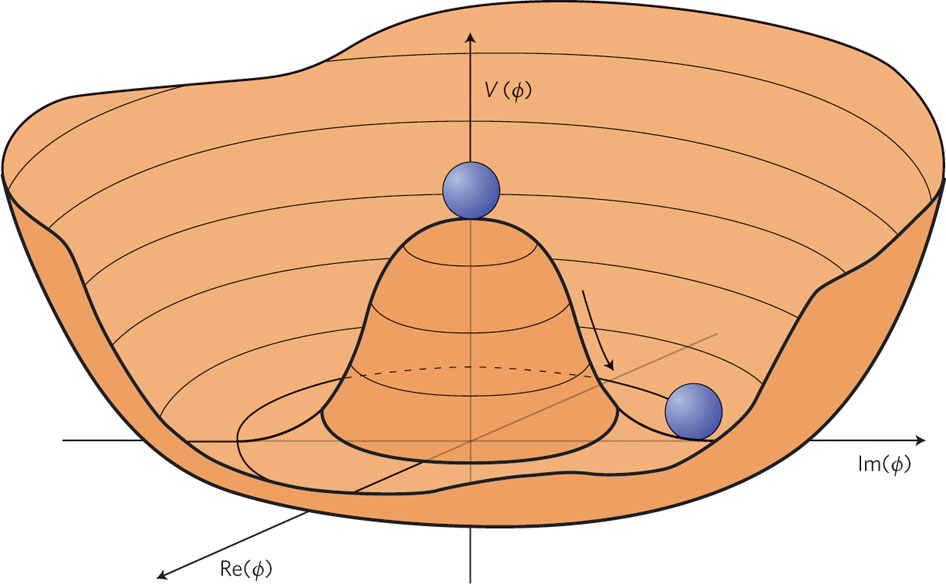
\includegraphics[scale=0.25]{THESISPLOTS/Higgs_Potential.jpg}
\captionof{figure}{Higgs boson "Mexican hat" potential, $V(\phi^{*}\phi) = \mu^{2}(\phi^{*}\phi) + \lambda(\phi^{*}\phi)^{2}$, which leads to spontaneous symmetry breaking with choice of parameters $\mu^{2} < 0$, $\lambda > 0$.}
\label{fig:Higgs}
\end{center}
\end{minipage}

\vspace{5mm}
\begin{minipage}{0.90\linewidth}
\begin{center}
\centering
%\mbox{
%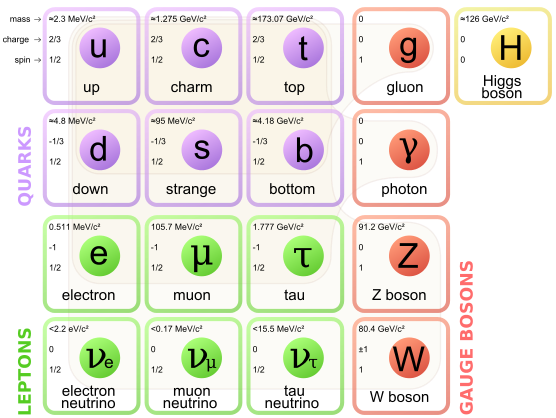
\includegraphics[scale=0.5]{THESISPLOTS/Standard_Model_of_Elementary_Particles.png} 
%\vspace{1cm} 
%\quad
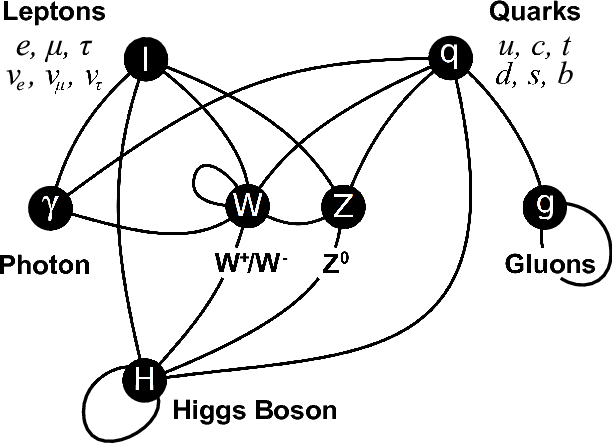
\includegraphics[height=0.5\textwidth, width=0.7\textwidth]{THESISPLOTS/SM_Particles.png}%}
\captionof{figure}{Fermions and bosons and their interactions in the SM. The bosons~(except the Higgs boson) mediate the interactions between fermions.}
\label{fig:ALLSM}
\end{center}
\end{minipage}
\vspace{5mm}

%%% SM Fermions and Bosons
\begin{minipage}{0.90\linewidth}
\begin{center}
%\bfseries{Supersymmetry multipletes and spin }
\begin{tabular}{c|*{3}{c}|c}
\toprule
\bfseries{Fermions} &

 \multicolumn{3}{|c|}{\bfseries {Generation}} 
 
  & \bfseries{Charge} \\
\hline \hline
 &  \texttt{First} & \texttt{Second} & \texttt{Third} &  \\
\hline
         &  &  &  &  \\
% & $ {\begin{pmatrix} \texttt{electron} \\ \texttt{electron neutrino}  \end{pmatrix} } $ &
%          $ {\begin{pmatrix} \texttt{muon} \\ \texttt{muon neutrino}  \end{pmatrix} } $ &
%          $ {\begin{pmatrix} \texttt{tau} \\ \texttt{tau neutrino}  \end{pmatrix} } $ &  \\    
Leptons & $ {\begin{pmatrix} \Pe^{-} \\ \Pnue  \end{pmatrix} } $  &  ${\begin{pmatrix} \Pmu^{-} \\ \Pnum \end{pmatrix} }$ &  ${\begin{pmatrix} \Ptau^{-} \\ \Pnut  \end{pmatrix} }$ &  ${\begin{pmatrix} -1 \\ 0  \end{pmatrix} }$ \\
         &   &   &  &  \\
\bottomrule  
          &  &  &  &  \\

% & $ {\begin{pmatrix} \texttt{up} \\ \texttt{down}  \end{pmatrix} } $ &
%          $ {\begin{pmatrix} \texttt{charm} \\ \texttt{strange}  \end{pmatrix} } $ &
%          $ {\begin{pmatrix} \texttt{top} \\ \texttt{bottom}  \end{pmatrix} } $ &  \\    
 Quarks  & $ {\begin{pmatrix} \Pup \\ \Pdown  \end{pmatrix} } $  &  ${\begin{pmatrix} \Pcharm \\ \Pstrange  \end{pmatrix} }$  &  ${\begin{pmatrix} \Ptop \\ \Pbottom  \end{pmatrix} }$ &  ${\begin{pmatrix} +\frac{2}{3} \\ -\frac{1}{3}  \end{pmatrix} }$ \\
         &  &  &  &  \\
\hline 
\bottomrule
\end{tabular}
\captionof{table}{Fermions of the SM. Particle symbols are explained in text.}
\label{tab:FermionsSM} 
\end{center}
\end{minipage}

\vspace{20mm}

\begin{minipage}{0.90\linewidth}
\begin{center}
%\bfseries{Supersymmetry multipletes and spin }
\begin{tabular}{c|c|c|c}
\toprule
\bfseries{Bosons} & \bfseries {Interaction} & \bfseries {Symmetry} & \bfseries{Characteristic Lifetime} \\ \hline
\PWpm,\PZ & Weak & $SU(2)_{L} \otimes U(1)_{Y}$ &  $10^{-8}$ to $10^{-13}$~seconds  \\
          &    &   &   \\
\Pphoton  & Electromagnetic & $ U(1)_{Q}$ & $10^{-14}$ to $10^{-20}$~seconds  \\
          &    &    &   \\
\Pgluon   & Strong   & $SU(3)_{C}$ &   $ < 10^{-22}$~seconds \\
          &    &     &   \\
\hline 
\bottomrule
\end{tabular}
\captionof{table}{Interaction mediating vector bosons in the SM and the characteristic lifetime of the interaction.}
\label{tab:BosonsSM} 
\end{center}
\end{minipage}

\clearpage

%%%%%%%%%%%%%%%%%%%%%%%%%%%%%%%%%%%%%%
\subsection{Beyond Standard Model Physics}
The Higgs boson is vital in the formulation and experimental success of the SM, yet the SM itself provides no explanation for the choice of parameters~($\mu^{2} < 0 $ and $ \lambda > 0$) of the  potential of the Higgs field which spontaneously breaks the gauge symmetry or whether only one type of Higgs field exists through which all fermions couple with to get their mass. Some  Beyond the Standard Model~(BSM) models, like \textit{Supersymmetry}, allow for the possibility of more than one Higgs field and predicts the existence of other particles in addition to those in the SM. The following are a few of the reasons for the interest we have developed in BSM physics, particularly Supersymmetry:

\subsubsection*{The Hierarchy Problem}
The prediction of the mass of the Higgs boson, $m^{2}_{H}$, by the SM include corrections, $\delta m^{2}_{f}$, arising from its coupling with fermions. These corrections, at one-loop level interactions of the Higgs boson with fermions like the one given by the Feynman diagram in Figure \ref{fig:HM}(a), can be computed in the SM as
\begin{equation}{\label{eq:HFermion}}
\delta m^{2}_{f} = \frac{1}{16\pi^{2}}|\lambda_{f}|^{2}\left(-2\Lambda^{2} + 6m^{2}_{f}\ln\left(\frac{\Lambda}{m_{f}}\right) + ...\right), 
\end{equation}
where $\lambda_{f}$ is the coupling strength parameter of the Higgs boson to fermions with the interaction Lagrangian density written as $\lambda_{f}H\bar{f}f$. The parameter, $\Lambda$, represents an arbitrary high energy scale~(of the order $10^{18}$\GeV) known as the \textit{cut-off} energy scale. 
Because $\Lambda = 10^{18}\GeV$ is very large, we would expect the correction to the Higgs boson's mass to equally be very large eventually causing the Higgs boson's mass, $m^{2}_{H}$, to be very large.
However, the Higgs boson's mass measured from experiment is only about $125$~\GeVcc. A dilemma thus arises, if one is to trust the SM prediction of the Higgs boson's mass then why are all these large corrections to the Higgs boson's mass not observed in experiments as they are equally predicted by the SM?  This dilemma or problem is known as the \textit{Hierarchy problem} and the SM does not provide an explanation for it.
%%%%%

\vspace{5mm}
\begin{minipage}{0.95\linewidth}
\begin{center}
%\begin{figure}[ht]
\begin{minipage}[b]{0.45\linewidth}
\centering
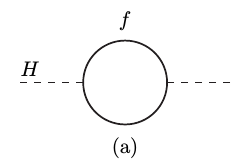
\includegraphics[height=0.5\textwidth,width=0.70\textwidth]{THESISPLOTS/Higgs_MassFermion.png}
%\captionof{figure}{Higgs fermion coupling}
%\label{fig:HMassL}
\end{minipage}
\hspace{0.5cm}
\begin{minipage}[b]{0.45\linewidth}
\centering
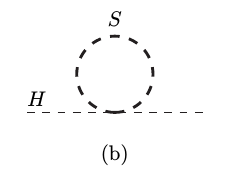
\includegraphics[height=0.5\textwidth,width=0.70\textwidth]{THESISPLOTS/Higgs_MassScalar.png}
%\caption{Higgs scalar coupling}
%\label{fig:HMassL}
\end{minipage}
%\end{figure}
\captionof{figure}{Higgs mass contributions arising from the Higgs field coupling to fermions~(a) and scalar~(b) fields.}
\label{fig:HM}
\end{center}
\end{minipage}

\vspace{5mm}
%\begin{center}
%\centering
%\mbox{
%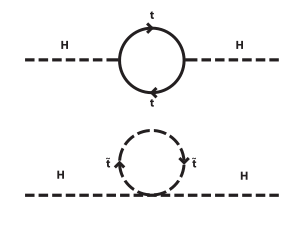
\includegraphics[height=5cm,width=0.5\linewidth]{THESISPLOTS/Higgs_Hirrachy_Problem.png}
%\captionof{figure}{Higgs self energy diagrams showing how the higgs boson mass is computed from both Higgs field and supersymmetric partner particle contributions.}
%\label{fig:Hmass}
%\end{center}
Supersymmetry~(SUSY), on the other hand, provides a plausible explanation as to why these corrections are not observed in experiments. In SUSY models, there are in addition to the scalar Higgs boson new supersymmetric scalar particles, yet to be observed, which can also couple to the Higgs field as given by the one-loop interaction level Feynman diagram in Figure \ref{fig:HM}(b). The contributions to the Higgs boson's mass from these new scalar supersymmetric particles, $\delta m^{2}_{S} $, computed at the same order of one-loop as for the fermions is given as 
\begin{equation}{\label{eq:HScalar}}
\delta m^{2}_{S} = \frac{1}{16\pi^{2}}|\lambda_{S}|^{2}\left(\Lambda^{2} - 2m^{2}_{S}\ln\left(\frac{\Lambda}{m_{S}}\right) + ...\right) ,
\end{equation}
where $\lambda_{S}$ is the coupling strength parameter of the Higgs field to the new scalar particle with the Lagrangian density given as: $\lambda_{S}HS\bar{S}$.
An interesting observation comparing Equations \ref{eq:HFermion} to Equation \ref{eq:HScalar} up to the $\Lambda^{2}$-terms is that their signs are opposite.
This means that these opposite signs corrections to the Higgs boson's mass can cancel each other so that their net contribution to the Higgs mass, $m^{2}_{H}$, is zero. This cancellation which happens at all orders of magnitude of these corrections is the reason why the mass of the Higgs boson from experiment is only about 125\GeVcc.

\subsubsection*{Dark Matter and Long-Lived Particles}
There is ample evidence~\cite{DM} that dark matter~(matter which does not interact with light) exists in the universe, and if this form of matter is made of particles, then, the lifetime of a dark matter particle must be comparable to the age of the universe. Furthermore, dark matter particles must be neutral since they do not interact with light. Such neutral stable particles are not described by the SM and so dark matter particles if they exists should probably interact with ordinary matter in addition to gravity through a new kind of interaction.
\newline
Neutral meta-stable~(particles that are stable for a long period of time and then decay) called \textit{Long-Lived Neutral Particles}~(LLNP) also not described by the SM can decay into dark matter particles through new interactions. These LLNPs are predicted by many BSM models and they have lifetimes longer than the characteristic lifetimes of particles and interactions described by the SM as given in Table \ref{tab:BosonsSM}. 
In addition to SUSY explaining the stability of the Higgs boson's mass, it also predicts the existence of LLNPs which decay into particles which are candidates for dark matter particles with lifetime beyond those in the SM  \cite{SUSYDM,LSPDM,DMS,KOlive}. Such predictions have motivated many studies in theory and experiment of SUSY as an interesting candidate among other BSM models. The idea of experimentally finding LLNPs described by either SUSY or any other BSM model is certainly a motivation for the study presented in this thesis.
\clearpage
%The understanding of SUSY began with the \textit{Haag-Lapuszanski-Sohnius} theorem \cite{MSUSY}, in 1975, when the idea of supersymmetry generators or
%%%%%%%%%%%%%%%%%%%%%%%%%%%%%%%%%%%%%%%%%%%%%%%%%%%%%%%%%%%%%%%%%%%%%%%%%%%%%%%%%%
%%%%%%%%%%%%%%%%%%%%%%%%%%%%%%%%%%%%%%%%%%%%%%%%%%%%%%%%%%%%%%%%%%%%%%%%%%%%%%%%%%
\section{Supersymmetry}
%%%%%%%%%%%%%%%%%%%%%%%%%%%%%%%%%%%%%
Suppersymmetry relates space-time symmetries~(rotation and translation) to gauge symmetries~($SU(3)_{C}\otimes SU(2)_{L}\otimes U(1)_{Y}$) \cite{MSUSY,SALAM}. The generators of Supersymmetry~(SUSY), $\mathrm{Q}$, can transform fermions into bosons and bosons into fermions as
\begin{eqnarray}{\label{eq:SUSY}}
\mathrm{Q}|\textbf{Fermion}\rangle =|\textbf{Boson}\rangle,    &
\mathrm{Q}|\textbf{Boson}\rangle  =|\textbf{Fermion} \rangle , 
\end{eqnarray}
and as a consequence of this transformation, fermions and their corresponding bosons have the same mass in SUSY.

\subsection{The Minimal Supersymmetric Standard Model}
The \textit{Minimal Supersymmetric Standard Model}~(MSSM) is an extension of the SM using only one SUSY generator, $\mathrm{Q}$, in its formulation. Since the MSSM includes supersymmetric particles or \textit{sparticles} as they are called which are partners of SM particles, the number of particles in the MSSM is obviously doubled, however, the gauge symmetries are the same as in the SM. The spin of a  sparticle and its SM counterpart differ by half-integer.
\newline
In the MSSM, two complex Higgs doublets are required: $ \mathbf{H_{d}} = (H^{0}_{1},H^{-}_{1})$ and $ \mathbf{H_{u}} = (H^{+}_{2},H^{0}_{2})$, to give mass to the \textsf{Down}-typed quarks~(and leptons) and to the  \textsf{Up}-typed quarks, respectively. The particles interact with a superpontential of the Higgs bosons through dimensionless  Yukawa couplings to acquire their mass through spontaneous SUSY breaking. Details of the nature of these interactions and spontaneous SUSY breaking can be found in \cite{MSSM,SUSYM,SUSYN}. 
\newline
Bosons~(fermions) in the SM have superpartners which are fermions~(bosons) in SUSY as given in Tables \ref{tab:SUSYSMPART} and \ref{tab:SUSYS} which present the particles in the MSSM. The names of sparticles are derived from their SM counterparts by adding an "\textit{s}" in front of the SM particle name. For example, a \textit{selectron} is the supersymmetric partner of the electron, \textit{squarks} are the supersymmetric partners of SM quarks. Superpartners of the SM vector bosons are indicated with the suffix "-ino ", as in \textit{wino} and \textit{gluinos}. While the superpartners of SM fermions are scalars called \textit{sfermions}~($\tilde{l}$), like sneutrinos~($\tilde{\nu}$) and squarks~($\tilde{q}$), fermions like \textit{gluinos}~($\tilde{g}$) are the superpartners of the massless  gluons, the gauge bosons of the strong interaction and \textit{Winos} and \textit{Binos} are the  fermionic superpartners  of the SM vector bosons~(\PWpm,$ W^{0}$,$B$). 
\newline
The symbols of sparticles carry the " $\tilde{}$ " sign above the SM symbol to distinguish them from their SM counterparts. For example, if \Pquark is the symbol for a SM particle then its supersymmetric partner has the symbol: \Psquark. 

\vspace{10mm}
\begin{minipage}{0.90\linewidth}
\begin{center}
\centering
\begin{tabular}{*{3}{c}|*{3}{l}}
%\mbox{Supersymmetry multipletes and spin }
\toprule
\multicolumn{3}{c}{\bfseries{Standard Model}} & \multicolumn{3}{c}{\bfseries{Supersymmetry}} \\
\hline 
Particle & Symbol & Spin &  Particle & Symbol & Spin \\
\hline
quark  & \Pquark  & $\frac{1}{2}$ & squark & \Psquark &  $0$ \\
lepton &  \Plepton & $\frac{1}{2}$ & slepton & \Pslepton &  $0$ \\
\hline
 W bosons  & \PWpm,$ W^{0}$  & $1$ & Wino &  $\tilde{W}^{\pm}, \tilde{W}^{0}$ &  $\frac{1}{2}$ \\
B boson  & $B$   &  $1$ & Bino & \PSBino  &  $\frac{1}{2}$ \\
 gluon  & \Pgluon  &  $1$ & gluino & \PSgluino &  $\frac{1}{2}$ \\
Higgs bosons &   \PHiggsheavy($\times 4$)  & $0$ & higgsino & \PSHiggs($\times 4$)  & $\frac{1}{2}$ \\ 
\hline
Graviton & G & 2 & gravitino & $\tilde{G}$ & $\frac{3}{2}$ \\
\bottomrule
\end{tabular}
\captionof{table}{Particles in the MSSM. SUSY particles~(sparticles) have a " $\tilde{•}$ " on the symbol}
\label{tab:SUSYSMPART} 
\end{center}
\end{minipage}

\vspace{10mm}

\begin{minipage}{0.90\linewidth}
\begin{center}
\centering
\begin{tabular}{l|l| l}
%\mbox{Supersymmetry multipletes and spin }
\toprule
\bfseries{Particle Names} & \bfseries {Gauge eigenstates} & \bfseries{Mass eigenstates} \\ 
\hline \hline
squark & \Psquark  & \Psquark \\
\hline
slepton & \PSlepton & \PSlepton \\
\hline
Neutralinos & $\tilde{W}^{0},\tilde{B}^{0},\tilde{H}^{0}_{1},\tilde{H}^{0}_{2}$ &$\tilde{\chi}^{0}_{1},\tilde{\chi}^{0}_{2},\tilde{\chi}^{0}_{3},\tilde{\chi}^{0}_{4}$ \\
\hline
Charginos & $\tilde{W}^{+}, \tilde{W}^{-}, \tilde{H}^{+}, \tilde{H}^{-}$ & $\tilde{\chi}^{\pm}_{1}$,$\tilde{\chi}^{\pm}_{2}$ \\
\hline 
Higgs bosons & $H^{0}_{1}, H^{0}_{2}, H^{-}_{1}, H^{+}_{2}$ & $h^{0},H^{0},A^{0},H^{\pm}$ \\
\hline
gluino & $\tilde{g}$& $\tilde{g}$ \\
\hline
Gravitino & $\tilde{G}$& $\tilde{G}$ \\
\bottomrule
\end{tabular}
\captionof{table}{Gauge and mass eigenstates of SUSY particles in the Minimal Supersymmetric SM~(MSSM).}
\label{tab:SUSYS} 
\end{center}
\end{minipage}


\vspace{10mm}

\clearpage

The superpartners of these Higgs bosons~($H^{0}_{1}, H^{0}_{2}, H^{-}_{1}, H^{+}_{2}$) are fermions called \textit{higgsinos}~($\tilde{H}^{0}_{1}, \tilde{H}^{-}_{1}, \tilde{H}^{0}_{2},\tilde{H}^{+}_{2}$) while the superpartners of the gauge bosons are called \textit{gauginos}~($\tilde{B}^{0},\tilde{W}^{0},\tilde{W}^{-},\tilde{W}^{+}$). 
The neutral gauginos and higgsinos~($\tilde{B}^{0},\tilde{W}^{0},\tilde{H}^{0}_{1},\tilde{H}^{0}_{2}$) mix quantum mechanically to form four neutral fermions called \textit{Neutralinos}~($\tilde{\chi}^{0}_{1},\tilde{\chi}^{0}_{2},\tilde{\chi}^{0}_{3},\tilde{\chi}^{0}_{4}$), and the charged gauginos and higgsinos~($\tilde{W}^{-},\tilde{W}^{+},\tilde{H}^{-}_{1},\tilde{H}^{+}_{2}$) mix quantum mechanically together to form four charged fermions called \textit{Charginos}~($\tilde{\chi}^{\pm}_{1}$,$\tilde{\chi}^{\pm}_{2}$). The masses of the neutralinos and charginos depend on the mixing parameters which include the masses of the gauginos and higgsinos and are model dependent.

%%%The gauge and mass eigenstates of fermionic supersymmetric particles in the MSSM are also shown.
%\clearpage
%\subsubsection{Supersymmetry Breaking}

%\subsubsection{Double Higgs}

% whose Lagrangian density can be written as 
%\begin{align}{\label{eq:SUSYEQ}}
%W_{\mbox{MSSM}} = \bar{u}\mathbf{y_{u}}QH_{u}   -   \bar{d}\mathbf{y_{d}}QH_{d}   -  \bar{e}\mathbf{y_{e}}LH_{d}  -  \mu H_{d}H_{u}
%\end{align}
%. $H_{u}$, $H_{d}$, $ Q$, $L$, $\bar{u}$, $\bar{d}$, $\bar{e}$ are chiral superfields of the chiral supermultiplets~(spin-1/2 and spin-0 files),.
%The 
%These can mix to form a pair of mass eigenstates called \textit{charginos}~($\tilde{\chi}^{\pm}_{j}, j=1,2$), \ie,
%$\tilde{\chi}^{\pm}_{1,2}$ are mixtures of $\tilde{W}^{+}, \tilde{W}^{-}, \tilde{H}^{+}, \tilde{H}^{-} $ and a quartet of mass  eigenstates called \textit{neutralinos}~($\tilde{\chi}^{0}_{i}, i=1,...,4$), \ie, $\tilde{\chi}^{0}_{1-4}$ are mixtures of $\tilde{B}^{0}, \tilde{W}^{0}, \tilde{h}^{0}, \tilde{H}^{0} $.
%\newline

%\paragraph*{R-Parity Symmetry}\mbox{}\\
\subsubsection{R-Parity}
It is acceptable in principle in SUSY to include terms in the MSSM Lagrangian density which may not conserve quantum numbers like the \textit{baryon}~($B$) and \textit{lepton}~($L$) numbers. However, in practice a consequence of adding such terms, for example, is that these terms leads to predictions of the proton's lifetime which is much shorter than what is measured in experiments. Since there are no evidence of such phenomenons like the proton decay which violate these quantum numbers, SUSY models are constructed with the introduction of an additional matter symmetry called \textit{R-Parity} which relates quarks to leptons through their baryon and lepton numbers. R-parity is defined as
\begin{equation}
R_{P} = \left(-1\right)^{3(B-L) + 2S}
\end{equation}
where $S$ is the particle's spin.
%R-parity is a conserved quantum number which originates from a discrete $Z_{2}$-symmetry \cite{SM}. R-parity symmetry commutes with supersymmetry.
% Therefore, particles in a given supermultiplet do not have the same R parity.
SM particles like quarks have an \textit{even} R-parity, $R_{P} = 1$, while sparticles like squarks have \textit{odd} parity $R_{P} = -1$.
\newline
The phenomenological consequence of R-parity conservation are the following: first, in the decay of sparticles, the lightest sparticle~(LSP) have odd parity, $R_{P} =-1$, it is electrically neutral and considered to be absolutely stable. This makes the LSP a good dark matter candidate particle \cite{SUSYDM,KOlive}; second, every sparticle produced will eventually decay into an odd number of LSPs, third, sparticles can only be produced in pairs.
These phenomenological consequences of R-parity makes \textit{R-parity Conserving}~(RPC) SUSY models very attractive for experimental studies since these models predict new particles with low enough masses which may be produced at current particle colliders like the LHC with unique experimental signatures like small missing transverse energy.

%%%%%%%%%%%%%%%%%%%%%%%%%%%%%%%%%%%%%%%
%%%%%%%%%%%%%%%%%%%%%%%%%%%%%%%%%%%%%%%%
\subsubsection{Cross Sections, Decay Rate and Branching Ratio}\label{LHCSUSY}
%%%%%%%%%%%%%%%%%%%%%%%%%%%%%%%%%%%%%%%%%%%%%%%%%%%%%%%%%%%%
\paragraph*{Cross Section} \mbox{}\\
Cross section provides a way of counting the number of particles produced at a proton-proton~($pp$) collider like the LHC. It is proportional to the probability  that the proton beams will collide and interact in a certain way to produce the particle. The cross section of producing a new particle in a BSM model or supersymmetric particle~(sparticle) at the LHC depends on the following: the available energy of the proton beams compared to the mass of the particle, the type of interaction or size of the couplings during collision and the flux of the proton beams, which affects the luminosity.
Since the predicted masses of sparticles are higher than those of their SM counterparts, we expect very few sparticles, if any, to be produced at the LHC, and even less for higher mass sparticles.
The typical cross section of producing a sparticle at the LHC is of the order of $1~pb =10^{-12}\times 10^{-24}~\cm^{2}$ or much smaller, $1~fb = 10^{-15}\times 10^{-24}~\cm^{2}$ for extremely rare SUSY or BSM  processes. This is very small compared to standard model processes like the production of the $\PZ$ or $\PWpm$ bosons which are of the order of a few $nb = 10^{-9}\times 10^{-24}~\cm^{2}$.
\newline
Sparticles are most likely to be produced at the LHC through the process of strong interactions~($pp \rightarrow \PSgluino\PSgluino, \PSq\PSq$) than through electro-weak interactions~($pp \rightarrow \PScharginopm\PScharginomp, \PSneutralino\PScharginopm$). This is because the cross section for strong interaction processes is larger than for electro-weak interactions. Figure \ref{fig:SUSYPROD}, shows the cross section of producing a sparticle, on the vertical y-axis, against its mass, on the horizontal x-axis, and the number of events produced, on the z-axis.
Looking at this plot, with 20\fbinv of LHC integrated luminosity~(luminosity relates the cross section to the numbers of events produced) of data from $pp$ collisions at $\sqrt{s} = 8$\TeV, we expect to see many events for a given sparticle mass to be produced  at the LHC through strong interactions than through electro-weak interactions.

\vspace{5mm}
\begin{minipage}{0.95\linewidth} 
\begin{center}
\mbox{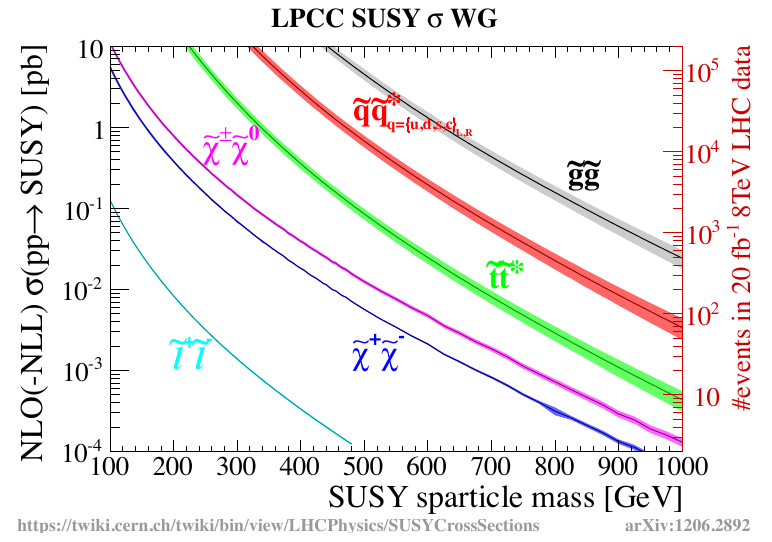
\includegraphics[height=0.67\textwidth, width=0.8\textwidth]{THESISPLOTS/SUSY_Xsec.png}}
%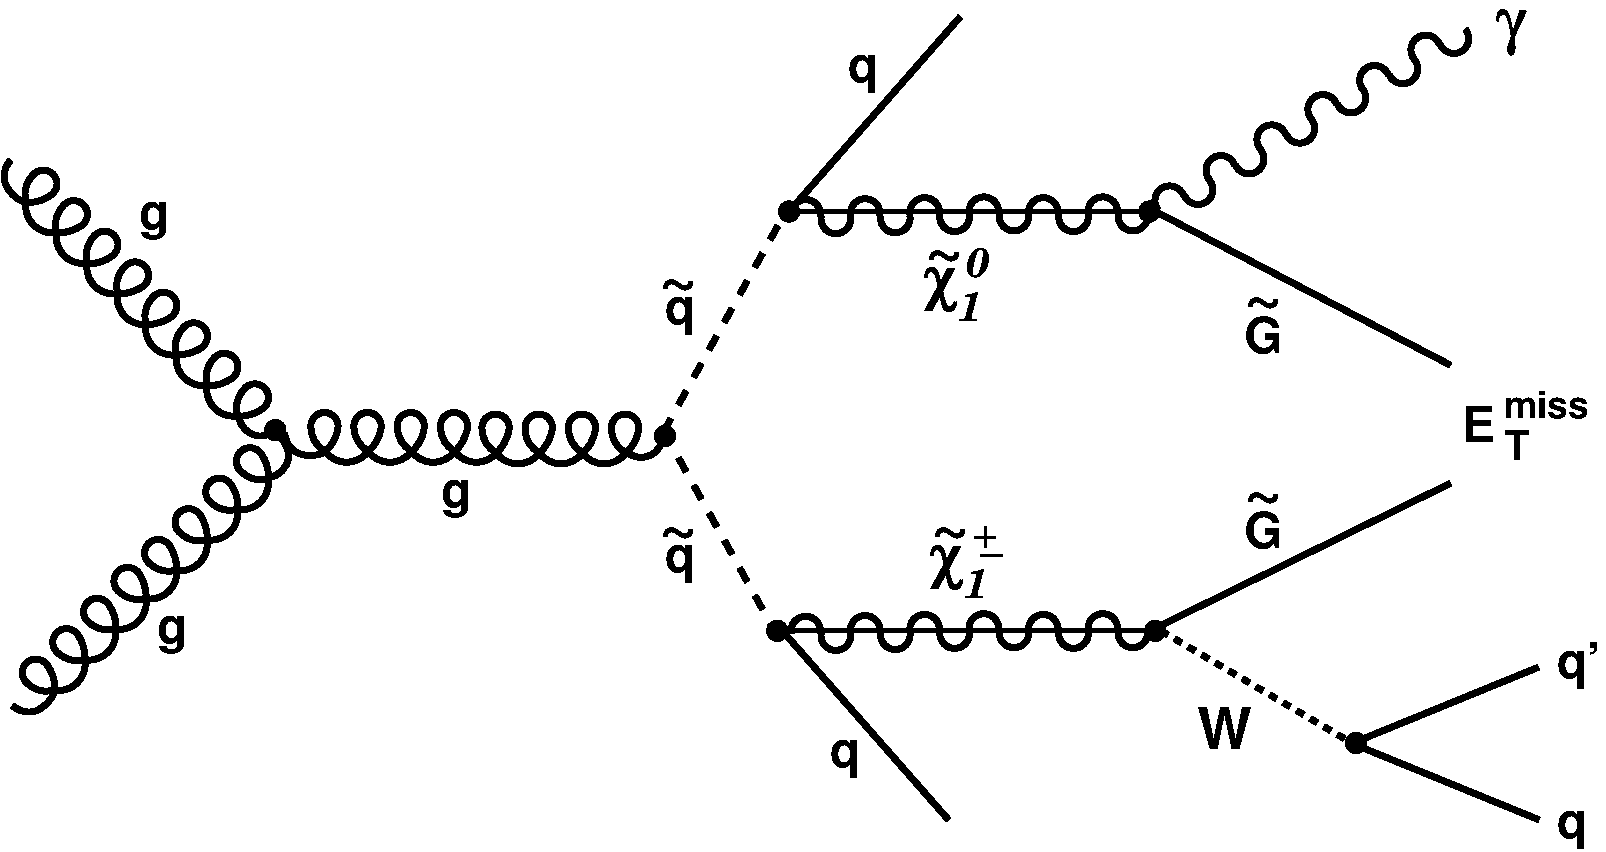
\includegraphics[width=2.5in]{THESISPLOTS/SinglePhoton_squark.pdf}} \\
\captionof{figure}{Cross section for producing sparticles with different mass and in different type of interaction at the LHC. More higher mass sparticles are produced through strong interaction, $pp \rightarrow \PSgluino\PSgluino$, than the others, $pp \rightarrow \PScharginopm\PScharginomp, \PSneutralino\PScharginopm$}
\label{fig:SUSYPROD}
\end{center}
\end{minipage}

%%\vspace{5mm}

%%%%%%%% DECAY %%%% LONG-LIVED%%%%%%%
\paragraph*{Decay Rate, Lifetime and Branching Ratio}  \mbox{}\\
The new particle or sparticle produced may decay either immediately or live for a while before it decays. The time it takes for the particle to stay stable after it was produced until when it finally decays is called its \textit{lifetime}. The particle's mean lifetime~($\tau$) is related to the decay rate also known as the \textit{decay width}~(\textbf{$\Gamma$}) as
\begin{equation}{\label{eq:RATE}}
  \tau = \frac{\hbar}{\Gamma}.
\end{equation}
The decay width is proportional to the probability that the particle will decay and this probability in general depends on the coupling strength or the mass difference between the particle and its decay products or daughter particles. The type of daughter particles produced from the decay depends on the likelihood that the parent particle would decay to those daughter particles or decay through that decay channel and this likelihood is defined as the ratio of the decay rate through that channel to the total decay rate of the parent particle through all possible decay channels. This channel "decay ratio" is known as the \textit{Branching Ratio}~(BR) for the given decay channel.
\newline
Particles with small mass differences or small couplings to their daughter particles have small decay widths and therefore live long  or have long lifetimes while those with large mass differences or large couplings have large decay widths or short lifetimes. A particle may decay through SM interactions like the strong interaction in which its mean lifetime is about $10^{-17}$ to $10^{-25}$~seconds, electromagnetic interaction in which its mean lifetime can be between $10^{-20}$ seconds to about $10^{-14}$ seconds and weak interaction in which its mean lifetime varies from $10^{-13}$ seconds to $10^{-8}$ seconds.
\newline
The type of long-lived particles we study in this thesis are those which do not decay through any of the SM interactions and have typical mean lifetimes ranging from a few nanoseconds~($10^{-9}$s) to hundreds of nanoseconds.
%In R-parity conserving models, sparticles are produced in pairs and each decay through a cascade decay  process into the LSP and its SM partner. 

%%%%%%%%%%%%%%%%%%%%%%%%%%%%%%%%%%%%%
\section{Gauge Mediated Supersymmetry Breaking Models}
%%%%%%%%%%%%%%%%%%%%%%%%%%%%%%%%%%%%%%%%%%%%%%%%%%
A consequence of SUSY is that sparticles and their SM partners have the same mass. Because no sparticle have been observed with the same mass as its SM counterpart, it means SUSY is not an exact symmetry of nature and must be broken. In order to break SUSY, SUSY must first be promoted to a local symmetry since it includes gravity in its description and the local SUSY breaking should happen such that the mass of sparticles are higher than their SM partners. In any local symmetry which is realized in the broken phase, the gauge particle becomes massive by eating the Numbu-Goldstone particle, and we expect the same for spontaneously broken local SUSY. Most theoretical models favor spontaneous local SUSY breaking because it preserves renormalisability in the theory, which is a characteristic of the SM model. 
\newline
Spontaneous local SUSY breaking is typically realized by introducing  \textit{soft} SUSY-breaking terms into the Lagrangian density. These soft terms ensure that those coupling constants which might lead to quadratic divergence are not introduced and the mass of the sparticles are predicted to be at about the \TeV energy scale, which is accessible to present particle colliders \cite{SUSYM,SUSYN}.
\newline
Often, the local SUSY breaking happens in the so-called \textit{Hidden Sector} and can be mediated to the MSSM sector through interactions which do not change the flavor of the particles called \textit{flavor blind interactions}, \eg gauge interactions \cite{SUSYBOOK}. The energy scale of the hidden sector is represented by an \textit{order parameter}, $\mathbf{F}$, which is the Vacuum Expectation Value~(VEV) of an auxiliary field responsible for SUSY breaking through some kind of \textit{Super-Higgs mechanism}. The order parameter or fundamental SUSY breaking energy scale measures the magnitude of the SUSY breaking in the vacuum state. 
\newline
In this super-Higgs mechanism the spin $\frac{1}{2}$ Goldstino becomes the longitudinal component of the spin $\frac{3}{2}$ gravitino~($\tilde{G}$), the superpartner of the graviton which mediates gravitational interactions. The gravitino acquires a mass during the process which is given as
\begin{equation}{\label{eq:GRAVITINO}}
m_{\tilde{G}} =  \frac{\mathbf{F}}{\sqrt{3}\mathrm{M}_{Pl}} \simeq \left(\frac{\sqrt{\mathbf{F}}}{100\TeV}\right)^{2} \eV,
\end{equation}
where $\mathrm{M}_{Pl} = 2.4 \times 10^{18}$\GeVcc is the reduced Planck mass and  the order parameter,  $\mathbf{F}$, has units of $[\mbox{mass}]^{2}$.

SUSY models in which the SUSY breaking is mediated through gauge interactions by \textit{Messenger} particles from the hidden sector to the MSSM sector are called \textit{Gauge Mediated Supersymmetry Breaking}~(GMSB) models \cite{GMSB}. Depending on the GMSB model there are $\mathbf{N}_{\mbox{mess}}$ generations of messenger fields with a general SUSY mass  of $\mathbf{M}_{\mbox{mess}}$. The simplest GMSB models with minimal gauge mediation assumes the messenger fields to be in the irreducible representations of dimension $\mathbf{5} \oplus \bar{\mathbf{5}}$  of an $SU(5)$ gauge group. The  $SU(5)$ group incorporates the SM gauge groups,  $SU(5) \supseteq  SU(3)_{C} \otimes SU(2)_{L} \otimes U(1)_{Y}$. The messenger field supermultiplet has scalar and fermion components which during SUSY breaking are split by an order parameter, $F_{m}$. As a consequence of this splitting gauginos in the MSSM get their mass  given as 

\begin{equation}{\label{eq:GMass}}
M_{a} = k_{a}\mathbf{N}_{\mbox{mess}}\mathbf{\Lambda}\frac{\alpha_{a}}{4\pi},
\end{equation}
through one-loop coupling with the messenger fields. The subscript, $a=1,2,3$, for Bino, Wino, and gluino, respectively, with $k_{1} = \frac{5}{3}, k_{2} = 1 = k_{3}$ and $\alpha_{a}$ is  the coupling strength. The effective MSSM or visible sector SUSY breaking parameter, $\mathbf{\Lambda}$, relates the messenger field splitting order parameter to the messenger particle SUSY mass in the following way:
\begin{equation}{\label{eq:DefLAMBDA}}
\mathbf{\Lambda} = F_{m} / \mathbf{M}_{\mbox{mess}}.
\end{equation}
The mass of scalars in the MSSM arise from their two-loop coupling to the messenger fields and it is given as
\begin{equation}{\label{eq:GSMass}}
m^{2}_{\phi} = 2\mathbf{N}_{\mbox{mess}}\mathbf{\Lambda}\left[ \frac{5}{3}\left(\frac{Y}{2}\right)^{2}\left(\frac{\alpha_{1}}{4\pi}\right)^{2} + \textsf{C}_{2}\left(\frac{\alpha_{2}}{4\pi}\right)^{2} + \textsf{C}_{3}\left(\frac{\alpha_{3}}{4\pi}\right)^{2} \right],
\end{equation}
where $Y$ is the weak hyper charge normalized to $Q = T_{3} + \frac{Y}{2}$, same as in the SM, $\textsf{C}_{2} = \frac{3}{4}$ for weak isospin doublet scalars and zero for weak isospin singlets and $\textsf{C}_{3} = \frac{4}{3}$ for squarks and zero for other scalars.  
\par
It is possible that the fundamental SUSY breaking scale, $\mathbf{F}$, which determines the gravitino's mass given in Equation \ref{eq:GRAVITINO} is higher that the SUSY breaking scale, $F_{m}$, felt by the messenger fields. This difference is parameterized using a dimensionless parameter, $C_{grav}$, relating the parameters  $\mathbf{F}$ and  $F_{m}$ as 
\begin{equation}
C_{grav} = \mathbf{F} / F_{m}.
\end{equation}
If $C_{grav} = 1$ then only one energy scale determines and fixes the masses of all the sparticles in GMSB models and the Next-To-Lightest Supersymmetric Particle~(NLSP) decays instantaneously~(prompt) to the Lightest-Supersymmetric Particle~(LSP). If  $C_{grav} > 1$, the mass difference between the NLSP and the LSP is no longer fixed and the decay rate may vary from prompt to non-prompt. Therefore, $C_{grav}$ can be used to control the decay rate of the NLSP to the LSP and hence the lifetime of the NLSP from prompt to long-lived. The phenomenological consequences of GMSB models are interesting to study at experiments, for example, many GMSB models predict the existence of long-lived particles which can decay into gravitinos whose mass can be within the mass range of dark matter particles. The gravitino is a good candidate for dark matter since it is stable and neutral.
%%%%%%%%%%%%%%%%%%%%%%%%%%%%%%%%%%%%%%%%%%%%%%%%%%%%%%%%%%%%%%%%%%%%%%%%%%%%%%%%%%%%%%%%%%%%%%%%%%%%%%%%
\subsection{Long-Lived Neutral Particles in GMSB Models}\label{long-lived}
%%% Gravitino cooupling to other SUSY particles.
GMSB models describe gravitino interactions with other particles in the same supermultiplet such as \textit{gravitino-gaugino-gauge boson}~($\tilde{G},\lambda,\mathrm{A}$)(left) and \textit{gravitino-scalar-chiral fermion}~($\tilde{G},\phi,\psi$)~(right) interactions shown by the Feynman diagrams in Figure \ref{fig:feynman_grav}. These interactions allow for a sparticle~($\tilde{P}$) to decay into its SM partner~($P$) and the gravitino~($\tilde{G}$). Since the interaction coupling strength is proportional to $\frac{1}{\sqrt{\mathbf{F}}}$, the decay rate is suppressed.

\vspace{5mm}
\begin{minipage}{0.90\linewidth}
\begin{center}
\centering
\mbox{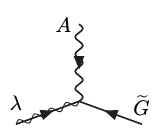
\includegraphics[height=0.3\textwidth, width=0.3\textwidth]{THESISPLOTS/Gravitino-Gaugino-Coupling.png} \quad
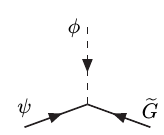
\includegraphics[height=0.3\textwidth, width=0.3\textwidth]{THESISPLOTS/Gravitino-Scalar-Coupling.png}
} 
\captionof{figure}{Feynman diagrams of\textit{Gravitino-Gaugino-Gauge boson}~($\tilde{G},\lambda,\mathrm{A}$)~(\textit{left}) and \textit{Gravitino-Scalar-Chiral fermion}~($\tilde{G},\phi,\psi$)~(\textit{right}) couplings. The coupling strength goes like $\frac{1}{\sqrt{\mathbf{F}}}$.}
\label{fig:feynman_grav}
\end{center}
\end{minipage}

\vspace{5mm}
The decay rate is given as
\begin{equation}{\label{eq:drate}}
\Gamma(\tilde{P} \rightarrow P + \tilde{G}) = \kappa \frac{ m^{5}_{\tilde{P}}}{16\pi\mathbf{F}^{2}}\left(1 - \frac{m^{2}_{P}}{m^{2}_{\tilde{P}}} \right)^{2}
\end{equation}
where $\kappa$ is a mixing parameter to be evaluated for different model parameters. If $P$ and  $\tilde{P}$ are unmixed states within the same supermultiplet, as in the decay of a slepton to a lepton and gravitino, $\kappa = 1$. For superpartner mass eigenstates which are a mixture of superpartners in different supermultiplets, $\kappa < 1$ is possible, \eg for Bino decay to photon and gravitino, $\kappa = \cos^{2}\theta_{W}$. The other terms in the decay rate are due to the nature of the interaction and also from the kinematic phase space integral where the mass of the gravitino can be neglected in the computation \cite{GMSB,NLSP}.
\newline
From Equation \ref{eq:drate}, we find that the decay width is larger for smaller values of the fundamental SUSY breaking parameter, $\mathbf{F}$, or equivalently for smaller masses of the gravitino since using Equation \ref{eq:GRAVITINO} and the relation between the fundamental SUSY breaking parameter and $C_{grav}$, $\mathbf{F} = C_{grav} \mathbf{\Lambda}\mathbf{M}_{\mbox{mess}}$, the gravitino's mass becomes,
\begin{equation}{\label{eq:GRAV}}
m_{\tilde{G}} = C_{grav}\cdot \frac{\mathbf{\Lambda}\mathbf{M}_{\mbox{mess}}}{\sqrt{3}\mathrm{M}_{pl}}.
\end{equation}
This confirms that $C_{grav}$ is the parameter to use for controlling the gravitino's mass and the lifetime of the NLSP and for a fixed mass of the NLSP determined by $\mathbf{\Lambda}$, the decay width of the NLSP can be varied  from small to large values. 
\newline
In a scenario where the sparticle, $\tilde{P}$, is not the Next-To-Lightest Supersymmetric Particle~(NLSP) the decay, $\tilde{P} \rightarrow P + \tilde{G}$, suffers from competition with other probably favorable decay channels and this decay process is not competitive enough to happen at a collider experiment. However, if  $\tilde{P}$ is the NLSP, then there is no competition and this decay always happens at a collider.
\par 
It is important to observe here that, if the mass of the NLSP, $m_{NLSP}$, is of the order of $100$\GeV or more and $\sqrt{\mathbf{F}} \ll 1000$\TeV, equivalent to saying $m_{\tilde{G}} \leq 1$\keV, then the above decay rate  is of the order that the  NLSP can be observed as a long-lived particle in detectors at the large hadron collider.
%%%%%%%%%%%%%%%%%%%%%%%%%%%%%%%%%%%%%%%%%%%%%%%%%%%%%%%%%%%%%%%%%%%%%%%%%%%%%%%%%%%%%%%%%%%%%%%%%%%%%%%
\subsubsection{Lightest Neutralino as a Long-Lived Neutral Particle}\label{NeutralinoDecay}
In the scenario where the NLSP is the lightest neutralino, \PSneutralinoOne, then its lifetime~($c\tau_{\PSneutralinoOne}$) for the decay into a photon and gravitino, $ \PSneutralinoOne \rightarrow \gamma + \tilde{G}$, derived from Equations \ref{eq:RATE} and \ref{eq:drate} is given as
\begin{equation}{\label{eq:ctau}}
c\tau_{\PSneutralinoOne} \approx \left(\frac{m_{\PSneutralinoOne,}}{\mbox{ GeV}}\right)^{-5}\left(\frac{\sqrt{\mathbf{F}}}{\mbox{TeV}}\right)^{4}[\mm],
\end{equation}
where we have neglected $\kappa$ as we focus on the most relevant parameters influencing the lifetime and in terms of $C_{grav}$ the lifetime becomes,
\begin{equation}{\label{eq:pdlength}}
c\tau_{\PSneutralinoOne} \approx C^{2}_{grav} \left(\frac{m_{\PSneutralinoOne}}{\mbox{GeV}}\right)^{-5}\left(\frac{\sqrt{\mathbf{\Lambda}\cdot\mathbf{M}_{\mbox{mess}}}}{\mbox{TeV}}\right)^{4}[\mm].
\end{equation}
The dependence of the lifetime on the effective SUSY breaking scale, $\mathbf{\Lambda}$, and $C_{grav}$ means for a fixed  mass of \PSneutralinoOne, $m_{\PSneutralinoOne}$, given by $\mathbf{\Lambda}$, we can scan the parameter space for different lifetimes of the lightest neutralino by varying $C_{grav}$, and for a fixed value of $C_{grav}$, we can also scan the parameter space for different masses of  \PSneutralinoOne by varying $\mathbf{\Lambda}$. Therefore, using $\mathbf{\Lambda}$ and $C_{grav}$ we can scan the entire parameter space for different masses and lifetimes of long-lived lightest neutralinos.
\par 
The full set of parameters which define a given GMSB model are the following:
\begin{equation}{\label{eq:mGMSB}}
\left\{ \mathbf{\Lambda}, \quad \mathbf{M}_{\mbox{mess}},\quad \mathbf{N}_{\mbox{mess}}, \quad \tan(\beta), \quad sgn(\mu),\quad C_{grav}\right\},
\end{equation}
with the meaning of each parameter given as follows:
\begin{itemize}
 \item $\tan(\beta) = \frac{v_{u}}{v_{d}}$, relates the VEVs: $v_{u}$ and $v_{d}$, of the two Higgs doublets in the MSSM which are themselves not known. In most models, $1.5 \le \tan(\beta) \le 60$.
 \item $sgn(\mu)$ defines the sign of the Higgs and Higgsino mass parameter, $\mu$, which is arbitrary in their potential. $sgn(\mu)$ appears in the neutralino and chargino mass mixing matrix.
\item $\mathbf{N}_{\mbox{mess}}$ is the number of messenger particles mediating SUSY breaking and also determines the masses of the MSSM sparticles with the mass of scalars proportional to $\sqrt{\mathbf{N}_{\mbox{mess}}}$, while the masses of gauginos is linear with $\mathbf{N}_{\mbox{mess}}$. For the lightest neutralino, \PSneutralinoOne, to be the NLSP, the value of $\mathbf{N}_{\mbox{mess}}$ must be small.  
\item $\mathbf{\Lambda}$ is the effective SUSY breaking energy scale at the visible sector with both the masses of the gauginos and scalars proportional to it. 
\item $\mathbf{M}_{\mbox{mess}}$ is the mass of the messenger particles and must be lower than $10^{16}\GeV$ to allow for low energy SUSY breaking to happen in order that the gravitino is the LSP. $\mathbf{M}_{\mbox{mess}}$ must also be, $\mathbf{M}_{\mbox{mess}} > \mathbf{\Lambda}$, in order to avoid charge and color breaking in the messenger particle sector. 
 \end{itemize}
Different choices for the values of these parameters will represent different scenarios for GMSB models.

%\subsection{Decay of supersymmetric particles in CMS detector}

\subsection{Benchmark Scenario}
In this thesis we study an R-parity conserving benchmark GMSB model called the \textit{Snowmass Point and Slopes}~(SPS8) \cite{SPS8}. In the SPS8 benchmark GMSB model, the GMSB parameters are chosen as
\begin{equation}
{\mathbf{M}}_{\mbox{mess}} = 2\mathbf{\Lambda}, \quad \tan(\beta)= 15, \quad \mathbf{N}_{\mbox{mess}} = 1,
\end{equation}
while $\mathbf{\Lambda}$ and $C_{grav}$ vary.
\newline
The LSP is the gravitino~($\tilde{G}$) and the NLSP is the lightest neutralino~(\PSneutralinoOne).
The \PSneutralinoOne is a mixture of the Bino~($\tilde{B}^{0}$), Wino~($\tilde{W}^{0}$) and higgsino~($\tilde{H}^{0}_{u},\tilde{H}^{0}_{d}$), and the decay to its SM partner and the gravitino  will depend on the choice of parameters which affect the mixing.  Since the parameters: $\Lambda$, $\tan\beta$, and $sgn(\mu)$ affect the mixing, these parameters have been chosen in the SPS8 benchmark GMSB model to maximize the branching ratio for the decay of the \PSneutralinoOne to a photon~($\gamma$) and a gravitino over the other possible SM partners: \PZ boson, $Z^{\prime}$ and a higgs boson~($H$) \cite{NLSP}.
\newline
We study the decay of the lightest neutralino, \PSneutralinoOne, as the Long-Lived Neutral Particle~(LLNP), to a photon and gravitino, $\PSneutralinoOne\rightarrow \Pphoton + \tilde{G}$, in order to understand the signal of an event with a late photon and missing transverse energy in the final state.
By varying $\mathbf{\Lambda}$ and $C_{grav}$, we study the production and decay of \PSneutralinoOne with different masses and lifetimes. 
\subsubsection{Supersymmetric Particle Mass Spectra}
The effective SUSY breaking energy scale parameter, $\mathbf{\Lambda}$, determines the masses of all sparticles in the MSSM and the mass of each sparticle increases with $\mathbf{\Lambda}$. The sparticle mass spectra are shown in Figure \ref{fig:spectra} for $\mathbf{\Lambda} = 100$\TeV~(left plot) and $\mathbf{\Lambda} = 180$\TeV~(right plot) for the same values of $C_{grav} = 93.5$ computed according to the SPS8 benchmark GMSB model. As shown in these Figures, the masses of the sparticles, including the mass of \PSneutralinoOne  is larger for $\mathbf{\Lambda} = 180$\TeV~($m_{\PSneutralinoOne} = 256$\GeVcc)~(right plot) than for $\mathbf{\Lambda} = 100$\TeV~($m_{\PSneutralinoOne} = 140$\GeVcc)~(left plot). This means that in order to expand our search towards heavier lightest neutralinos we must scan larger values of $\mathbf{\Lambda}$.

\vspace{5mm}
\begin{minipage}{0.90\linewidth}
\begin{center}
\centering
\mbox{
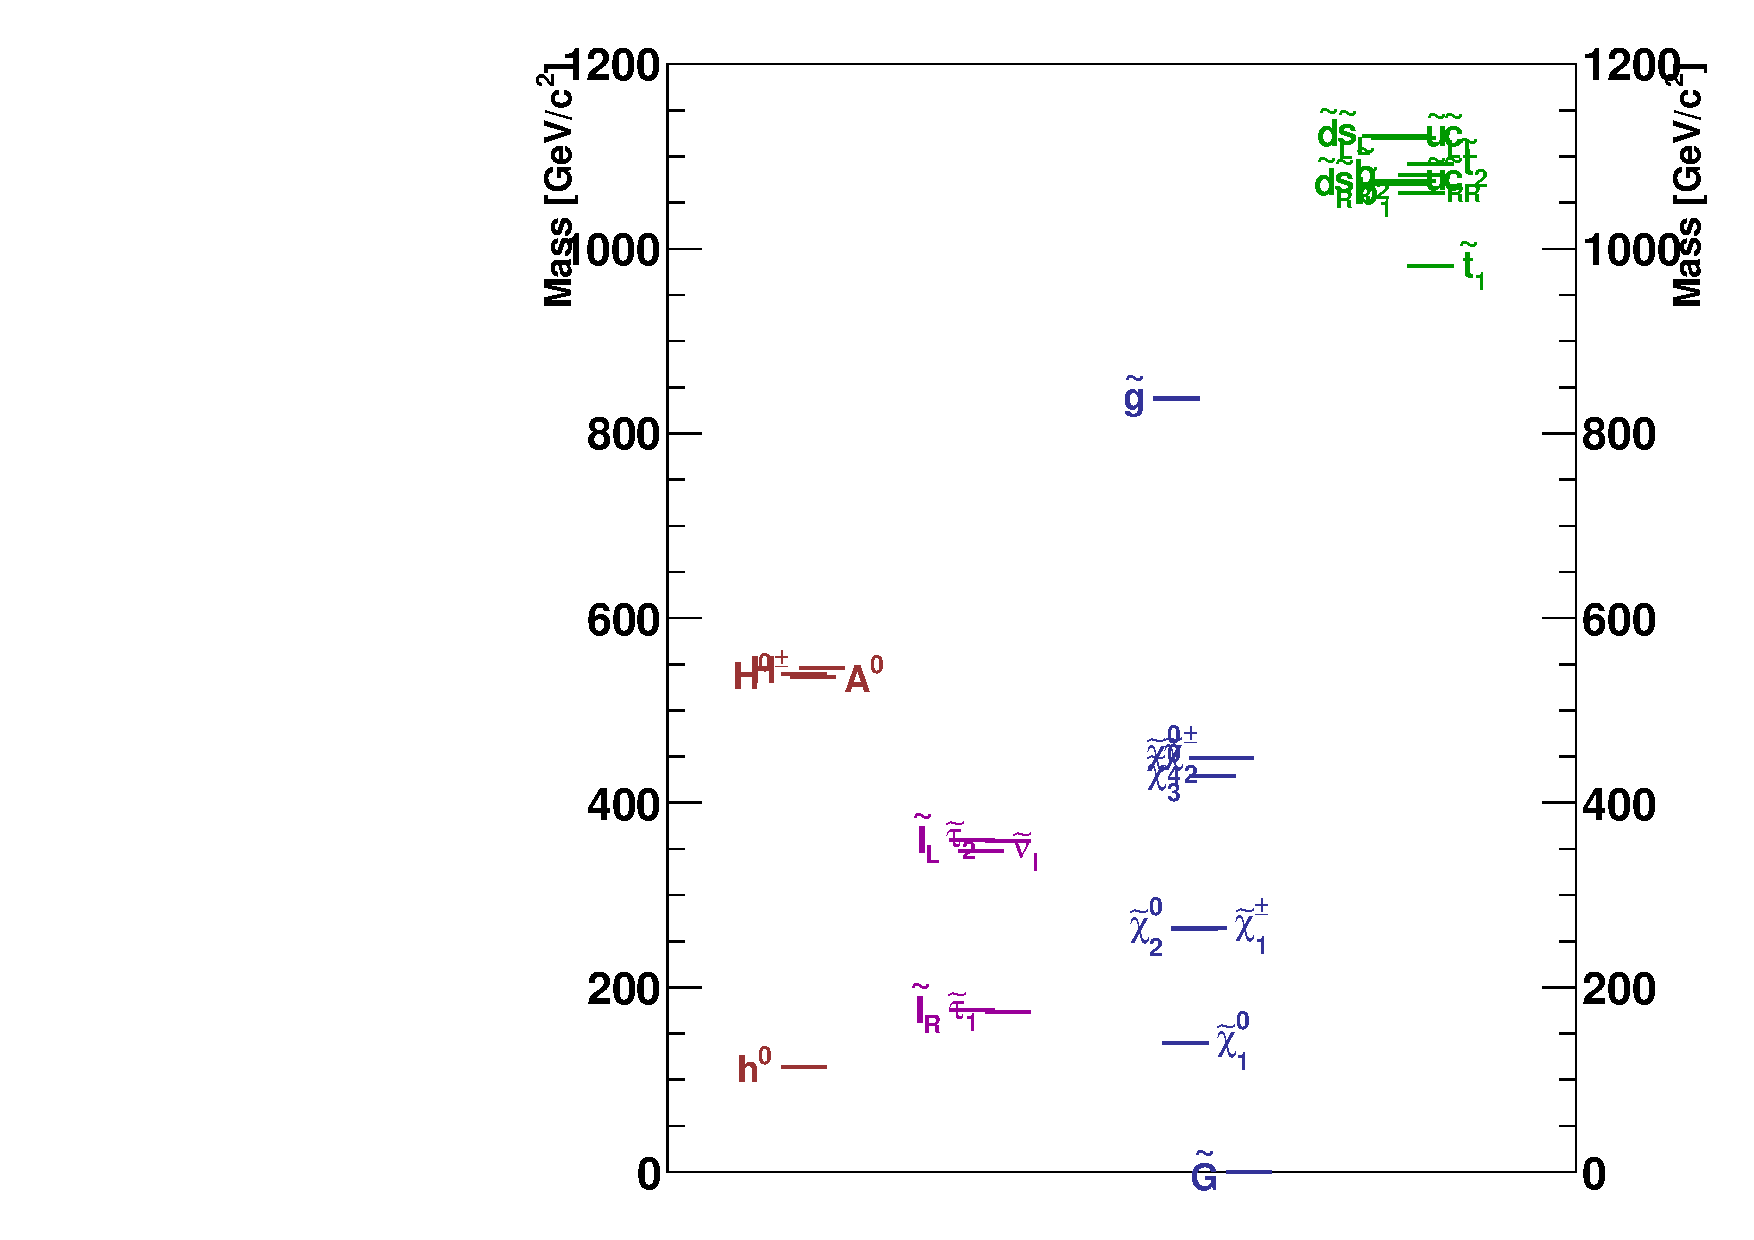
\includegraphics[height= 0.6\textwidth, width=0.5\textwidth]{THESISPLOTS/GMSB-Lambda100TeV-Spectrum.pdf} \quad
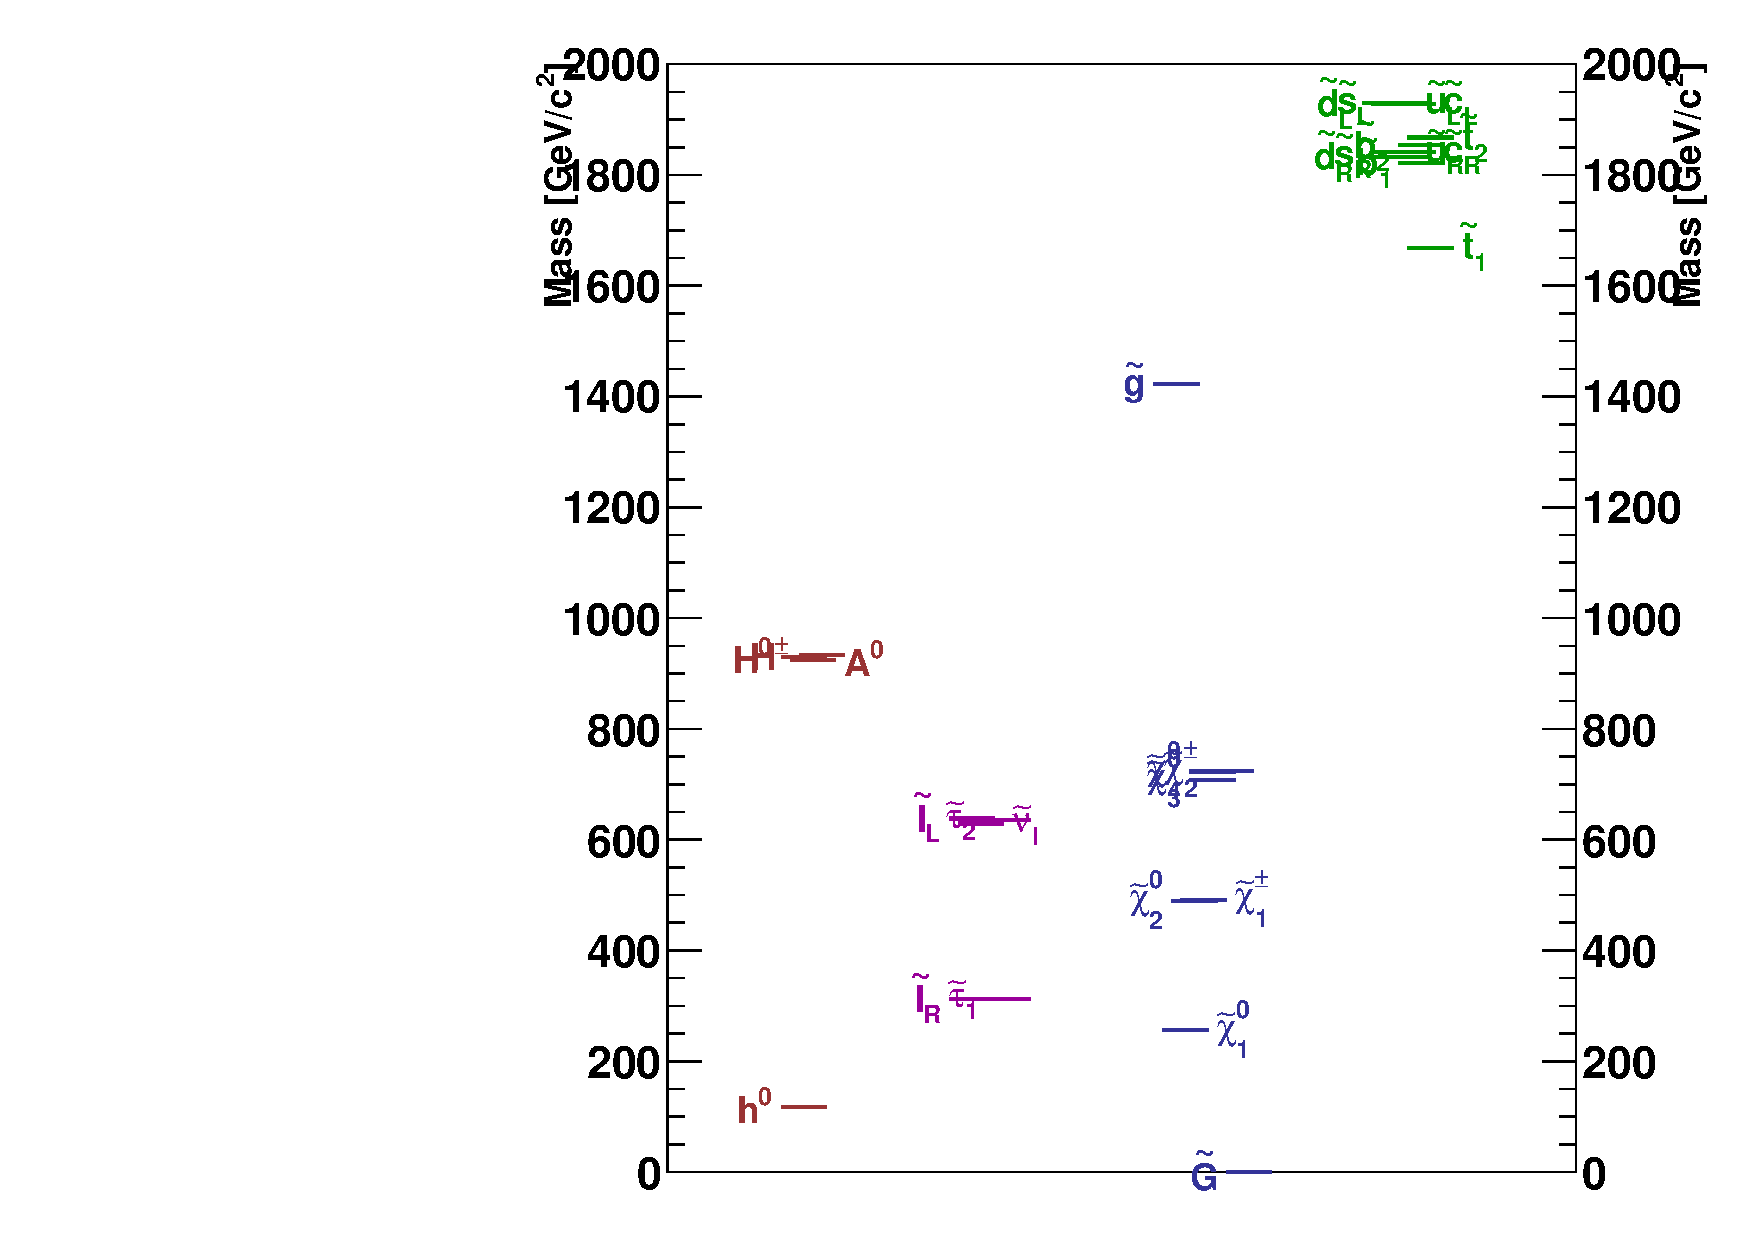
\includegraphics[height= 0.6\textwidth, width=0.5\textwidth]{THESISPLOTS/GMSB-Lambda180TeV-Spectrum.pdf}  
}
%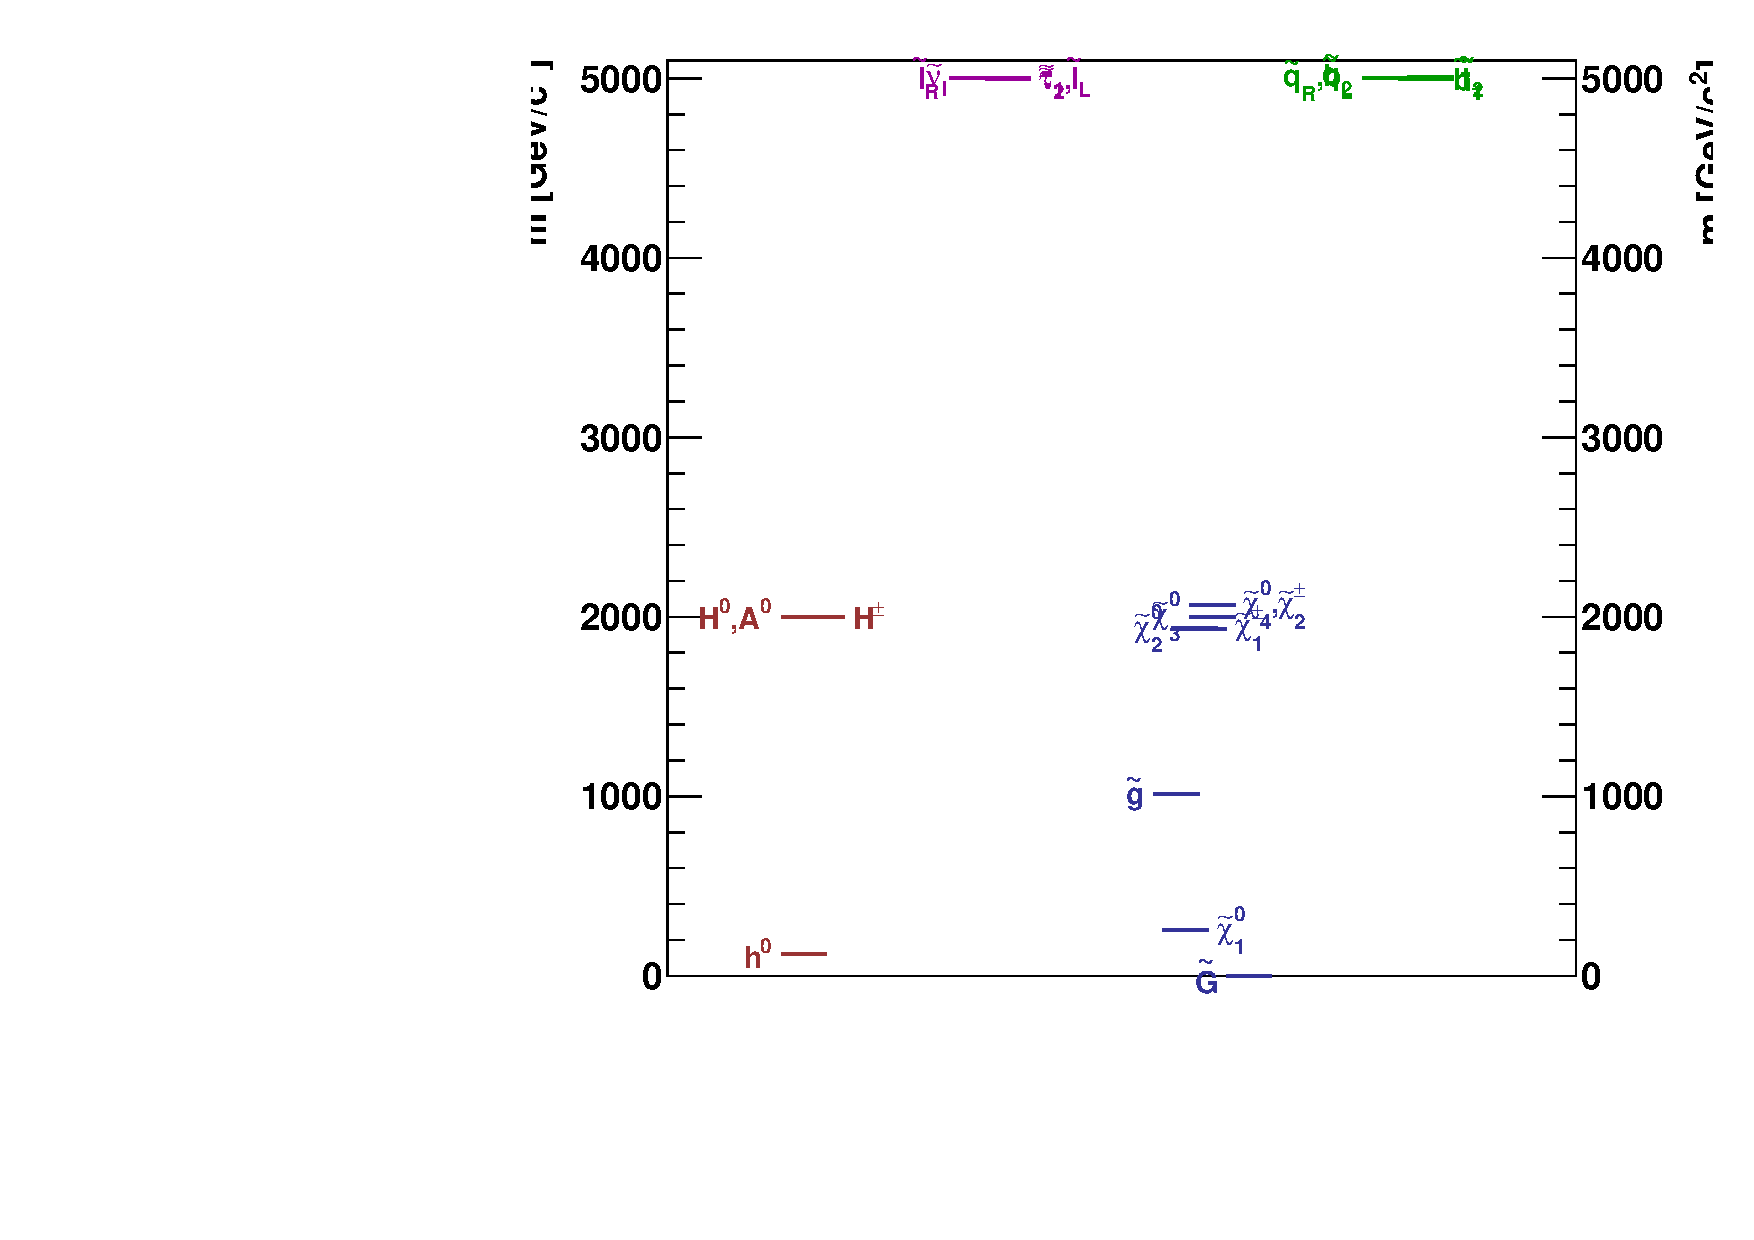
\includegraphics[height=2.5in]{THESISPLOTS/M3_1015_M1_255.pdf} }
\captionof{figure}{Sparticle mass spectra for SPS8 benchmark model: $\mathbf{\Lambda} = 100$\TeV~(left) and $\mathbf{\Lambda} = 180$\TeV~(right) with $C_{grav} = 93.5$. The sparticle mass increases with $\mathbf{\Lambda}$ }
%~(left) and GGM Model~(right) with mass of gluino ($M_{\tilde{g}} = 1.0$~ TeV)}
\label{fig:spectra}
\end{center}
\end{minipage}

%\vspace{5mm}

\subsection{Signal Modeling}
We are interested in the production of the lightest neutralino, \PSneutralinoOne, in strong interaction processes like $pp \rightarrow \PSgluino\PSgluino, \Psquark\Psquark$, since these processes have the highest production cross section at the LHC. The \PSneutralinoOne is produced indirectly as a decay product from the \textit{cascade decay} of massive sparticles like squarks~($\PSq$), excited squarks~($\PSq^{\star}$) and gluinos~($\PSgluino$). The Feynman diagrams in Figure \ref{fig:feynman_gsDiag} represent the different production and decay channels of \PSneutralinoOne through the cascade decay of gluinos and squarks.
The final state can either have two photons~(right Feynman diagrams) and two gravitinos if both \PSneutralinoOne  decay to a photon and a gravitino or a single photon~(left Feynman diagrams) if only one \PSneutralinoOne  decay to a photon and gravitino. The signal events must contain at least a single photon which is late relative to normal photons produced directly from nominal LHC $pp$ collisions and large Missing Transverse Energy~(\MET) in the final state. The \MET is due to the undetected gravitinos.

\vspace{5mm}
\begin{minipage}{0.88\linewidth}
\begin{center}
\centering
\mbox{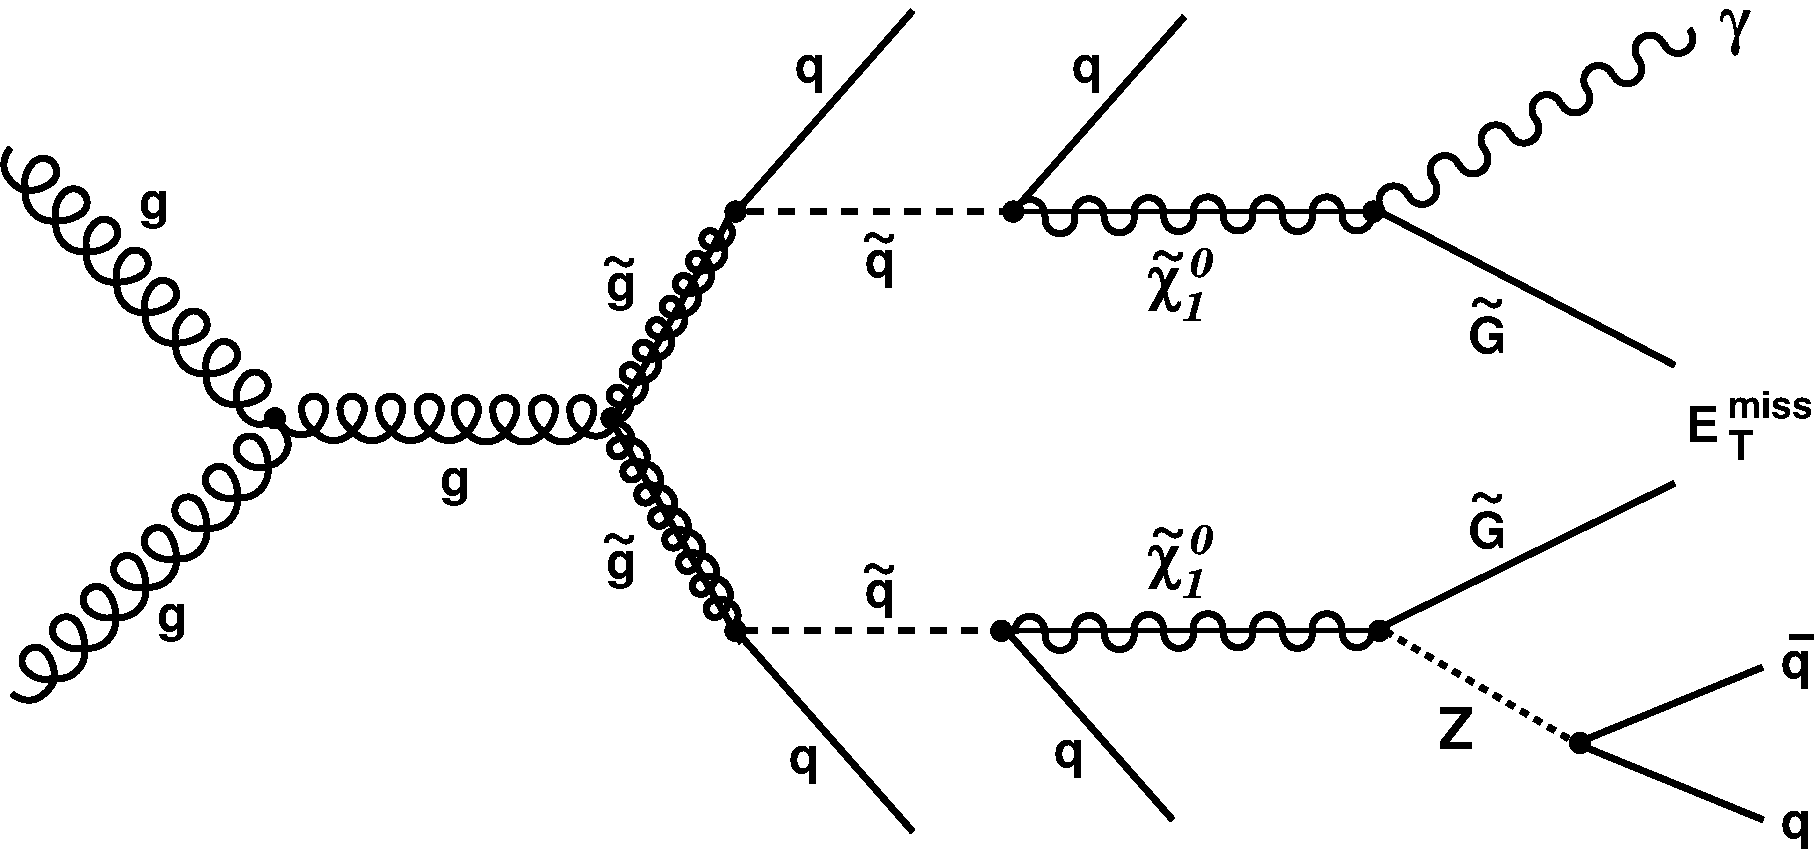
\includegraphics[height=0.7\textwidth, width=0.5\textwidth]{THESISPLOTS/SinglePhoton_gluino.pdf} \quad \quad
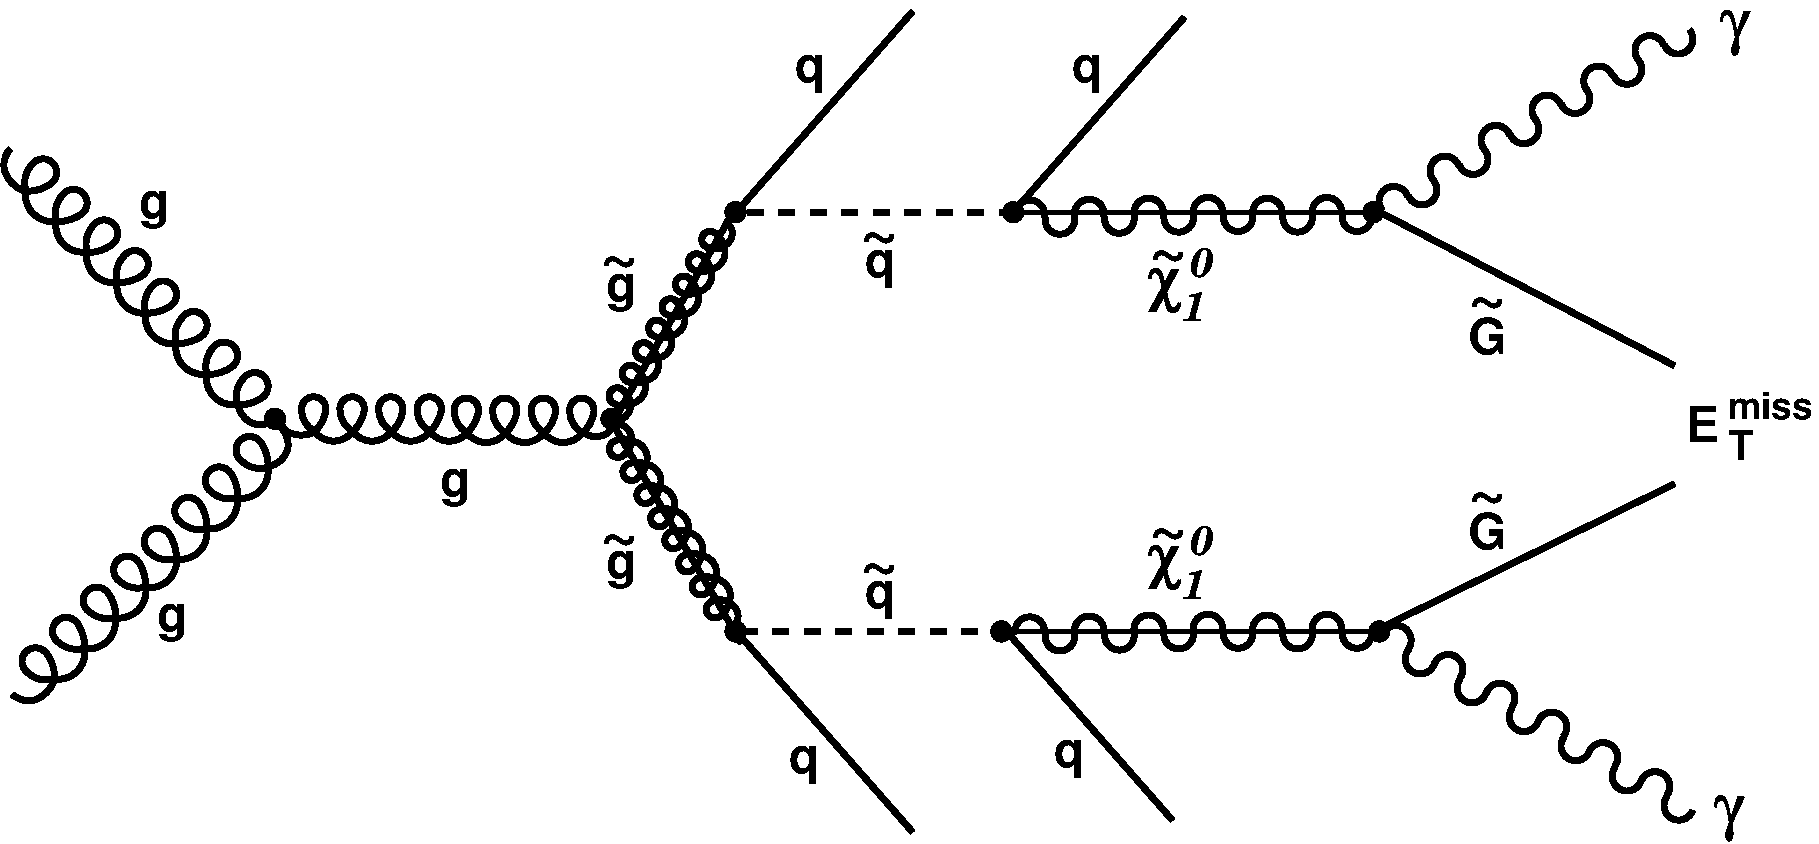
\includegraphics[height=0.7\textwidth, width=0.5\textwidth]{THESISPLOTS/Diphoton_gluino.pdf}} \\
\hspace{0.5cm}
\mbox{   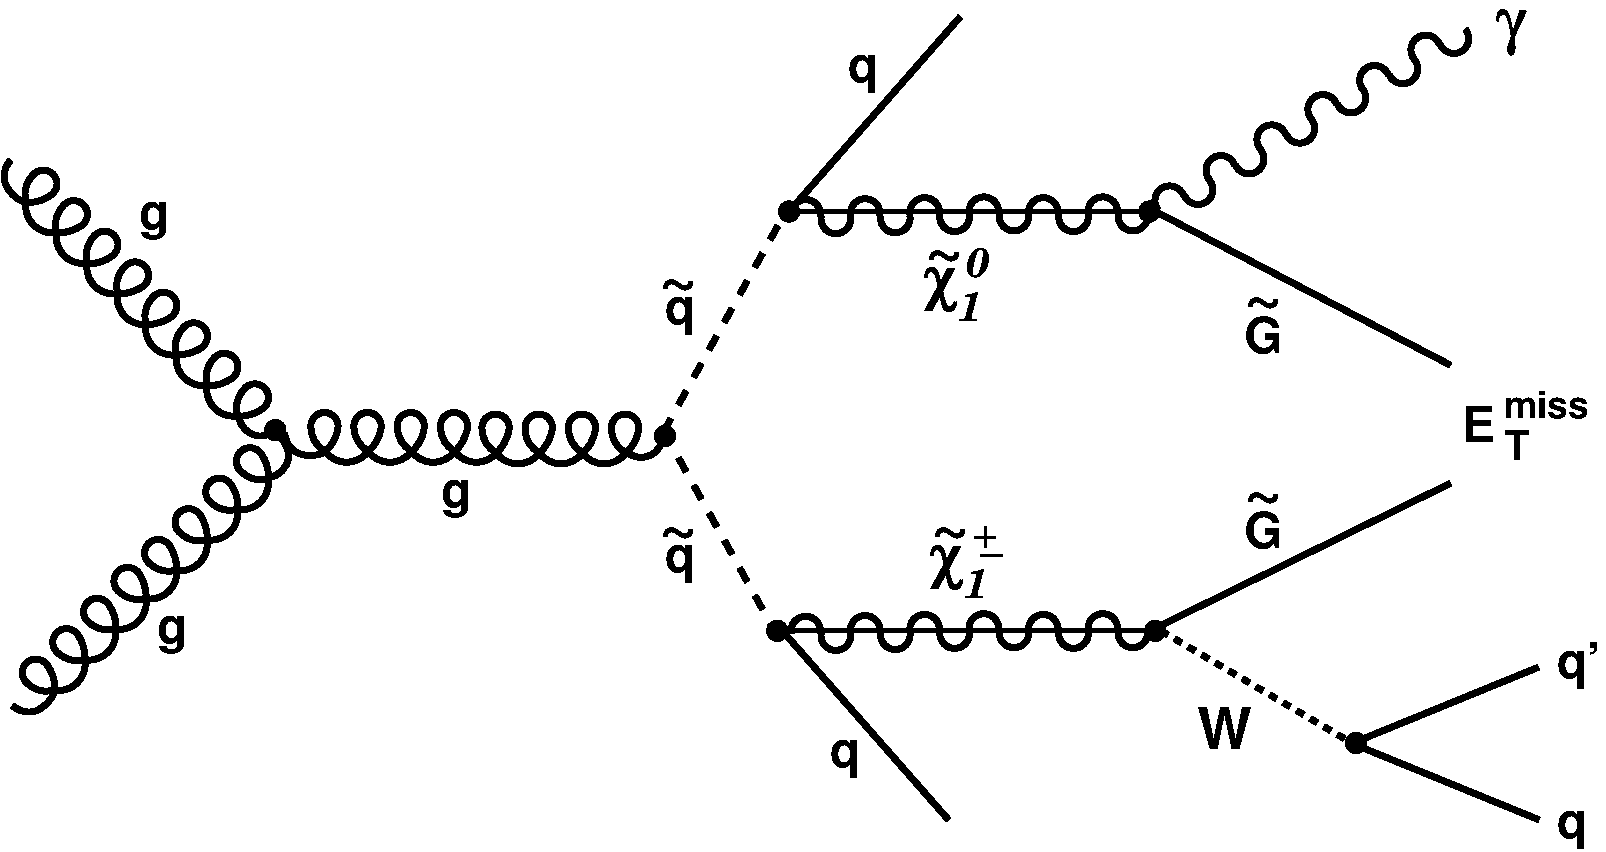
\includegraphics[height=0.7\textwidth, width=0.5\textwidth]{THESISPLOTS/SinglePhoton_squark.pdf}\quad \quad
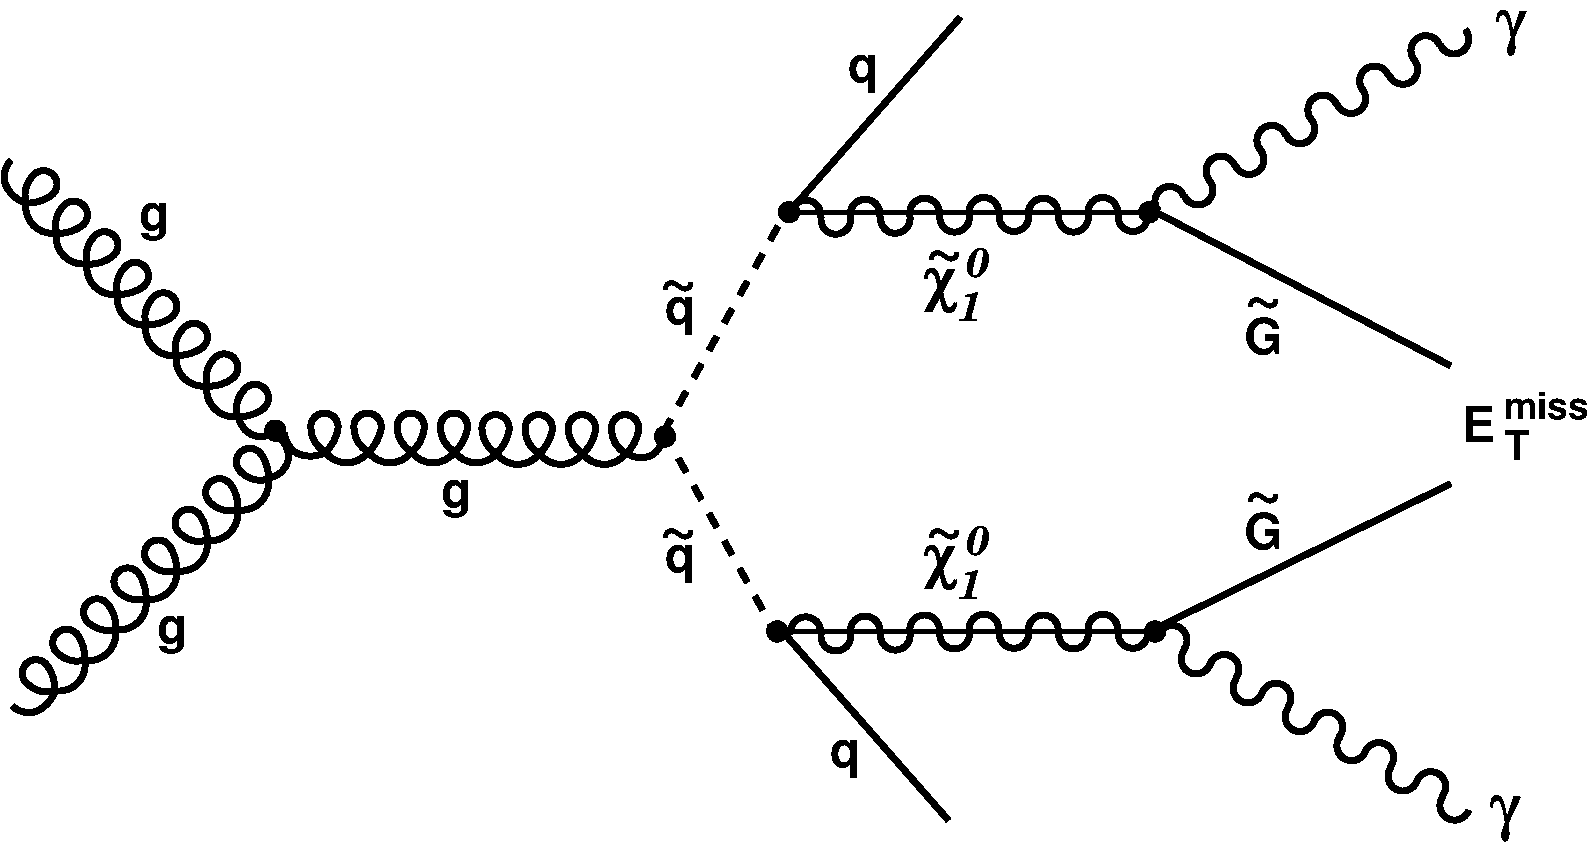
\includegraphics[height=0.7\textwidth, width=0.5\textwidth]{THESISPLOTS/Diphoton_squark.pdf} }
\captionof{figure}{Feynman diagrams for lightest neutralino~(\PSneutralinoOne) production from the cascade decay of a pair of gluinos~(\textit{top}) and squarks~(\textit{bottom}).
The final state can either have a single~(\textit{left diagrams}) or double photons~(\textit{right diagrams}).}
\label{fig:feynman_gsDiag}
\end{center}
\end{minipage}

%%\vspace{5mm}
\clearpage
%%%%%%%%%%%%%%%%%%%%%%%%%%%%%%%%%%%%%%%%%%%%%%%%%%%%%%%%%%%%%%%%%%%%%%%%%%%%%%%%%%%%%%%%%%%%%%%%%%%%%%% 
%produced according to the SPS8 benchmark GMSB model usin
We generate high-energy-physics signal events as might be produced during $pp$ collisions at the LHC with a center of mass energy, $\sqrt{s} = 8$\TeV, using a general-purpose event generator called \PYTHIA \cite{PYTHIA6}. The \PYTHIA software program is based on Monte Carlo~(MC) methods of numerical computations and takes as input a file containing the masses, interaction couplings, decay widths and all possible decay channels and Branching Ratio~($BR$) of every sparticle. This input file is called a \textit{SUSY Les Houches Accord}~(SLHA) file and it is the output of a sparticle production and decay simulation software program called \ISASUSY \cite{ISAJET}. In our case, the sparticle properties in each SLHA file have been produced according to the following choice of parameters of the SPS8 benchmark GMSB model:
%\begin{equation}\label{eq:SPS8PARM}
$sgn(\mu)= 1, \tan(\beta) = 15, \mathbf{N}_{\mbox{mess}} = 1, \mathbf{M}_{\mbox{mess}} = 2\mathbf{\Lambda}$,
%\end{equation}
with $C_{grav}$ and $\mathbf{\Lambda}$ chosen such that the signal event sample has events with a particular lightest neutralino mean lifetime~($c\tau$) and mass. The decay of the sparticles including the \PSneutralinoOne is simulated using \HDECAY, a software program which is part of \ISASUSY. We used \HDECAY to simulate the decay of the sparticles according to our SPS8 benchmark GMSB model.
\newline
The events were generated according to the processes described by the Feynmann diagrams in Figure \ref{fig:feynman_gsDiag} with the \PSneutralinoOne produced in the cascade decay of either a gluino or squark as: 
\begin{equation}
p+p \rightarrow \PSgluino\PSgluino, \PSq\PSq \rightarrow [\mbox{1 or 2 cascade decays}] \rightarrow 2\PSneutralinoOne + \mbox{jets} \rightarrow 2\Pphoton + 2\tilde{G} + \mbox{jets}.
\end{equation} 
The \PSneutralinoOne decays to either $\gamma$, $Z$, $H$, \EE, and the $\tilde{G}$. The dominant mode of decay is $\PSneutralinoOne\rightarrow \gamma + \tilde{G}$ with a decay branching fraction ranging from 83 to 94\%. 
\newline
The interaction of the sparticles with the CMS detector is simulated using the particle-interaction-with-detector-simulation software program called \GEANTfour \cite{GEANT4}. A full physics event represented as the four vectors of a particle's momentum and position can be reconstructed from the energy deposits~(hits) in the CMS detector using the CMS event reconstruction Software~(CMSSW). To minimize any disagreement between MC and real $pp$ collision data, we use the same CMSSW release version~(\textbf{CMSSW\_5\_3\_29})  with the same detector conditions as the recorded data in the MC event reconstruction.% from LHC $pp$ collision. 
\par 
We perform some sanity checks to ensure that the signal MC samples have been correctly generated by \textsf{PYTHIA}-6 by analyzing the events in terms of the number of photons, \MET and the number of jets in each event. The  mean lifetime of the \PSneutralinoOne is obtained from fitting the distribution of the lifetime of each \PSneutralinoOne computed using the transverse distance traveled by the \PSneutralinoOne before it decay. This distance is computed using its production  and decay vertex points. An agreement between the mean lifetime, $c\tau$, from the fit and the input lifetime value that was used in the event generation process is used to validate each generated sample.
\newline
After analyzing the MC samples we find that 97 to 99\% of all our generated events have at least a single photon~(left top plot) and at least 2 jets~(right top plot) shown in Figure \ref{fig:NKINE} which is  what we would expect. Comparing different signal samples with $c\tau = 2000\mm,4000\mm, 6000\mm$~(or $\tau = 6.7\ns, 13.3\ns, 20\ns$) of $\Lambda=180$\TeV and a $\gamma +$ jet with $120 < \hat{\pt} < 170$\GeVc sample, we find that the \MET~(shown in the bottom plot of the same figure) from signal events  was larger than the \MET of events from the $\gamma +$ jet sample which agrees with our expectation which is that the $\gamma +$ jet sample has mostly false \MET while signal events have large \MET due to the undetected gravitino. 
%\newline
%From these observations, us confidence that the signal samples were properly generated and indeed most of the signal events had at least one \PSneutralinoOne which decayed  to a photon and gravitino.
\vspace{5mm}

\begin{minipage}{0.95\linewidth} 
\begin{center}
\mbox{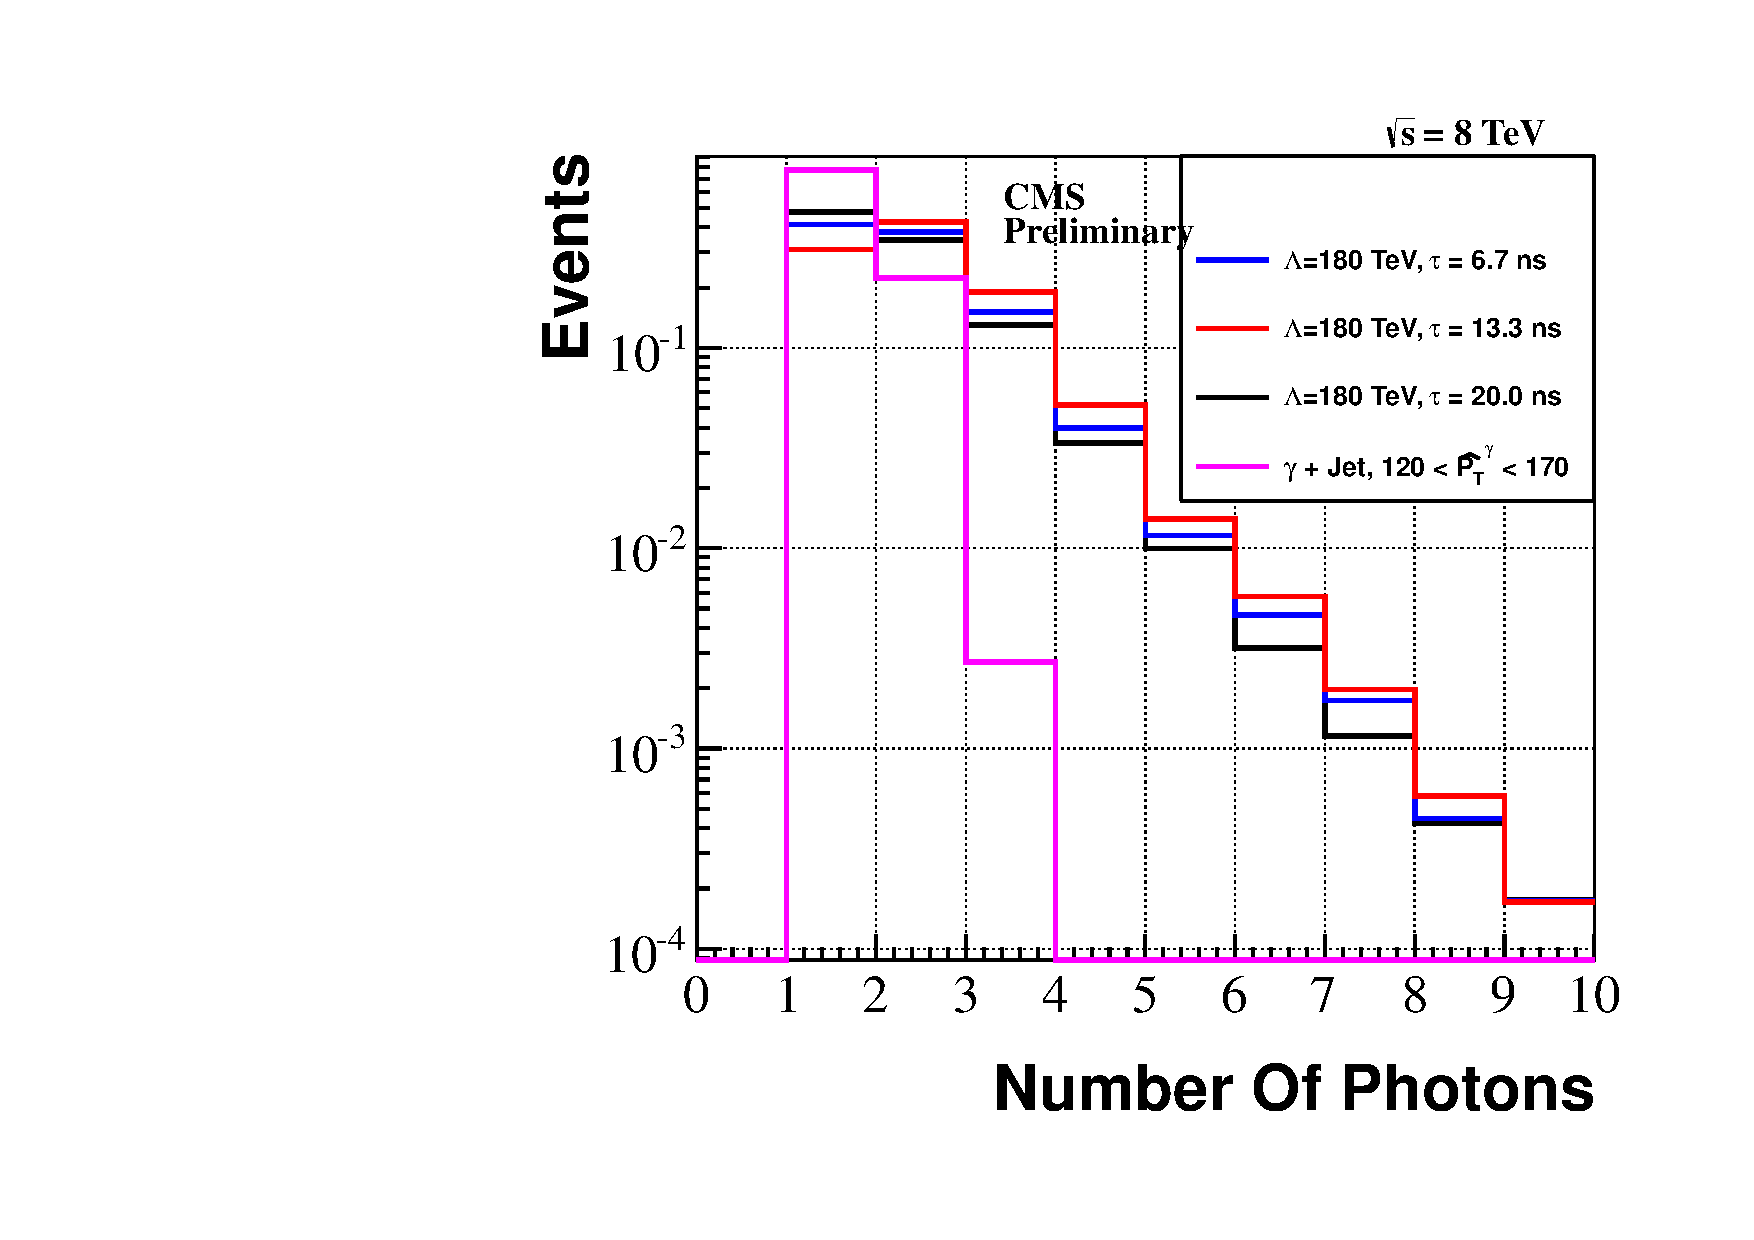
\includegraphics[height=0.6\textwidth,width=0.55\textwidth]{THESISPLOTS/GMSB-SPS8-MODEL-NumberOfPhotons_Lambda-180TeV.pdf}% \hspace{-1cm}
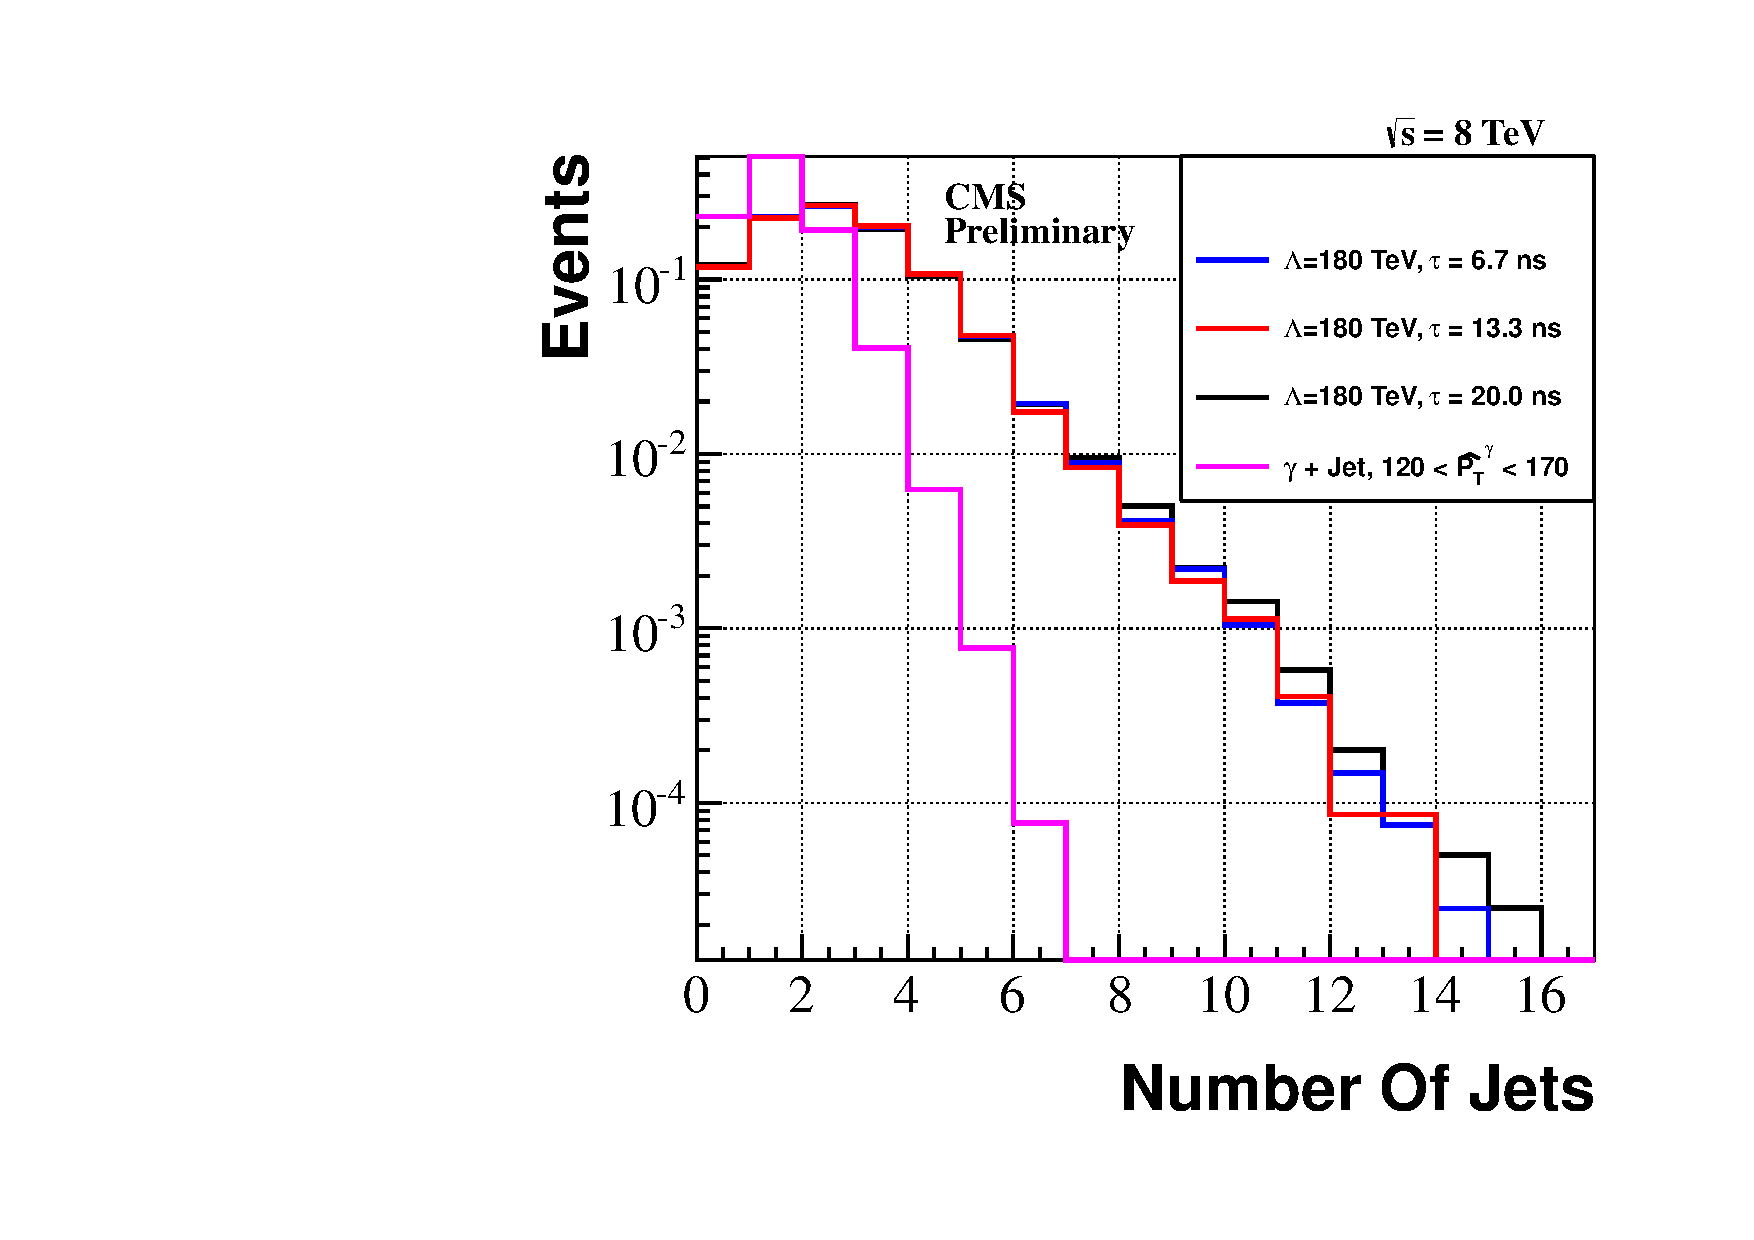
\includegraphics[height=0.6\textwidth,width=0.55\textwidth]{THESISPLOTS/GMSB-SPS8-MODEL-NumberOfJets_Lambda-180TeV.pdf}} \\
\hspace{0.5cm}
\mbox{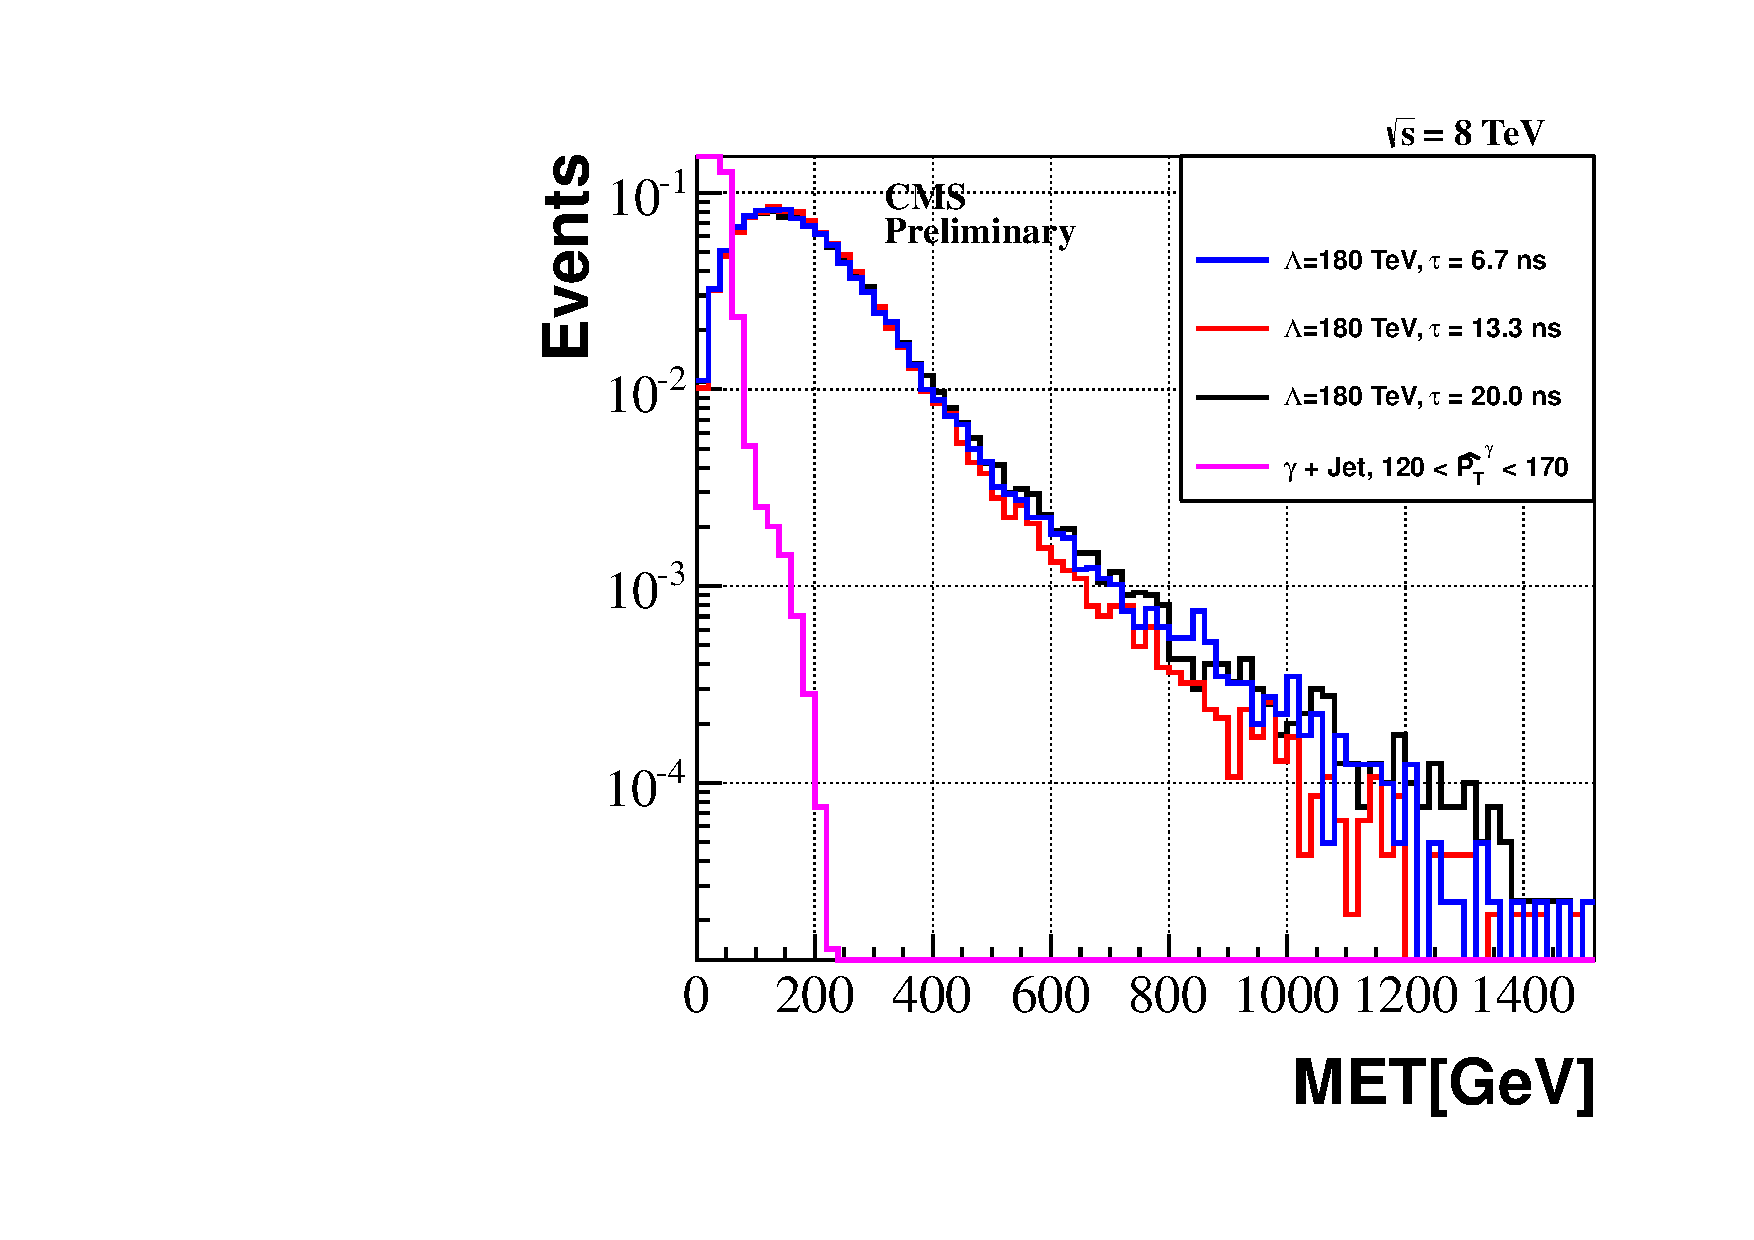
\includegraphics[height=0.55\textwidth,width=0.65\textwidth]{THESISPLOTS/GMSB-SPS8-MODEL-MET_Lambda-180TeV.pdf}}
\captionof{figure}{Number of photons with photon $\pt > 50\GeVc$~(top left), number of jets~(top right) and \MET~(bottom) for events with \PSneutralinoOne decay to $\gamma$ and $\tilde{G}$ for different lifetimes $\tau=6.7\ns,13.3\ns, 20.0\ns$ and $\mathbf{\Lambda} = 180$\TeV of the SPS8 benchmark GMSB model. A $\gamma +$jet with $120 < \hat{\pt} < 170$\GeVc sample shown for comparison with the signal samples.}
\label{fig:NKINE}
\end{center}
\end{minipage}

\subsection{Lifetime of the Lightest Neutralino}
The probability for a lightest neutralino~($\PSneutralinoOne$) with mass, $m_{\PSneutralinoOne}$, produced with energy, $\mathrm{E}_{\PSneutralinoOne}$, to travel a distance less than $x$ in the laboratory frame before it decays is
$\displaystyle{\mathcal{P}(x) = 1 - \exp{\left(- \frac{x}{\mathrm{L}} \right)} }$, where $\mathrm{L}$ is given as
\begin{equation}{\label{eq:decaylength}}
\mathrm{L} = \left(c\tau_{\PSneutralinoOne}\right) \cdot \left( \gamma \beta\right) = \left(c\tau_{\PSneutralinoOne}\right) \cdot \left( \frac{p}{m_{\PSneutralinoOne}}\right).
\end{equation} 
The distance traveled in the CMS detector by the \PSneutralinoOne before it decays depends on two main factors: the boost factor, $\left(\beta\gamma\right)_{\tilde{\chi}^{0}_{1}} = \frac{|\vec{p}_{\PSneutralinoOne}|}{m_{\PSneutralinoOne}} = \sqrt{\left(\frac{E_{\PSneutralinoOne}}{m_{\PSneutralinoOne}}\right)^{2} - 1}$, which indicates how fast the neutralino is traveling before it decays and the inherent  lifetime, $c\tau_{\PSneutralinoOne}$, of the \PSneutralinoOne. Slow moving \PSneutralinoOne have $\left(\beta\gamma\right)_{\tilde{\chi}^{0}_{1}} \ll 1$. Both factors determine the sensitivity of the ECAL to detect late photons from the decay of \PSneutralinoOne.
\newline
First, large values of $c\tau_{\PSneutralinoOne}$ means the distance traveled by \PSneutralinoOne is large and if larger than the ECAL radius which is about 1.3\m, \ie the \PSneutralinoOne traveled outside the ECAL volume before it decays, then detecting the delayed photon is no longer possible and this results to a loss in sensitivity by the ECAL. On the other end, small values of $c\tau_{\PSneutralinoOne}$, $c\tau_{\PSneutralinoOne} < 10\cm$, means the \PSneutralinoOne decays early and the photon is not late enough such that its detection using only ECAL timing measurements is not reliable and this once again results to loss in sensitivity by ECAL.
\newline
Second, lightest neutralinos~(\PSneutralinoOne s) produced with small momentum($p$) are less boosted and travel slow enough for their decay to happen inside the ECAL volume and the delayed photon is detectable using ECAL timing measurements which results to gain in sensitivity by ECAL. On the other hand, \PSneutralinoOne s produced with large momentum($p$) are highly boosted and travel out of the ECAL volume before they decay. Photons from such decays are not detectable and this also results to loss in sensitivity. In Figure \ref{fig:NKINE}, we show a distribution of the momentum of the \PSneutralinoOne in the transverse~($x-y$) plane~(transverse momentum~( $\pt^{\PSneutralinoOne}$)), the  transverse distance traveled by \PSneutralinoOne before it decays, the transverse momentum of the photon~($\pt^{\Pphoton}$) and photon's estimated time~($T_{\Pphoton}$) using only the event generator level information. 

\vspace{5mm}
\begin{minipage}{0.95\linewidth} 
\begin{center}
\mbox{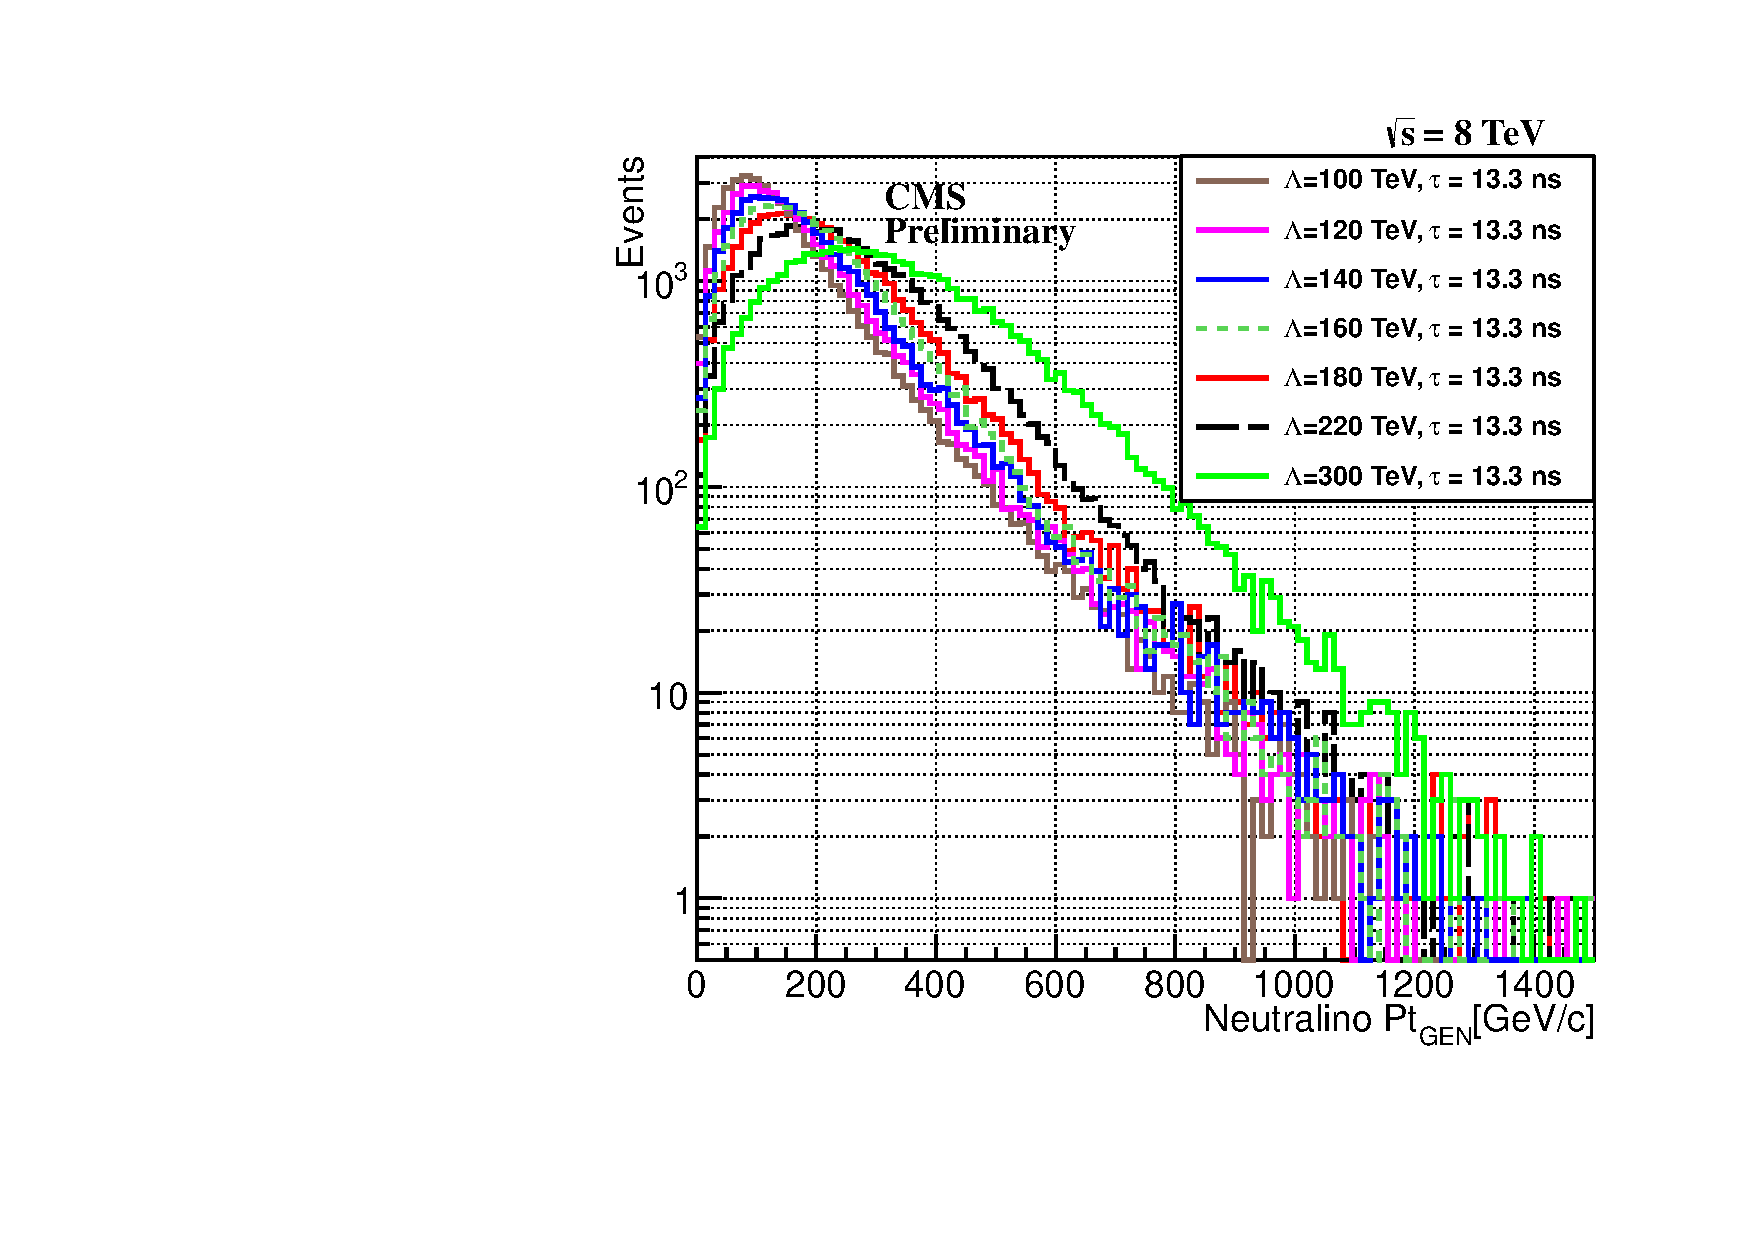
\includegraphics[height=0.60\textwidth,width=0.55\textwidth]{THESISPLOTS/GMSB-SPS8-MODEL-Neutralino-Pt_ctau-4000-mm.pdf} %\hspace{-1cm}
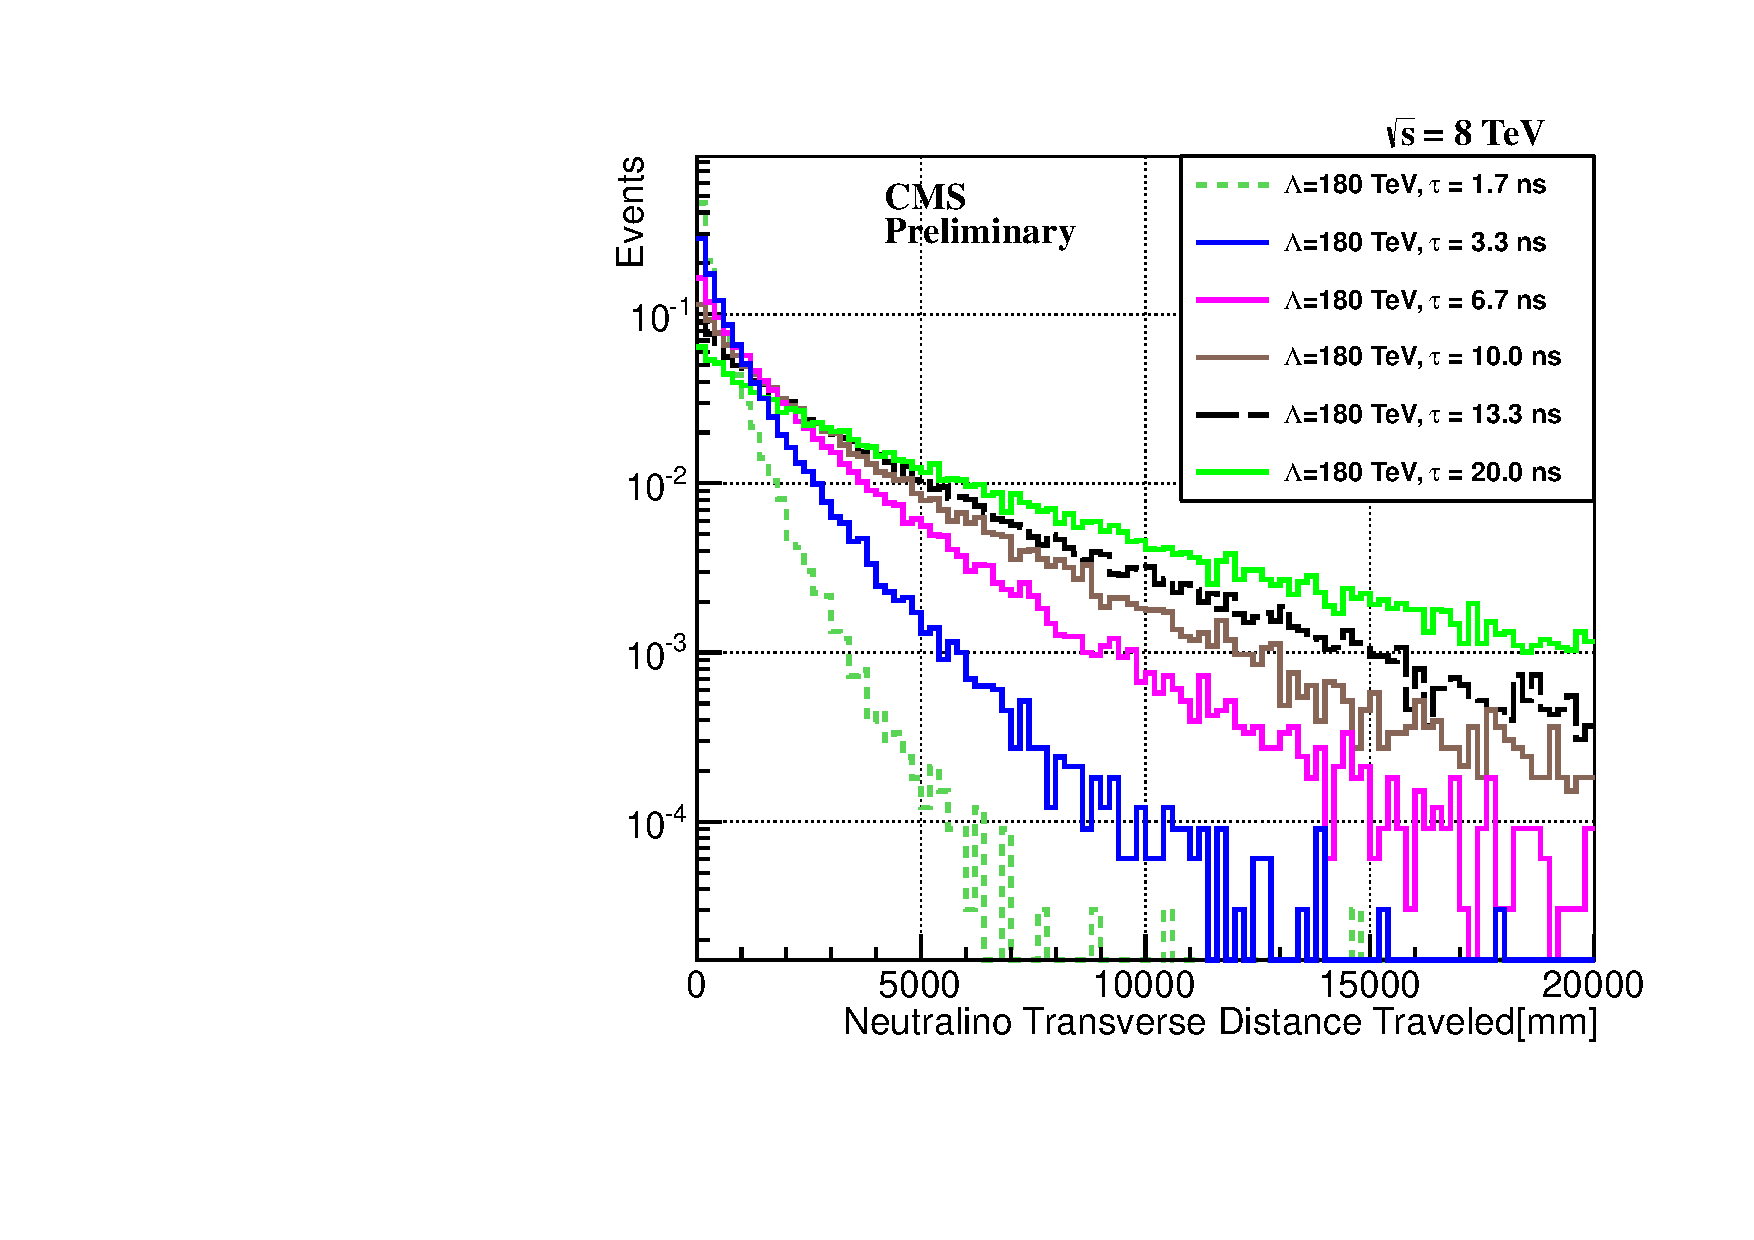
\includegraphics[height=0.60\textwidth,width=0.55\textwidth]{THESISPLOTS/GMSB-SPS8-MODEL-Neutralino-Proper-DecayLength_Lambda-180TeV.pdf}} \\
\hspace{0.5cm}
\mbox{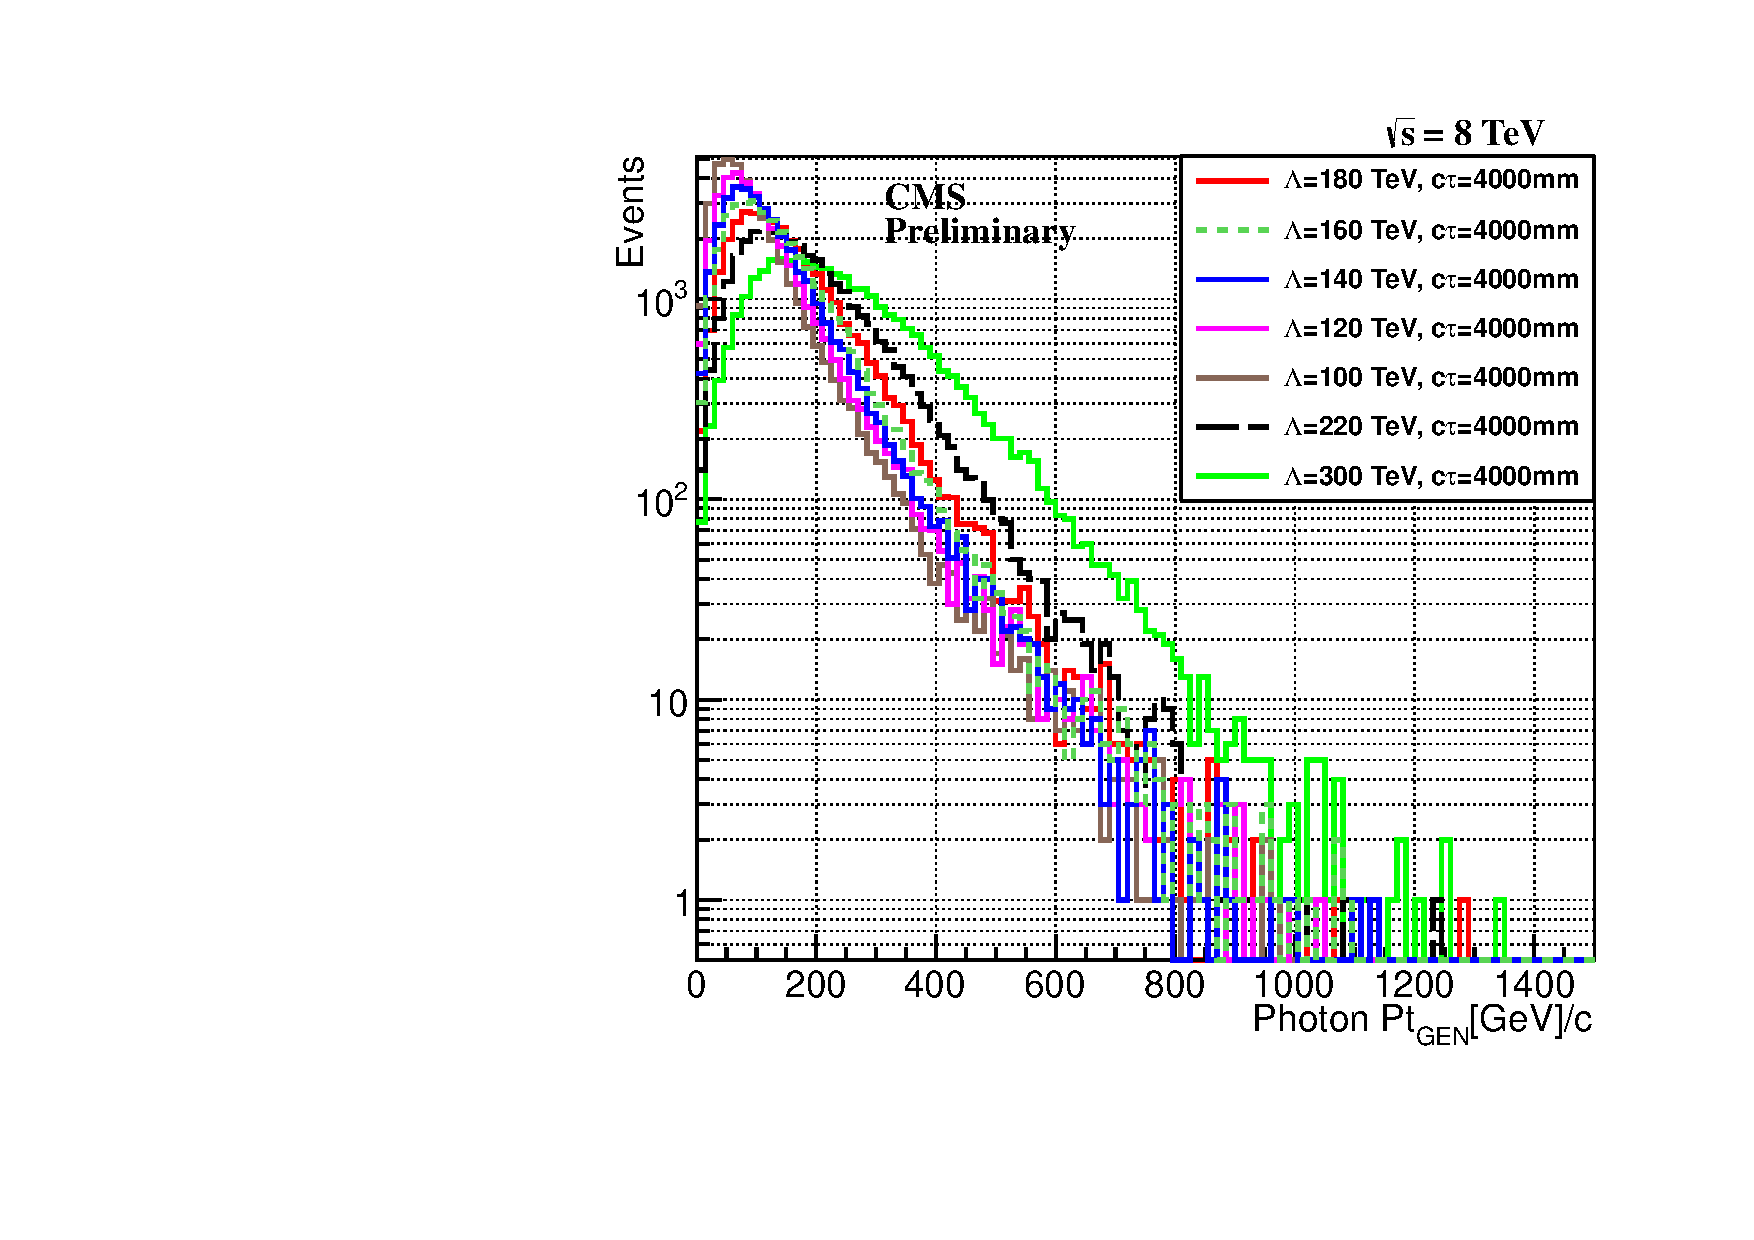
\includegraphics[height=0.60\textwidth,width=0.55\textwidth]{THESISPLOTS/GMSB-SPS8-MODEL-Photon-Pt_ctau-4000-mm.pdf} %\hspace{-1cm}
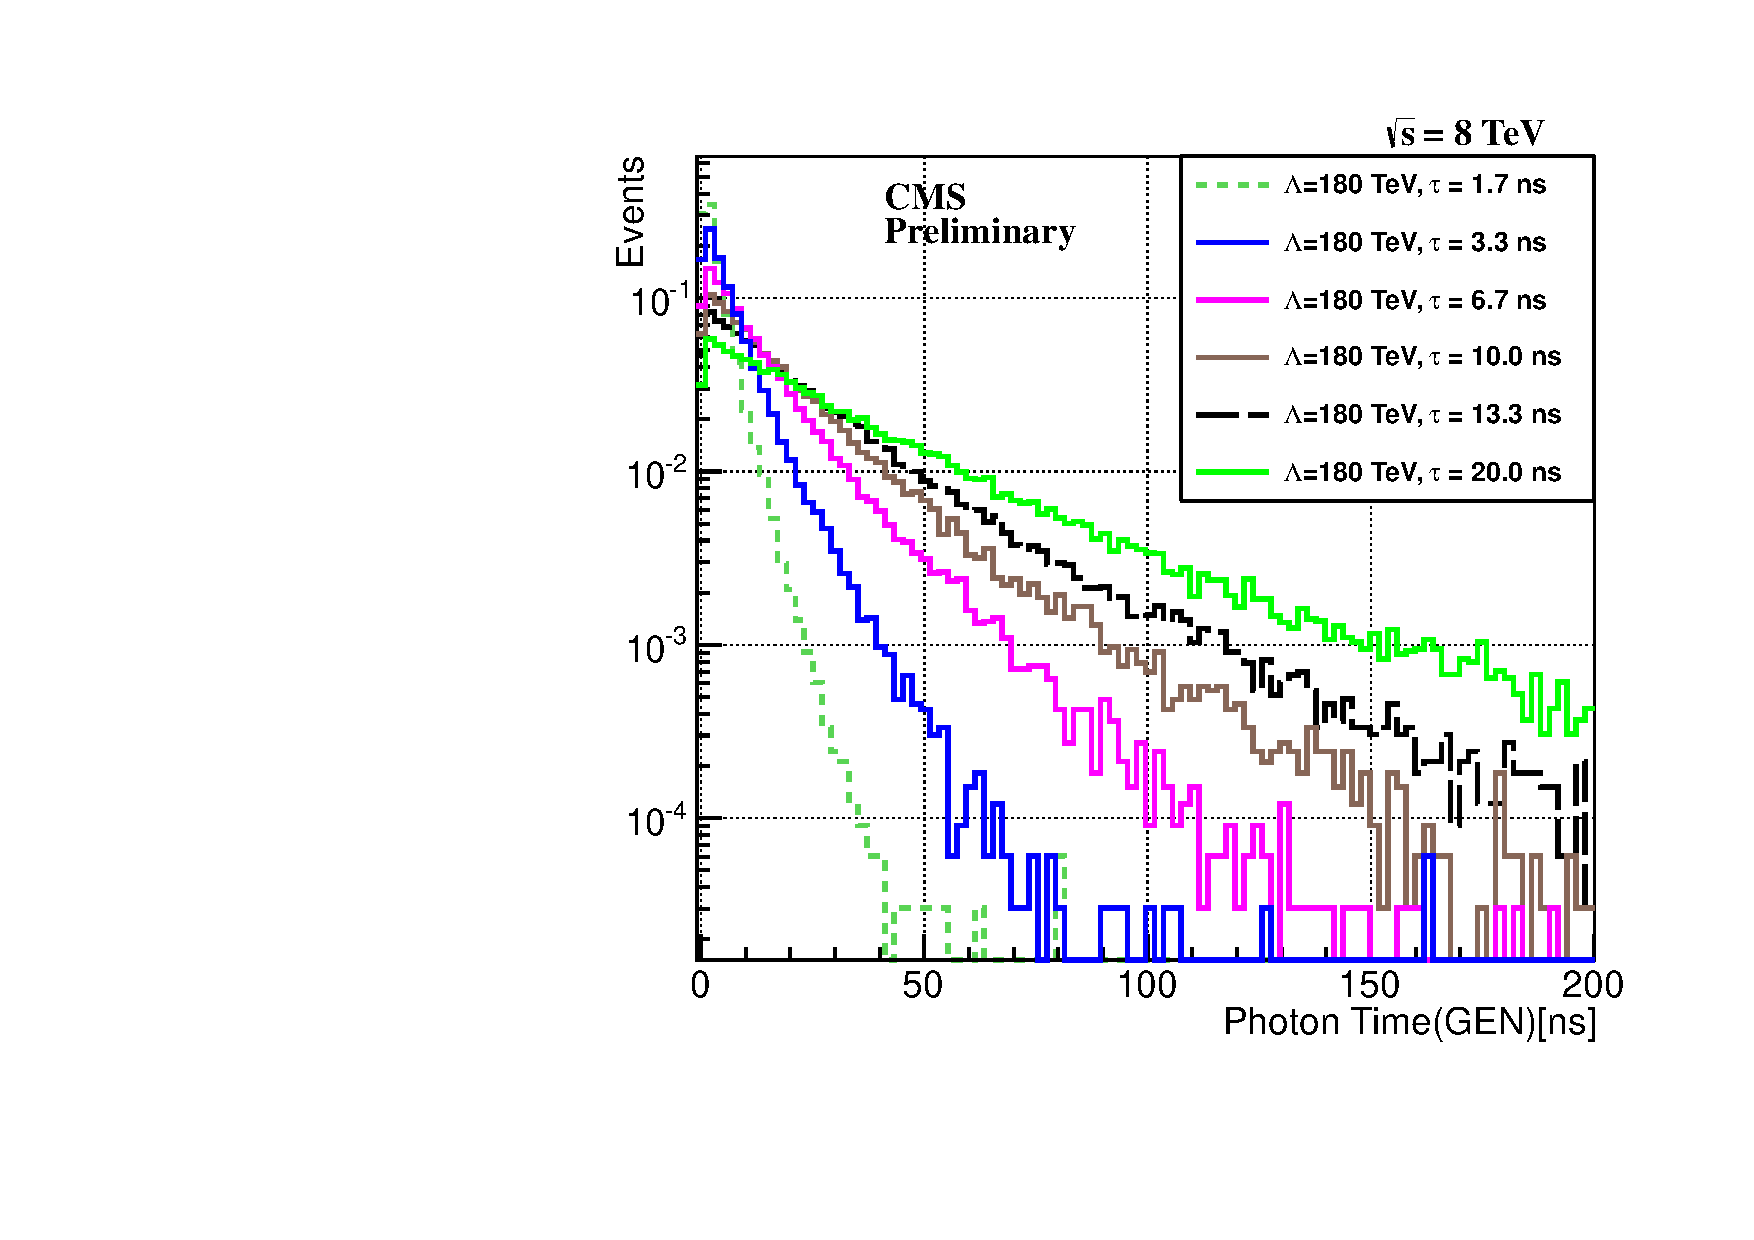
\includegraphics[height=0.60\textwidth,width=0.55\textwidth]{THESISPLOTS/GMSB-SPS8-MODEL-Photon-GEN-Time_Lambda-180TeV.pdf}}
\captionof{figure}{Neutralino transverse momentum~($\pt^{\PSneutralinoOne}$) distribution~(top left) and transverse distance traveled~(top right). Transverse momentum~(bottom left) and time~(bottom right) of photon from neutralino decay for different $\mathbf{\Lambda}$ and $c\tau$ points.}
\label{fig:NKINE}
\end{center}
\end{minipage}
 
%%\subsubsection{Source of Delayed Photons}
\vspace{5mm}
These distributions are for different $\mathbf{\Lambda}$ and $c\tau_{\PSneutralinoOne}$ points of the SPS8 benchmark GMSB model. We find that $\pt^{\PSneutralinoOne}$ increases with $\mathbf{\Lambda}$, from $\mathbf{\Lambda} = 100\TeV$ to 220\TeV. This is because as $\mathbf{\Lambda}$ increases the masses of the gluino/squark also increases and so does $\pt^{\PSneutralinoOne}$ since the \PSneutralinoOne is produced from the decay of the gluino/squark. In a similar argument, increasing the mass of \PSneutralinoOne ~($m_{\PSneutralinoOne}$) through increasing $\mathbf{\Lambda}$ leads to increase in the photon \pt. For a given value of $\mathbf{\Lambda} = 180\TeV$, which means the $\pt^{\PSneutralinoOne}$ is fixed, the transverse distance traveled by the \PSneutralinoOne before decay~(shown in the top right plot of Figure \ref{fig:NKINE}) and photon time~(shown in the bottom right plot of the same figure) increases with increasing value of the mean lifetime of \PSneutralinoOne from $c\tau = 500\mm~(\tau = 1.7\ns)$ to $6000\mm~(\tau = 20.0\ns)$. These observations support our expectation that the photon is delayed primarily due to the long lifetime  or distance traveled by the \PSneutralinoOne before it decays. 
\newline
The photon from the decay of \PSneutralinoOne can arrive late at ECAL for either one of the following reasons: first, because the \PSneutralinoOne is traveling slow \ie with boost, $\beta = \frac{p_{\PSneutralinoOne}}{m_{\PSneutralinoOne}} \ll 1$, and second, because the \PSneutralinoOne is produced with significant boost in the forward direction such that the photon travel to ECAL through a non-direct flight path from the nominal $pp$ interaction point. We study these two scenarios of the photon delay by estimating the photon arrival time at ECAL in each scenario using the  distance traveled by \PSneutralinoOne before it decays and the distance traveled by the photon from the decay point to ECAL. Figure \ref{fig:DELAY}~(left) shows a schematic representation of possible flight paths of the photon to ECAL. The estimated photon arrival ECAL time in each scenario is given as follows:
\begin{itemize}
  \item Delay due to slow moving neutralinos: $\Delta t_1$ = (L1/c$\beta$) - (L1/c)
  \item Delay due to non-direct traveled flight path: $\Delta t_2$ = (L1 + L2 - L3)/c
  \item ECAL  time recorded or measured = $\Delta t_{1} + \Delta t_{2}$
\end{itemize}
%\newline
\begin{minipage}{0.99\linewidth} 
\begin{center}
\mbox{
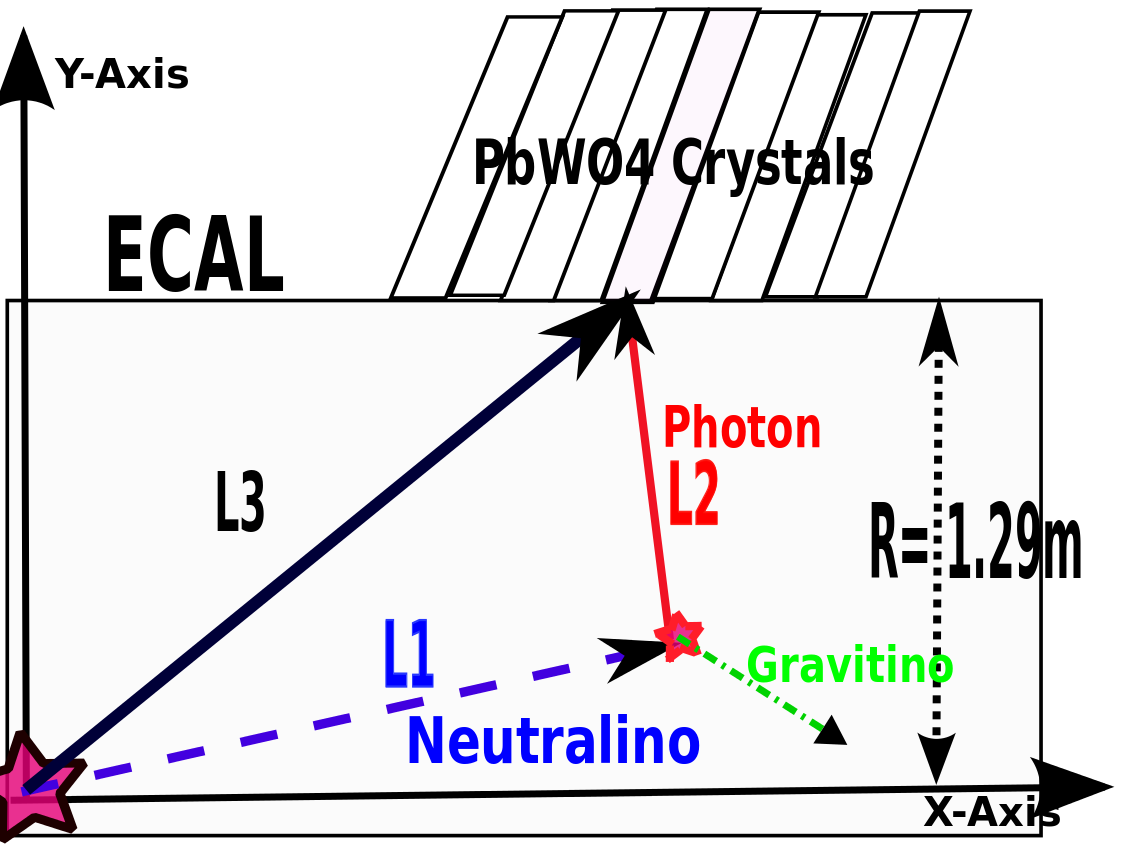
\includegraphics[height=0.55\textwidth, width=0.5\textwidth]{THESISPLOTS/DelayedPhoton-ECAL.png}
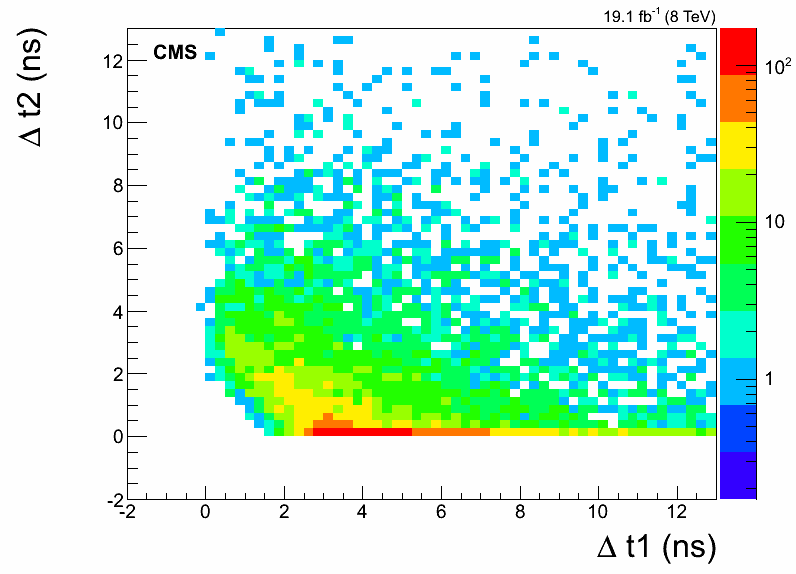
\includegraphics[height=0.55\textwidth, width=0.5\textwidth]{THESISPLOTS/dt1_dt2_late.png}
}
\captionof{figure}{Schematic diagram~(\textit{left}) of $\tilde{\chi}^{0}_{1} \rightarrow \gamma + \tilde{G}$ decay topology within the ECAL volume of the CMS detector. The estimated photon arrival time~(\textit{right}) at ECAL  from the decay of \PSneutralinoOne in the SPS8 benchmark GMSB model with $m_{\PSneutralinoOne}=256$\GeVcc and $\tau = 20\ns$.}
\label{fig:DELAY}
\end{center}
\end{minipage}

\vspace{5mm}
The \PSneutralinoOne is traveling with velocity, $v = c\beta$, where $c$ is the speed of light in vacuum. The distribution of the estimated delay in the photon arrival times due to the two sources, $\Delta t_{1}$ and $\Delta t_{2}$, is shown in Figure \ref{fig:DELAY}(right), where the color intensity represents the photon population. We find that most of the late arrival time photons are from the decay of slow moving \PSneutralinoOne compared to those from non-direct flight path of the photon to ECAL. This proves that when $c\tau$ is not so small a good number of \PSneutralinoOne s which are produced with low momentum such that the ratio $\frac{p_{\PSneutralinoOne}}{m_{\PSneutralinoOne}} \ll 1$, produces most of our detectable delayed photons using ECAL timing measurements. On the other hand, very long lifetime~($c\tau$) \PSneutralinoOne s which are produced with high momentum will very likely produce photons which escape the ECAL unless the \PSneutralinoOne decays inside the ECAL volume and the photon from the decay  arrives at ECAL through a non-direct flight path.
%%%%%
%%%%%%%%%%%%%%%%%%%%%%%%%%%%%%%%%%%%%%%%%%%%%%%%%%%%%%%%%%%%%%%%%%%%%%%%%%%%%%%%
%%%%%%%%%%%%%%%%%%%%%%%%%%%%%%%%%%%%%%%%%%%%%%%%%%%%%%%%%%%%%%%%%%%%%%%%%%%%%%%%
\section{Previous Search Experiments} \label{PrevResults}
%%%%%%%%%%%%%%%%%%%%%%%%%%%%%%%%%%%%%%%
There have been previous search experiments for events with delayed photons in their final state using the photon arrival time and missing transverse energy. Most~(except CMS which searched for events with  at least one photon) of these experiments searched for events with at least two photons in the final state and interpreted their results in the context of the SPS8 benchmark GMSB model. The results shown in Figure \ref{fig:UpperLimits} are from \DZERO, CDF, CMS and ATLAS \cite{LEP,CDF,ATLAS, CMS, ATLAS1} experiments and they present the excluded regions~(shaded) in the mean lifetime~($c\tau_{\PSneutralinoOne}[\mm]$ or $\tau_{\PSneutralinoOne}[\ns]$) and effective SUSY breaking scale~($\Lambda[\TeV]$) or mass~($m_{\PSneutralinoOne}[\GeVcc]$) of the lightest neutralino~(\PSneutralinoOne) in the decay, $\PSneutralinoOne \rightarrow \gamma + \tilde{G}$. Figure \ref{fig:UpperLimits}~(left) is produced from the search on data recorded by the ATLAS detector during $pp$ collisions at a center of mass energy, $\sqrt{s} = 7$\TeV while Figure \ref{fig:UpperLimits}~(right) is from \DZERO, CDF, CMS experiments with $p\bar{p}$ collision at $\sqrt{s} = 1.9$\TeV for \DZERO and CDF and $pp$ collision at $\sqrt{s} = 7\TeV$ for CMS. 
\newline
The important message from the results of these experiments is that within the SPS8 benchmark GMSB model, \PSneutralinoOne~s with mass, $m_{\PSneutralinoOne} \leq 245$\GeV, and mean lifetime, $\tau_{\PSneutralinoOne} \leq 3$~ns, are excluded at hadron colliders with the excluded region in $\tau_{\PSneutralinoOne}$ and $m_{\PSneutralinoOne}$ shrinking as the effective SUSY breaking scale, $\Lambda$, increases.

%%%%%%%%%%%%%%%%%%%%%%%%%%%%%%%%%%%%%%%
\begin{minipage}{0.99\linewidth} 
\begin{center}
\centering
\mbox{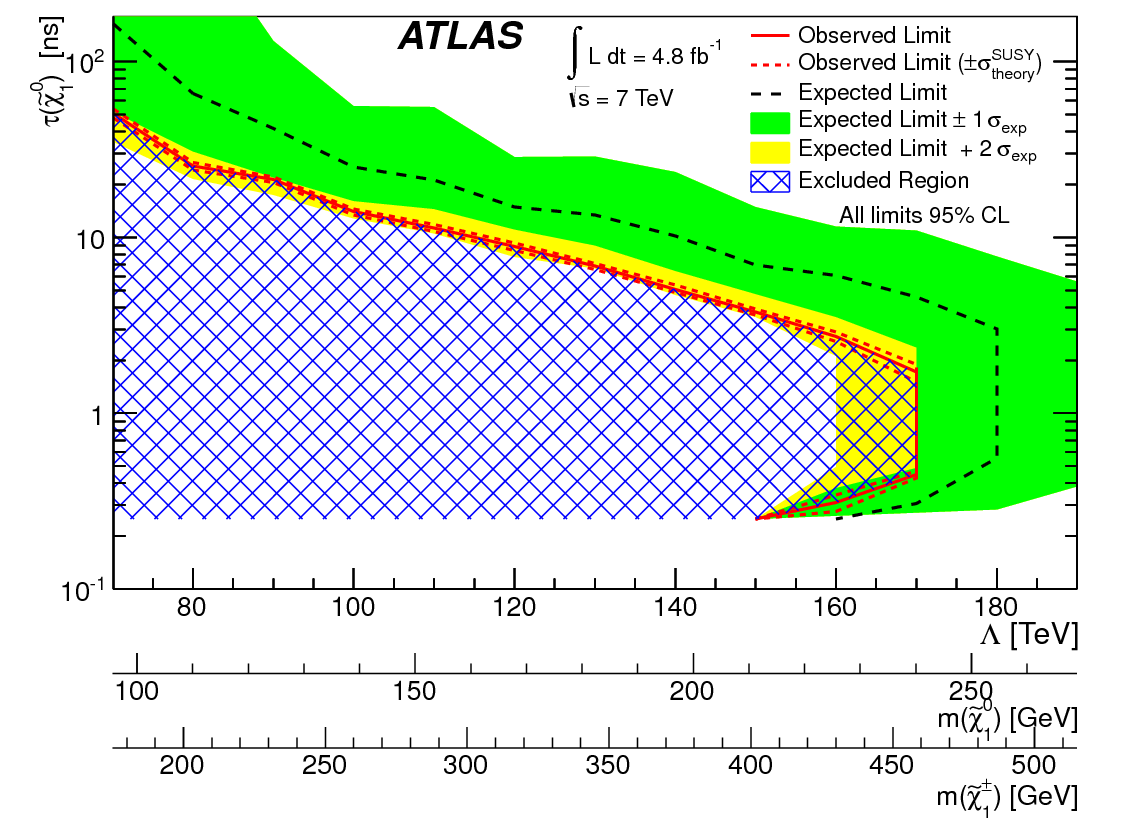
\includegraphics[height=0.7\textwidth,width=0.5\textwidth]
{THESISPLOTS/ATLAS_Upper_Limit.png}
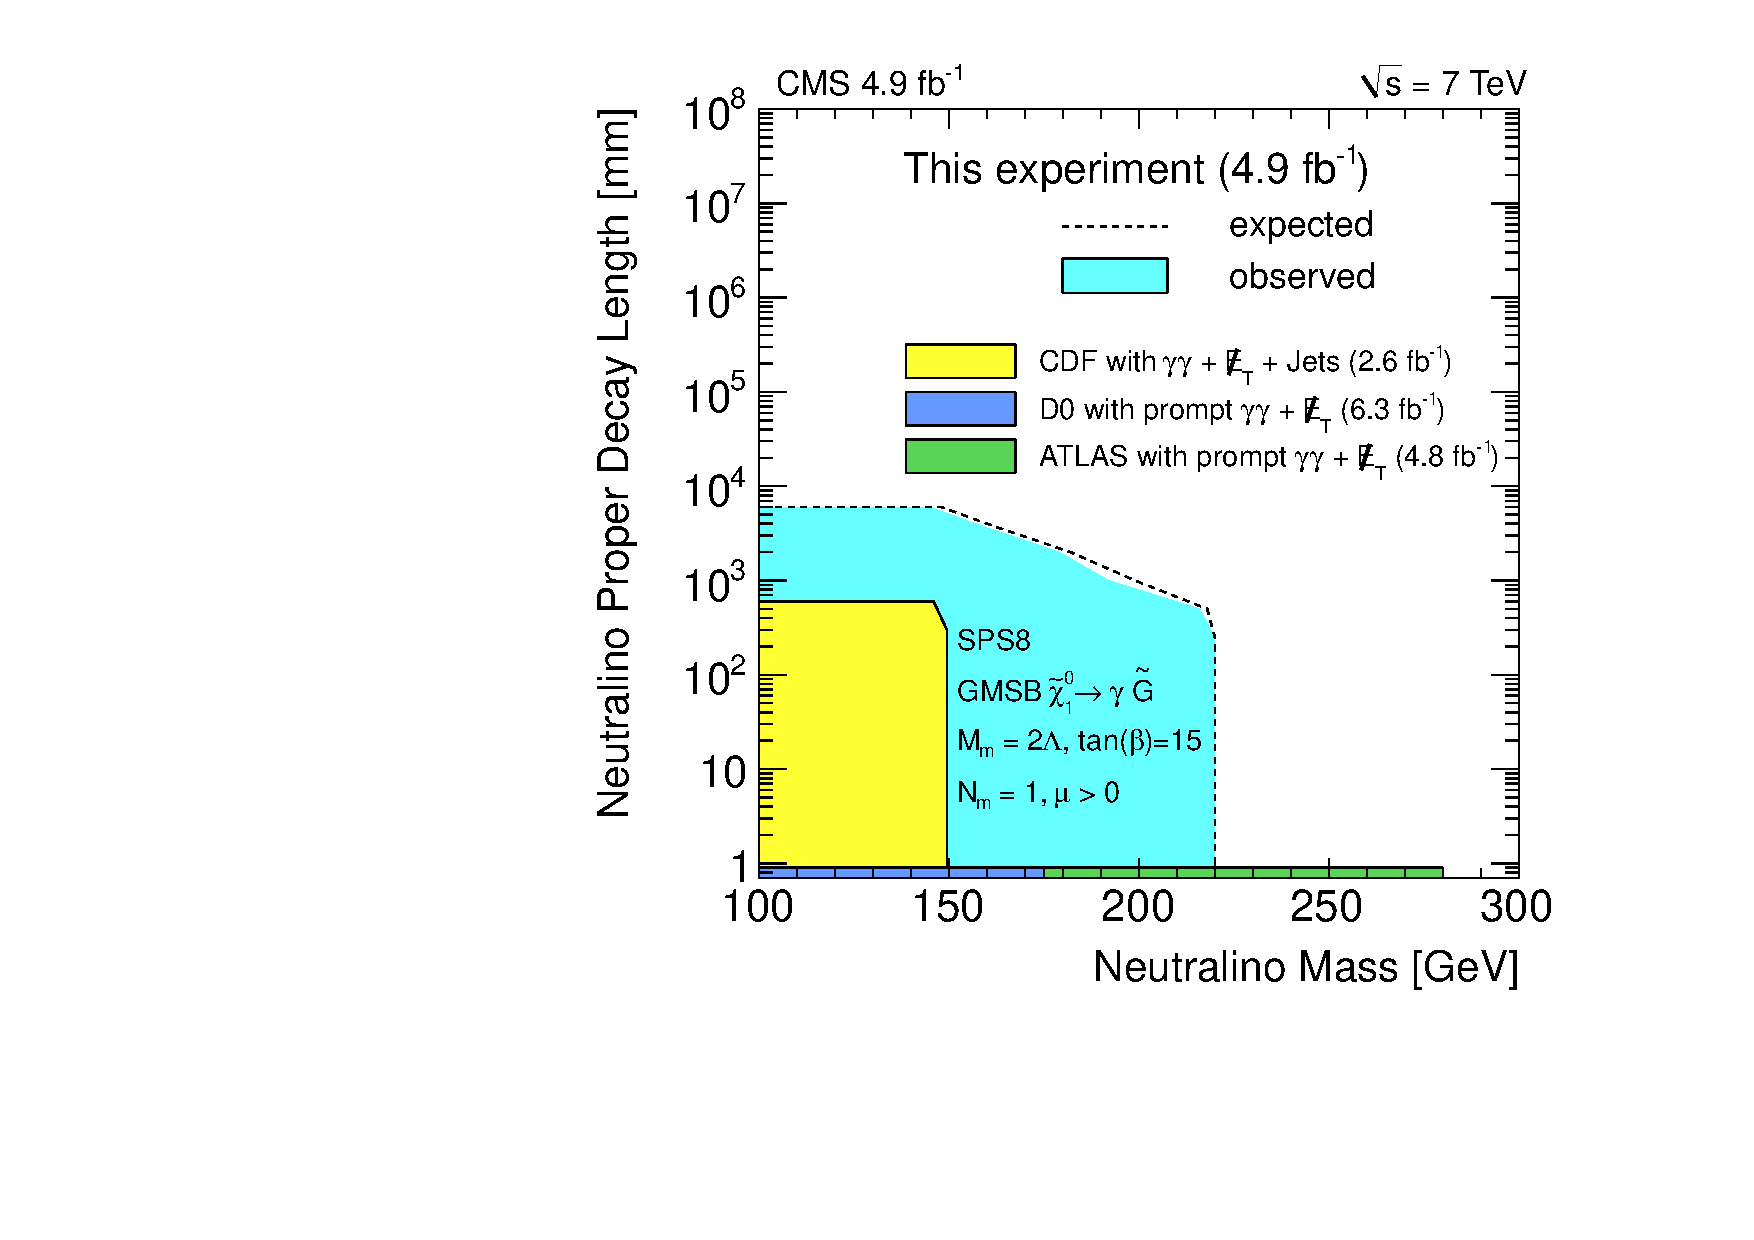
\includegraphics[height=0.73\textwidth,width=0.55\textwidth]{THESISPLOTS/2D_exclusion.pdf}}
\captionof{figure}{Neutralino lifetime and mass upper limit from ATLAS~(left) and CMS~(7\TeV), \DZERO and CDF experiments~(right) from the search for events with delayed or non-pointing photons.}
\label{fig:UpperLimits}
\end{center}
\end{minipage}

\vspace{5mm}

%%%%%%%%%%%%%%%%%%%%%%%##################### First written Section %%%%%%%%%%%%%%%%%%%%%
%%%%%%%%%
%These fundamental components or particles can be classified according to their \textit{spin} degree of freedom. A particle's spin~($s$) is an \textit{internal quantum number} expressed as $n\hbar$, where $n$ is either an \textit{integer} or \textit{half-integer}. Particles with half-integer spins are called \textit{fermions} while those with integer spins are called \textit{bosons}. In the SM, fermions and bosons obtain their mass from interaction with a Higgs boson through a spontaneous symmetry breaking process. 
%\newline
%The Standard Model~(SM) of particle physics provides a thorough and experimentally verified mathematical description of the fundamental constituents of visible matter and their interactions~(except gravity) in the universe. Predictions of particle properties and interactions by the SM agree with most of the available experimental data with unmatched precision.
%However, despite the success of the SM, there are some theoretical and experimental inconsistencies with the SM, such as the indirect observation of Dark Matter~(DM) in the universe which cannot be described by the SM, the observation of neutrino oscillations and neutrino masses unexplained by the SM and the absence of gravity in the SM. These limitations of the SM forces many physicists to believe that the SM could be part of a more general model describing all the phenomenons observed in the universe. \textit{supersymmetery}~(SUSY) is among many Beyond Standard Model~(BSM), a theoretical extension of the SM to address these limitations. Before, we proceed with discussing SUSY and how it addresses the limitations of the SM, we first introduce some of the concepts in the SM which are common in SUSY.



%%% Terrible parts
% produced from the cascade decay of squarks and gluinos can decay into a gravitino and a gauge boson or scalar particle. This decay is also a probabilistic process and can be expressed and quantified as a single real number. 
% There are always many options for a given particle to decay into and each of these options is quantified by a number known as the \textit{Branching  Fraction} or \textit{Branching Ratio}. Summing all the branching ratios for all the different decay processes gives the total \textit{Decay Width}. The total decay width, can also be computed and expressed as a single real number in units of \GeV or \MeV (\GeV = giga electron volt $=10^{9}$~eV). 
 %In the case of the neutralino as the NLSP, the decay width depends on the nature of its interaction with the gravitino and an associated gauge boson or scalar field.
%\paragraph*{}


%\newline
%We describe briefly, in the next sections, the major components of the SM along with its strengths and limitations and also introduce SUSY as the most studied BSM.

%Mass, charge, spin and lifetime can be used to identify and categorize fundamental particles of nature.
%Particles with the same charge, mass and spin but with the opposite charge are called \textit{anti-particles} while particles with equal proportion of positive and negative charges are said to be neutral. An interesting classification of particles and anti-particles can be made using their \textit{spin}~($s$).


%\subsection{Limitations of the Standard Model }
%%Although numerous experiments agree with SM predictions of particle properties with unmatched precision, there are many unanswered questions by the SM. The following are some  of the questions we considered interesting.
%~(Glashow, 1961; Weinberg, 1967; Salam, 1968) describes almost entirely all of the observed phenomena and fundamental particles of nature with unmatched precision.
%However, more concerning our universe is yet to be understood. A few of this include:
%%\begin{itemize}
%%\item \textbf{General Formalism} \mbox{}\\ There are important parameters like particle masses, Weinberg angle, the CKM matrix elements, for example, which cannot be derived from the SM. These parameters can only be measured from experiments. Questions like why are there only 3 generations of particles?  why only one Higgs doublet in the SM, are unanswered by SM.
%The Electro-weak symmetry breaking which is central to the SM is not very well understood as the SM does not provide an explanation of whether there are more than one spin-0 boson responsible for particles masses or not.

%%\item \textbf{Cosmological} \mbox{}\\
%%Why is there so much matter than anti-matter in the universe? \textit{Cosmic Microwave Background}~(CMB) and the \textit{Wilkinson Microwave Anisotropy Probe}~(WMAP) experimental results indicate the presence of excess matter which does not interact with light called \textit{Dark Matter}~(DM) and \textit{Dark Energy}~(DE). DE is responsible for the increase energy density causing rapid accelerating expansion  of the universe. The nature of DM and DE and such observations cannot be explained using the current SM.
%If the Big Bang theory which describes the creation and existence of the universe is assumed to be the correct theory, then matter and anti-matter should be observed in equal composition. However, astrophysical measurements of the ratio of barons to anti-baryons referred as the \textit{Baryon asymmetry ratio} shows that there is more matter than anti-matter in the universe. Where is all the expected anti-matter? This could fairly be explained through charge-parity violation in weak interactions of the SM but this contribution is not enough to explain the entire observed baryonic matter discrepancy. Observations through \textit{Baryonic Acoustic Oscillation}~(BAO) or .
%%\item \textbf{Theory} \mbox{}\\
%%SM description of nature does not include gravitational interactions.
%%Observation of SM coupling constants varying with energy begs the question of whether at a higher energy scale, all the weak, strong and electromagnetic forces start to behave as a single force i.e unification of all the different coupling constants as a single coupling constant. If this is possible, what is the energy scale where this force unification happens?

%%\item \textbf{Mass Hierarchy or Naturalness} \mbox{}\\
%%Particle masses range from neutrino masses of a few eV to the \textsf{top} particle's mass of 173~\GeVcc. This observed mass hierarchy cannot be explained by the SM.
%%To some physicist, the energy gap between the electro-weak symmetry breaking energy scale~( $\approx 246$~\GeV) and the Planck energy scale~(reduced Planck mass, $M_{p} = 10^{18}$~\GeV) seems unnatural.

% The SM only accounts for how particles obtain their mass through their interaction with a scalar field~(spin-0), the Higgs boson. However, the experimental observation of this particles mass hierarchy is not understood. Infact according to the SM, neutrinos have no mass. 
%From an energy scale point of view, this lack of our understand also known as the \textit{hierarchy} "\textit{problem}" can be posed as follows; why do experiments observed such a 
%A consequence of this, is on the experimentally observed value of the mass of the Higgs boson, $\approx 125$~\GeV. The Higg's mass is stable and does not grow to very large values as the energy scale increases towards $M_{p}$ as one would expect from theoretical calculations.  \textit{Supersymmetry}, an extension of the SM, allowing for the possibility of more than a single Higgs boson, provides an explanation for why the  Higg's mass remains stable at all energy scale. Its main idea, is the existence of fundamental new particles with masses within the weak and gravity energy scale and through their interaction with the higgs keeps its mass stable. We will see more of this in the next section.
%%\end{itemize}

%The entire components of this matrix is measured from experiment and not derived from the SM.
%%\clearpage

%%\vspace{5mm}
%%\begin{minipage}{0.90\linewidth}
%%\begin{center}
%%\centering
%%\bfseries{Particle and Their Gauge Symmetry Representation}
%%\begin{tabular}{c|c|c|c}
%% \toprule
%%\bfseries{Particle Name(Symbol)} & \bfseries{Spin} & \bfseries{Multiplet} & \bfseries {$SU(3)_{C} %%\otimes SU(2)_{L} \otimes U(1)_{Y}$}\\
%%\hline\hline
%% Quarks ($Q$) & 1/2 & $(\Pup_{L}, \Pdown_{L})$  & $(\mathbf{3}, \mathbf{2}, \frac{1}{6})$\\
%% $\bar{\Pup}$ & 1/2 & ${\Pup^{\dagger}_{R}} $& $(\mathbf{\bar{3}}, \mathbf{1}, -\frac{2}{3})$\\
%% $\bar{\Pdown}$ & 1/2 & ${\Pdown^{\dagger}_{R}} $& $(\mathbf{\bar{3}}, \mathbf{1}, \frac{1}{3})$\\
%% ($\times 3$ families) & & & \\
%%\hline
%% Leptons($L$) & 1/2 &  $(\Pnu, \Pe_{L} )$ & $(\mathbf{1}, \mathbf{2}, -\frac{1}{2})$\\
%% $\bar{\Pe}$ & 1/2 & ${\Pe^{\dagger}_{R}} $& $(\mathbf{\bar{1}}, \mathbf{1}, 1)$\\
%%% ($\times 3$ families) & & & \\
%% & 1/2 & $\Pneutrino^{\dagger}_{R}$ & $(\mathbf{\bar{1}}, \mathbf{1}, 1)$ \\
%%\hline
%%Higgs ($\PHiggs_{u} $) & 0 & $(\PSHiggsplus_{u}, \PSHiggszero_{u})$ &  $(\mathbf{1}, \mathbf{2}, +\frac{1}{2})$ \\
%%Higgs($\PHiggs_{d}$)   & 0 & $(\PSHiggsplus_{d}, \PSHiggsminus_{d})$ &  $(\mathbf{1}, \mathbf{2}, -\frac{1}{2})$ \\
%%\hline\hline
%%\bfseries{Force Carriers} &  & & \\
 %%Gluons & 1 & $\Pgluon$ & $(\mathbf{8}, \mathbf{1}, 0)$ \\
 %%(Strong Force) & & & \\
%% \hline
%% $\PW$ bosons & 1 & $\PW$ & $(\mathbf{1}, \mathbf{3}, 0)$ \\
%% $\PB$ boson & 1 & $\PBzero$ & $(\mathbf{1}, \mathbf{1}, 0)$ \\
%% (Electro-Weak Force) & & & \\
%%\hline 
%% \bottomrule
%%\end{tabular}
%%\captionof{table}{SM particles and their gauge multiplets(representation) with their quantum numbers.
%%The quantum numbers, for example, $(\mathbf{3}, \mathbf{2}, \frac{1}{6})$, means (\textit{triplet},\textit{doublet}, $Y = 1/6$) representation in each gauge symmetry. }
%%\label{tab:SM} 
%%\end{center}
%%\end{minipage}
%%\vspace{5mm}


%This decay rate depends on the mass of the gravitino $m_{\tilde{G}}$ as long as R-parity is conserved. Thus, in the decay of every MSSM particle, the gravitino will likely or eventually be included in its final states. We can  parametrised this decay rate by using $C_{grav}$. It is easy to see that $C_{grav} \geq 1$. It is important to note that there are other GMSB phenomenological observations which do not entirely considered the gravitino as the lightest supersymmetric particle.
%Thus in order to study the phenomenology of GMSB models, one can define a parameter space using the following parameters given in equation \ref{eq:mGMSB}. 
%\begin{equation}{\label{eq:mGMSB}}
%\left\{ \mathbf{\Lambda}, \quad \mathbf{M}_{\mbox{mess}},\quad \mathbf{N}_{5}, \quad \tan(\beta), \quad sgn(\mu),\quad C_{grav}\right\}
%\end{equation}
%These sets of parameters given in equation \ref{eq:mGMSB} are those we will be studying  within the minimal GMSB~(mGMSB).
% In other gauge mediating supersymmetry models like the General Gauge Mediation SUSY breaking~(GGM), $\left\{M_{3}(\mbox{gluino mass}), M_{2}(\mbox{Wino mass}), M_{1}(\mbox{Bino mass}),\tan(\beta), sgn(\mu), c\tau_{NLSP}\right\}$
%is the parameter space,\cite{GGM1,GGM2}.
%In GGM models, colored sparticles are not required to be heavier than their Electro-Weak sparticles allowing for greater discovery potential at hadron collider\cite{DSHIH}. Thus, allowing for possibility of many candidates NLSP particles and not only the neutralino as in the case with mGMSB models like the SPS8 model.
%For Pure General Gauge Mediation SUSY breaking~(PGGM), the parameter space is rather scan using $\displaystyle{\left\{\Lambda_{G},\Lambda_{S}, \mathrm{M}_{\mbox{mess}}\right\} }$ parameter set.
%Of all other possible decay modes in GMSB models, this thesis is interested only in decays where eventually, the Next-To-Lightest SUSY particle~(NLSP) decays to the lightest SUSY particle~(LSP) which is the gravitino and its SM partner; i.e if particle, $\tilde{p}$ is the NLSP, then it will decay is given according to equation \ref{eq:NLSPDECAY}.
%\begin{equation}
%%\tilde{p}\rightarrow p + \tilde{G}
%\end{equation}

%% SUSY rubbish stuff
%\vspace{5mm}
%\textit{Chiral} and \textit{Vector} superfields are used in constructing the minimal supersymmetric standard model.
%In relativistic Quantum Field Theory~(QFT), the idea of symmetry or group theory is used to provide a better understanding of fundamental particles and their properties. These symmetries belong to two broad categories: space-time symmetries known as Poincar\'{e}(i.e rotation and translation) symmetries and gauge ( such as $SU(3)_{C}\otimes SU(2)_{L}\otimes U(1)_{Y}$ with quantum numbers; color, weak and hypercharge respectively of the SM) symmetries. With the SM viewed as a low energy version of a more large and unified theory,  
%that all fundamental forces including gravity could be unified 
%In a quest to include gravitational interaction along with all the other forces of nature into a unique frame work called unification, 
%it was believed that combining these two classes of symmetries into one big class of symmetry could lead the way towards the development of this unified theory. However, Coleman and Mandula\cite{SUSY}, in their so-called "\textit{no-go}" theorem in 1967  showed that pursuing the approach of \textit{direct product} of the two super groups  was not possible. %Thus these two class of symmetries cannot be combined into a bigger parent symmetry. 
%The challenge was finding a scenario where the generators of both space-time $P^{\mu}$, $M^{\mu\nu} $  and gauge groups $T^{a}$, do not commute with each other; i.e $ \left[M^{\mu\nu}, T^{a}\right] \neq 0$ and yet remains a direct product of both symmetry groups, considering that the direct product of these groups do commute; i.e
%the generators of these groups; $P^{\mu}, M^{\mu\nu}$ and $T^{a}$ corresponding to these symmetries have a direct product;  Poincar\'{e} $\times$Gauge group, for which
%$ \left[P^{\mu}, T^{a}\right] = \left[M^{\mu\nu}, T^{a}\right] = 0$. 
%\newline
%This \textit{no-go} theorem prevents the possibility of finding a parent group where its generators are constructed from \textit{Lorentz} tensors. Thus, only symmetries  generated from \textit{spinoral}~(particle's spin) charges instead of \textit{tensorial}~(space-time) charges were possible. In 1975, Haag, Lapuszanski and Sohnius \cite{MSUSY} found such a group theorem known as the \textit{Haag-Lapuszanski-Sohnius} theorem with its corresponding generator algebra called the \textit{Lie-superalgebra} or the \textit{supersymmetry algebra}.  This supersymmetry algebra extended the commutative aspect of the Poincar\'{e} algebra to include \textit{anticommuting} symmetry generators.
%\newline
%\textit{Lie-superalgebra} generators, $\mathrm{Q}_{i}$, $i = 1,...,\mathrm{N}$, where $\mathrm{N}$ is the number of supersymmetry generators, anti-cummute with the group and space-time generators.  % as shown in equation \ref{eq:SUSYGEN}. 
%Supersymmetry is a well developed and advanced branch in theoretical physics where the number of supersymmetry generators can be any number. However, this thesis only considers the case where there is only one generator of supersymmetry; i.e $\mathrm{N} = 1$. This is the minimal  version of supersymmetry. 
% The generators $\mathrm{Q_{1}} \equiv \mathrm{Q^{\alpha}}$, where $\alpha=1,2$ is labeling \textit{Weyl or two spinor} components,  and its hermitian conjugate, $\mathrm{\bar{Q}_{\alpha}}$, must satisfy the relations given in equation \ref{eq:SUSYGEN}.
%\begin{eqnarray}{\label{eq:SUSYGEN}}             
%\left\lbrace\mathrm{Q_{\alpha}}, \mathrm{\bar{Q}_{\beta}}\right\rbrace =  2\left(\gamma^{\mu}\right)_{\alpha\beta}P^{\mu}, &
%\left[\mathrm{Q_{\alpha}},P^{\mu}\right] = 0, &
%\left[\mathrm{Q_{\alpha}}, M^{\mu\nu}\right] =\frac{1}{2}\left(\Sigma^{\mu\nu}\right)_{\alpha}^{\beta}\mathrm{Q_{\beta}}
%\end{eqnarray}
%$\gamma^{\mu}$ is define such that 
%Where $\left\lbrace \gamma^{\mu}, \gamma^{\nu}\right\rbrace = 2\mathrm{g^{\mu\nu}}$ and  $\Sigma^{\mu\nu} = \frac{i}{2}\left[\gamma^{\mu},\gamma^{\nu}\right]$ 
%. %and $\mathrm{\bar{Q}_{\alpha}}$ is the Hermitian conjugate to $\mathrm{Q}$.
%These relations in equation \ref{eq:SUSYGEN} reveal two very fundamental consequences of supersymmetry:
%\begin{itemize}
%\item  Particles in a given state~(\textit{supermultiplet}) have the same mass but differ in their spin by half $\hbar$ unit.
%\item In every irreducible representation of supersymmetry, there is an equal number of fermionic and bosonic degrees of freedom. 
%\end{itemize}
%Thus, supersymmetry is the symmetry which transforms particles from one spin into another with the same mass. As a consequence, supersymmetry generators transform fermions into bosons and bosons into fermions with the same mass.
%This reveals that, in supersymmetry, 
% chosen such that every SM particle with spin 0,$\frac{1}{2}$, 1, 2 have a partner with spin $\frac{1}{2}$,0,$\frac{1}{2}$,$\frac{3}{2}$ respectively in the same supermultiplets.
%In addition to an algebraic approach to supersymmetry described so far, in order to build models~(supersymmetric Lagrangians) and make predictions, we return to the idea of fields as used in supersymmetry. Supersymmetric fields are called \textit{superfields}~( proposed and realized by Abdus Salam and Strathdee \cite{SALAM, SUSYBOOK}) are fields defined on a superspace; an ordinary Minkowski space-time, $x^{\mu}$ and four anti-commuting \textit{Grassmann} numbers, $\theta$. More on this can be seen in  \cite{SUSYBOOK}.
%These superfields are operator-valued functions, \textbf{$\Phi$}, on a superspace represented by, \textbf{$\Phi\left(x^{\mu},\theta,\bar{\theta}\right)$}.
%Its components consist of ordinary scalar fields~(real or complex), Lorentz vector fields and Left-handed or Right-Handed Weyl(2 degrees of freedom) spinor fields, \textbf{$\Phi\left(x^{\mu},\theta,\bar{\theta}\right) \supset (\phi, \psi, A_{\mu}, F)$}.
%Table \ref{tab:SUSYF} shows an example of the components which make up the  superfield~( or supermultiplets) with each component representing a SM particle and its super partner with the same mass. Only the Chiral and Vector  superfields are used in constructing the minimal supersymmetric version of standard model
%\begin{center}
%\centering
%\begin{tabular}{|c| c|}
%\mbox{Supersymmetry multipletes and spin }
%\hline
%\bfseries{Superfields or supermultipltes } & \bfseries {Component Fields}\\
%\hline
%\textit{Chiral} & $(\psi, \phi, F)$ \\
%\textit{Vector} & $(A_{\mu},\lambda, D)$ \\
%\textit{Gravity} & $ (G_{\mu\nu}, ... ) $ \\
%\hline \hline
%\end{tabular}
%\captionof{table}{Supermultiplets and components in Supersymmetry.}
%\label{tab:SUSYF} 
%\end{center}

%%% SM stuff
%This angle participates in an important phenomenon in SM known as quark mixing. Unfortunately in the current simplest state of SM, there are no lepton mixing(due to a global symmetry called lepton number conservation) even though the recent discovery of neutrino masses existence \cite{} hints at the possibility of such a mixing in the lepton flavour sector.
%Nevertheless, in the quark sector, it is possible for the $W^{\pm}$ to change the flavour of a given quark, for example and up-type quark u can transition to a down-type quark d. This type of transitions are referred to as Flavour Changing Charge Currents~(FCCC). However, it is not possible for $Z^{0}$ to change the flavour of a quark but also lead to small violation of parity. There is active research to discover large Flavour Changing Neutral Currents~(FCNC) from certain  weak interactions since most of these are suppressed.
%The quark mixing is entirely described using a 3 by 3 component matrix known as the Cabibbo-Kobayashi-Maskawa ~(CKM) matrix given in equation below:

%\begin{equation}
%The CKM matrix
%\end{equation}
%\subsection*{Quantum Chromodynamics and Parton Distribution Functions}
%\paragraph*{}
%The strong nuclear interactions described by QCD is based on the $SU(3)_{C}$ gauge group. Only quarks and gluons are involved in this interaction. Each quark can exists in three different strong "charge" called \textit{color} ( dubbed are red, green and blue ) thus forming a color triplet. Anti-quarks also carry opposite color charges. The color strength is the same for all three colors. Gluons unlike photons carry a combination of color and anti-color charge which lead to the self interaction of gluons. Gluons are not affected by Higgs mechanism thus remain massless after breaking of $SU(2)_{Y}$. Leptons carry no color and as such are color singlets thus cannot participate in strong interactions.
%%%%%%%%%%%%%%%%%%%%%%%%%%%%%%%%%%%%%%%%%%%%%%%%%%%%%%%%%%%
%%%%%%%%% Removed at suggesting from Yuichi %%%%%%%%%%%%%%%%%%
%Hadrons like protons and neutrons consists of quarks and massless gluons collectively referred to as \textit{partons}.  The strength of parton interaction is determined by the strong coupling constant~($\alpha_{S}$). The value of $\alpha_{S}$ depends on the amount of momentum transferred, $Q^{2}$, between the interacting partons. The distribution of partons inside a proton is described by a \textit{Parton Distribution Functions}~(PDF).  PDF provides the probability of finding a parton with momentum fraction $x$ of the total proton momentum $p$. PDFs are measured from electron-proton accelerator experiments such as HERA in Germany due to the difficulty of computations in Quantum Chromodynamics~(QCD). Their measurement allows for the introduction of \textit{uncertainty} in the use of PDFs in measuring other quantities such parton-parton collision cross sections. PDFs are expressed as a function of the fraction of the parton's momentum to the total proton momentum, $x = \rfrac{p}{P}$, and the momentum transfer $Q^{2}$ from a given electron or parton interacting with the parton, $f(x,Q^{2})$.
%Figure \ref{fig:pdfs} shows an example of the PDFs for a few quarks and gluons with momentum fractions  $x_{q}$ and $x_{g}$ respectively a momentum transfer of $Q^{2}$.
%\begin{center}
%\centering
%\mbox{
%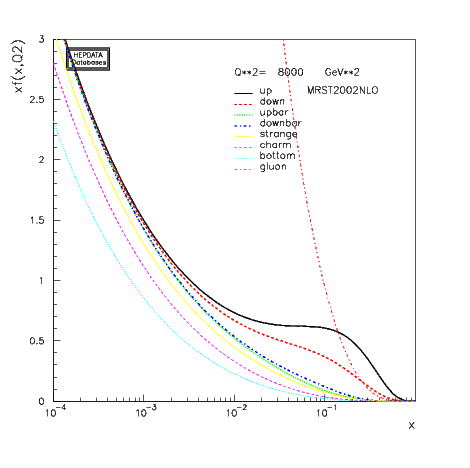
\includegraphics[scale=0.5]{THESISPLOTS/PDF_TEN.png}
%\captionof{figure}{Pdfs.}
%\label{fig:pdfs}
%\end{center}
%It is imperative to know the uncertainty in the measurement of PDFs as this is usually a source of uncertainty in a related experiment.
%%%%%%%%%%%%%%%%%%%%%%%%%%%%%%%%%%%%%%%%%%%%%%%%%%%%%%%%%%%%%%
%\newline
%The value of the strong coupling $\alpha_{S}$ which determines the strength of the strong interaction depends on the momentum transfer $Q^{2}$ as do the coupling constants of the $SU(2) \times U(1)_{Y}$ groups.
% For large $Q^{2}$, $\alpha_{S}$ approaches zero in a process in QCD referred  to as \textit{asymptotic freedom} and the quarks are nearly free while for small values of $Q^{2}$, $\alpha_{S}$ grows large and the quarks are tightly bound. This process is also referred to as \textit{confinement}.
%Quarks are always confined to hadronic bound states called baryons or mesons consisting of three quarks or a quark and anti-quark respectively.
%\newline
%The proton is the most stable baryon. It is made up of two up quarks and one down quark such that its electric charge is 1. These are called valence quarks. It turns out that from experiments, valence quarks are not the only quarks present in a proton. Infact it is best to describe the proton as made up of \textit{partons}. Partons are quarks and gluons. 
%Inside a proton, it is possible for a gluon to radiate or split up into a quark anti-quark pair. These kind of quarks are referred to as sea quarks. All partons in a proton carry the total momentum of the proton, however during proton-proton collision in a hadron accelerator, the partons are the actual colliding particles and not the protons so it is imperative to know the momentum fraction \textit{x} of an individual parton inside a proton. The momentum fraction of a parton is expressed as a \textit{Parton Distribution Functions}~(PDFs).
% very well when performing a search for physics beyond the SM as calculating scattering \textit{cross sections} which is an experimentally observable quantity describing the probability of a particular process happening highly depends on PDFs. In addition to this, due to the PDFs, the center of mass for proton-proton collision which in actual experiment is parton-parton collision is much reduced from $\sqrt{s} = 14$ \TeV as advertised in the LHC to $\sqrt{\hat{s}} \approx 2$ \TeV and this depends on the particular partons involved in the parton-parton interaction.
%\paragraph*{}
%Without the Higgs mechanism, all the particles described so far will be massless. But experiments observe massive particles, So how do we get these particles to have mass in the SM?
%This questions remains and important one in particle physics. However in the case of the SM, we obtain mass by "manually" breaking the gauge symmetries in the SM through the addition of mass terms into the SM Lagrangian. Thus the introduction of mass terms through the Higgs mechanism breaks the local gauge invariance in the theory which describes all the above interactions.

% This combination is expressed  as given in equation \ref{eq:SYM}.
%The symmetry groups describe the following parts of the SM interactions:
 %defines the strong nuclear interaction where quarks with color charge C are coupled to massless  eight( octet ) gluons in the frame work of QCD. The surprising phenomenon here is that unlike electromagnetic interactions ~(QED) where massless photons cannot interact with each other, these massless guons can interact with each since they carry color charge. There are three color charges.
%As previously mentioned, no free quark has been observed, rather, quarks exist in nature in the form of bound states called \textit{hadrons}. Hadrons can either be \textit{mesons}, which means, they are made up of a quark-antiquark pair like pions~(\Ppizero,\Ppipm) or \textit{baryons}, which means they are made up of 3 quarks like protons. Recent experiments have observe bound states consisting of $4$ quarks \cite{Quarks}, which remain consistent with the nature of  strong interactions between quarks in nuclei.

%%
 
%It is interesting to note that particles with spins, $s =\Big\{\mathbf{0}, \frac{1}{2}, 1\Big\}\hbar$, describe very precisely only $4.6$\% of the entire matter in the universe using the SM. 
%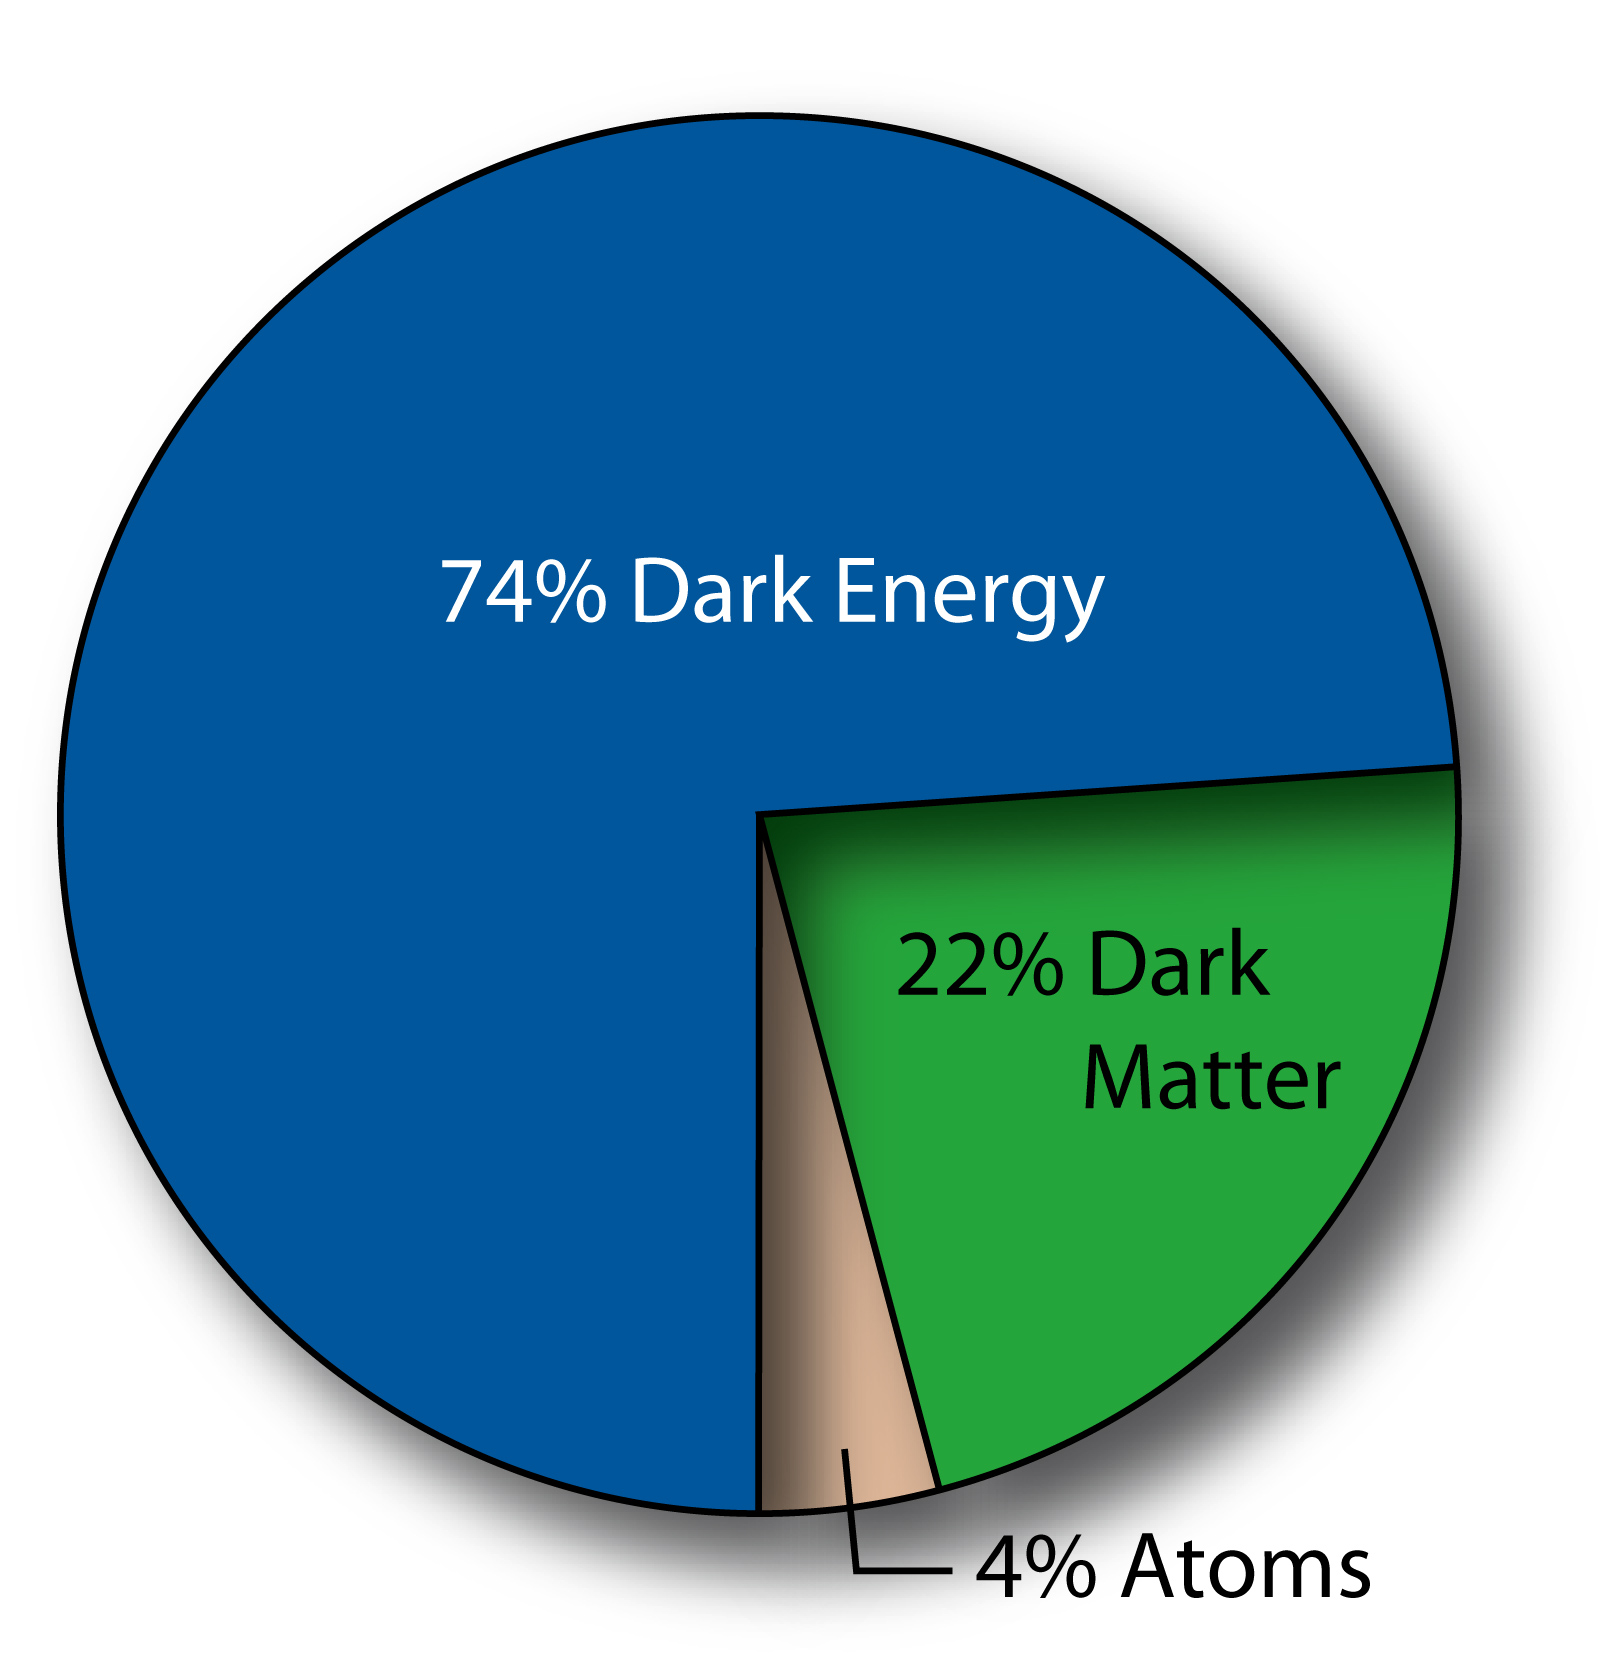
\includegraphics[height=1.7cm,width=0.25\paperwidth]{THESISPLOTS/UniversePie30.jpg}
%\end{frame}
%The above particles and their nature of interaction is described mathematically using the 
%The SM is a \textit{relativistic quantum field theory} in which particles are represented as \textit{quantum fields} and their dynamics and interaction with other particles can be expressed using a mathematical function called  the \textit{Lagrangian density}, $\mathcal{L}$. The Lagrangian density is invariant under certain transformations or symmetries and carries the description of the dynamics of fermions, bosons and their interactions with other bosons including the Higgs boson. Fermions and bosons get their mass through interacting with the Higgs boson in a process crucial to the SM known as  the \textit{Higgs Mechanism}.
%Our brief description of the SM, will be divided into the following sections:
%\begin{itemize}
%\item \textbf{\textit{Fermions}}: All of visible matter is described using fermion fields.
%\item \textbf{\textit{Interactions}}: Fermions interact either through electromagnetic, weak and strong interactions with vector bosons mediating  these interactions. An interaction is the realization of some generic symmetry and associated with this symmetry is a conserved quantity.
%\item \textbf{\textit{Spontaneous Symmetry Breaking or Higgs Mechanism}}: Fermions originally have no mass. They get their mass by interacting with the Higgs field through the \textit{Higgs mechanism}. New states of matter or fermions can be formed through mixing with other states of matter or fermions.
%\end{itemize}
%\begin{equation}
%INSERT HIGGS DOUBLET HERE 
%\end{equation}
%which is invariant uder the gauge symmetry group $SU(2)_{L} \times U(1)_{Y} $  and has its dynamics described by the Lagrangian density:
%\begin{equation}
% HIGGS DOUBLET LAGRANGIAN
%\end{equation}
% responsib is the Higgs doublet with spin-0 complex components.
%The parameter $\mu^{2} < 0 $ and the real parameter $\lambda > 0$ of the scalar Higgs potential(figure \ref{fig:Higgs}).
%is chosen such that the potential $V \rightarrow \infty $ as $\mathbf{\Phi} \rightarrow  0 $.
%It is easily seen from the previous equation that the minimum of the potential is not longer at $\mathbf{\Phi} = 0 $ but  lies at :
%With this choice of parameters settings, the potential V is itself $SU(2)_{L}$ symmetric but any other choice of ground state breaks $SU(2)_{L}$ symmetry. This is referred to as the \textit{Higgs-Brout-Englert mechanism} or \textit{Higgs mechanism} for simplicity.
%This choice of parameters of the potential V can be seen in figure below.
%\begin{equation}
%put higgs potential picture in here!
%\end{equation}
%One can then choose $\phi_{1} = \phi_{2}= \phi_{3} = 0$ and then parametrise the higgs doublet as small perturbations around the minimum as follows:
%\begin{equation}
%equation of higgs pertubations
%\end{equation}
%with $h(x), \eta_{i}(x)$ being 4 real scaler fields. Using the gauge freedom of $SU(2)_{L} \times U(1)_{Y}$ once can choose the \textit{unitarity gauge} where the kinetic terms for the fields $\eta_{i}(x)$ vanish and their with the requirement of local gauge invariance, $\eta_{i}(x)$ couple to the massless gauge bosons to be to become massive and the resulting Higgs doublet is expressed as:
%\begin{equation}
%Higgs doublet with imaginary parts removed
%\end{equation}
%With the imaginary parts removed and the  field $h(x)$ is identified as the physical real scalar Higgs field or Higgs boson.
%The ground state chosen so that the photon remains massless while the other gauge bosons including the real scalar Higgs field are massive with their masses given as:
%\begin{equation}
%Eqns of Gauge boson masses and Higgs mass
%\end{equation}
%The $Z^{0}$ mass $m_{Z}$ can also be expressed in terms of the $W^{\pm}$ mass $m_{W}$ and the Weinberg angle as:
%\begin{equation}
% Z mass to W mass equation
%\end{equation}
%Thus one can easily observe that all the effects of the W and Z bosons can be described in terms of the parameters $e$, $\theta_{w}$ and $\nu$ which can be expressed in term of Fermi constant all of which were experimentally known. Thus it is fine to say that the Higgs mechanism could predict the masses of W and Z gauge bosons which were experimentally found and measured in 1983 at LEP\cite{}.This discovery was one of the greatest triumphs of the SM.
%With the value of $\nu \approx 246$~GeV, we can then express the mass of the fermions in terms of the Yukawa coupling as ( from the Yukawa sector of the Lagrangian) :

%%%%%%%%%%%%%%%%%%%%%%%%%%%%%%%%%%%%%%%
%The SM predictions of the value of the Higgs boson's mass recommend additional contributions from \textit{quantum fluctuations}~(higher order or loop corrections) which are very large~(can as well be infinite). However, the observed experimentally measured value of the Higgs mass~($m_{H} \approx 125$~\GeV). This unobserved large corrections to the experimentally measured value requires some understanding. A possible explanation is that these various contributions cancel on average producing a net zero effect on the true Higgs mass such that the physically observed mass is as measured. If such cancellation is a true phenomenon in nature, then it is only logical to inquire the origin of this cancellations. Obviously this cannot be understood within the frame work of the SM. 

%Consequently, theories beyond the SM like \textit{supersymmetry} provide a natural understanding of how these various contributions cancel on average arriving at the physically observed and measured Higgs mass. To expand further, the mass of a particle can be expressed as 
%\begin{equation}
% m^{2}_{\mbox{physical}} = m^{2}_{\mbox{bare}} + \delta m^{2}_{1}
%\end{equation}

%where $m^{2}_{\mbox{physical}}$ is the physically measured mass of the Higgs boson,  $m^{2}_{\mbox{bare}}$ is the true  universe given mass of the particle which cannot be calculated or measured. $\delta m^{2}_{1}$ are corrections from quantum fluctuations to the true mass which can be calculated. Using the measured mass and the calculated  quantum corrections, one can obtain the true Higgs mass. These contributions from quantum fluctuations can arise from both bosons and fermions. Since the Higgs boson can interact~(by coupling) with every particle through interactions of the general form $\lambda_{f}H\bar{f}f$ for fermions and $\lambda_{S}|H|^{2}S^{2}$ for scalar or bosons;  with $\lambda_{f}$ and $\lambda_{S}$ representing the coupling constants which need not be equal. The Feynman diagrams in \ref{fig:Hmass} represents a few of such quantum fluctuations with both fermion and boson contributions computed as:
%Putting Figures side by side.

%%% GGM Stuff

% Thus the decay length, $c\tau$  for electromagnetic interaction, can be very different to that of weak and strong interactions. The decay length for strong interactions is the shortest because of the strong nature~(coupling constant $\approx 1$) of strong interaction. The weak and electromagnetic interactions have much smaller coupling constants thus often leads to longer decay length. There are some exceptions to this due to other factors playing a key role than only the strength of a given interaction such as the size of the available phase space and the difference in mass between the parent and the sum of the mass of the daughter particles.
%The table and graph below show the mass and decay length of SM particles and their interaction.
%\begin{equation}
% TABLE SHOWING SM particle decay rates and interactions involed as well as mass Vs decay length.
%\end{equation}
%In particle physics experiments it is very challenging to measure the  life time or decay length or a particle  by measuring the time it travels from where it was produced to where it decayed. Rather, the number of events present initially and that observed after a time period t is used to measure the lifetime of a particle. The decay rate ( or life time) of a particle is related to the number of particles observed though the equation:
 %\begin{equation}
% N(t) = N_{0}\exp\left(\frac{-t}{\tau}\right) = N_{0}\exp\left(\frac{-\Gamma t}{\hbar}\right) 
 %\end{equation}
%where \textit{N(t)} is the number of particles observed at an arbitrary time \textit{t} and $N_{0}$ is the number of particles observed at an initial time where it is assumed no particle has decayed yet usually at $ t = 0 $.
%A distribution of the observed number of particles( usually a Poisson distribution) can be plotted with time measured. The resulting distribution if fitted with a Poisson distribution faction and the parameter of the Poisson distribution function extracted  to give us the decay rate or life time of a particle.
%\newline
%Particles with large decay length or long life time are commonly referred to as \textit{Long-Live}~(LL) particles. Many models beyond the SM predict the existence of such particle. They are also understood to be prime candidates for particles making up DM.
%Before we dive into such models, it is necessary to understand in detail the decay of particles and factors which determine a particle's decay length as well as the kind of LL particles considered detectable in a multi-particle physics detector such as those at the Large Hadron Collider~(LHC) CERN pursued in this thesis.
%\paragraph*{}
%Particles described by the SM come in different types of long-lived.  First, we have the stable elementary (as we currently believe) such as the electron and neutrinos. Second, we have the meta-stable elementary such as the muon and finally the (very) long-lived composite particles such as the neutrons and protons. By referring to the different classes of particles according to their life time, we can asked the question, what properties of a particle makes it stable, meta-stable or long-lived?
%\newline
%There are three possible answers to this question:
%\begin {itemize}
%\item A particle could be the lightest state carrying a conserved quantum number and as such remain entirely stable e.g the electron and proton.
%\item The decay of a particle to another lighter particle could only be  made possible through some suppressed or effective coupling and as a result ends up being meta-stable e.g the muon
%\item If the mass of a particle is relatively close in quantity to the particle it is decaying into such that their difference in mass is quite small, the decay will be eventually suppressed. This goes by the name lack of phase space for decay e.g decay of neutron ($ n \rightarrow p + e^{-} + \bar{\nu}_{e} $). In this scenario the difference in mass between the neutron (n) and the proton (p) is $\approx 1.293$ MeV and as a result determines the type of associated particle produced in this decay as observed.
%\end{itemize}

%long-lived particles in this thesis, we cover mostly \textit{massive neutral meta-stable} particles  referred here as \textsf{Neutral Massive Long-Lived Particles}~(NMLLP). These are either elementary or composite neutral particles with life-time within the detectable range of a collider detector i.e few nanoseconds. In general, 
%A rather more descriptive name would be Neutral Massive Meta-Stable Particles(NMMP) since these particles are not very long-lived in the real sense but might decay into other elementary particles which for all practical purposes can be observable at collider detectors.
%\newline
%We have restricted ourselves to electromagnetic (local U(1) gauge symmetry) neutral particles as their charge counterparts can be studied using conventional magnetic spectrometer and ionization methods as shown in this studies for Heavy Stable Charge Particles (HSCP).
%%%%%%%%%##############################################################################################
%These are Soft breaking mean the SUSY breaking terms in the SUSY potential~(eqn \ref{eq:SUSYEQ}) consists of only masses and terms whose couplings have positive mass dimension. This ensures the existence of sparticles with masses around a few \TeV where they can possibly be produced at current particle colliders such as the large hadron collider~(LHC).
%\newline
%RPC models are those discussed in this thesis as our search is motivated towards the search for neutral stable particles as possible candidates particles for dark matter~(DM).
%\paragraph*{•}
%If SUSY is a theory which describes nature, then its prediction of components within the same supermultiplets with the same mass, i.e $m_{B}= m_{F}$ is not realistic, since  experiments are yet to find a selectron~(SUSY partner of electron) with a mass of 0.512\MeV for example. Therefore, SUSY must be realized through a spontaneously broken way. Spontaneous Supersymmetry Breaking~(SSB) means the lowest energy state or vacuum expectation value of a scalar field~(or auxiliary field as is the case with SUSY) must be non-zero. The type of breaking  determines the phenomenology of any given model. We focus on models with gauge interactions responsible for communicating SUSY breaking from a higher energy level to our observable collider experiments energy levels. Gauge Mediated SUSY breaking models~(GMBS) can be Pure, General or minimal Gauge Mediation~(GGM)depending on the model parameters.
%The presence of the hadron collider in CERN, has encouraged the development of SUSY models whose predictions are about a few \TeV for the mass range of some of these SUSY particles and also the energy scale which the most powerful particle colliders can probe for new particles. These kind of models are called Soft SUSY Breaking models. We would focus on such models in particular the 
%\subsection{Soft Supersymmetry Breaking}
%Soft SUSY breaking is such that the spontaneous breaking must be caused by couplings with positive mass dimension and not dimensionless coupling. This allows for the alredy observed hierarchy between the Electro-Weak energy scale of $\approx 100$\GeV and the reduced Planck energy scale $ \approx 10^{18}$\GeV .
%The Lagrangian for soft SUSY breaking terms  can be written as thus:
%\begin{align}
%\mathcal{L}^{\mbox{mssm}}_{\mbox{soft}} &= -\frac{1}{2}\left( M_{3}\tilde{g}\tilde{g} + M_{2}\tilde{W}\tilde{W} + M_{1}\tilde{B}\tilde{B}\right) + c.c + \cdots \\
%& -\left(a_{u}\tilde{\bar{u}}\tilde{Q}H_{u} - a_{d}\tilde{\bar{d}}\tilde{Q}H_{d} - a_{e}\tilde{\bar{e}}\tilde{L}H_{d} + c.c \right)
%\end{align}
%&- m^{2}_{H_{u}}H^{*}_{u}H_{u} - m^{2}_{H_{d}}H^{*}_{d}H_{d} - \left( bH_{u}H_{d} + c.c. \right) \\
%&- m^{2}_{Q}\tilde{Q}^{+}\tilde{Q} - m^{2}_{L}\tilde{L}^{+}\tilde{L} - m^{2}_{\bar{u}}\tilde{\bar{u}}^{+}\tilde{u}-m^{2}_{\bar{d}}\tilde{\bar{d}}^{+}\tilde{d} -m^{2}_{\bar{e}}\tilde{\bar{e}}^{+}\tilde{e}\\
%where $M_{1}$, $M_{2}$ and $M_{3}$ are the superpartners of the gauge bosons of the SM symmetry group. They are referred to as the \textit{Bino}~($\tilde{B}$), \textit{Wino}~($\tilde{W}$) and \textit{gluinos}~(8 gluinos because there are 8 gluons in the SM). I have intentionally omitted  scalar mass terms in this Lagrangian, if interested in the rest of the terms see \cite{SM}.
%\paragraph{General Model}
%\paragraph*{•}
%Constructing a SUSY model requires that the model has gauge group describing the nature of particle interaction, a superpotential, and since the SUSY prediction of equal masses of boson and fermions is not observable, one must provide explicitly the method for spontaneously breaking supersymmetry. We have in the MSSM scenario seen the gauge groups to be exactly those of the SM, the superpontential with soft terms, however, we are yet to understand how supersymmetry is broken. SUSY breaking means that we find the lowest energy state for which the vacuum expectation values of the  SUSY generators $\mathrm{Q}_{\alpha} \ket 0 \neq 0$ or $\bar{\mathrm{Q}}_{\alpha}\ket 0 \neq 0$. Since one can always express the Hamiltonian of the system, $\mathrm{H}$ in terms of the SUSY generators, SUSY breaking can also be equally expressed as $\mathrm{H}\ket 0 \neq 0$. Neglecting spacetime-dependent effects and condensates, SUSY breaking is equivallently expressed as $\mathrm{V}\ket 0 \neq 0$, where $\mathrm{V}$ is the standard superpontential expressed in terms of the $\mathrm{F}$ and $\mathrm{D}$ terms. Thus, spontaneously breaking SUSY is equivalent to finding superpotentials for which neither $\mathrm{F}$ nor $\mathrm{D}$ terms simultaneously vanish in the lowest energy state. Suoerpotentials with non vanishing $\mathrm{F}$ terms are called  \textit{O'Raifeartaigh} or $\mathrm{F}$-term SUSY breaking models while those with nonvanishing $\mathrm{D}$ terms are called \textit{Fayet-Illiopoulus} or $\mathrm{D}$-term SUSY breaking models. Since in GMSB models, it is the $\mathrm{F}$ term which has a non-vanishing lowest energy state expectation value or vacuum expectation, this thesis only considers  \textit{O'Raifeartaigh} SUSY breaking models.
%\newline
%In GMSB models, this superpotential is termed the \textit{Hidden Sector}~(hidden because it couples only indirectly and very weakly to our "observable sector" of SM particles and their superpartners) and it is its dynamics which spontaneously breaks supersymmetry. The nature of this breaking is not relevant for phenomenology but rather the "\textit{mediators}" which communicate the effects of this breaking to the superpartners of the SM particles. Therefore, these mediators or agents must couple to this "Hidden Sector" as well as the "observable sector".
%This \textit{Messenger fields} in GMSB, have the usual SM gauge interactions  and through loops couple with the SM superpartners. As a result MSSM particles~(gauginos and sfermions) obtain SUSY breaking masses referred to as \textit{soft terms} through loop level interactions. This procedure allows for the observed mass and energy scale hierarchy is maintained. The mass of these messenger fields, $\displaystyle{\mathrm{M}_{\mbox{mess}}}$, along with $\left\langle\mathrm{F}\right\rangle$  defines the energy scale at which supersymmetry breaking is felt at the MSSM energy scale. If $\displaystyle{\mathrm{M}_{mess} \ll \mathrm{M}_{\mbox{Planck}}}$, $\mathrm{M}_{\mbox{Planck}} \approx 10^{19}$\GeV, then supersymmetry breaking occurs at a much lower energy scale instead at the Planck energy scale where gravitational interactions become very significant and the effects of the breaking is first felt by these Messenger fields and later communicated to the observable sector through SM gauge interactions.
%In terms of energy scales, the picture is such that spontaneous supersymmetry breaking occurs at an energy scale, $\left\langle\mathrm{F}\right\rangle$ which we denote as $\mathbf{F}$, for simplicity. This energy scale defines the mass, as seen in equation \ref{eq:GMass}, of the \textit{gravitino} which is the supersymmetric partner of gravity mediating particle, the \textit{graviton}. The gravitino has the same quantum number as the Nambu-Goldstone particle, the massless neutral Weyl fermion, the \textit{goldstino}, originating from supersymmetry breaking. 
%\begin{equation}{\label{eq:GMass}}
% m_{3/2} = C_{grav}\cdot\frac{\mathbf{F_{s}}}{{\sqrt{3}\mathrm{M}_{Pl}}}
%\end{equation}
%where $\displaystyle{\mathrm{M}_{Pl} = 1.3 \times 10^{19}}$~GeV.

%In GMSB models, the energy scale for which supersymmetry breaking is transmitted to the Hidden sector, $\mathbf{F}_{s}$ might not be the same as the original or fundamental sypersymmetry breaking energy scale, $\mathbf{F}$. If $\displaystyle{\mathbf{F}_{s} < \mathbf{F}}$ then the interaction between the hidden sector and the fundamental SUSY breaking is weak interaction and if $\displaystyle{\mathbf{F}_{s} \approx \mathbf{F}}$ and the interaction is strong.  It is necessary that this interaction is weak, as in this case GMSB models do not surfer from flavor violating interactions which are not observed in nature.
%The induced SUSY breaking scale in the hidden sector ${\mathrm{F}}_{S}$ and the mass of the messenger particles  defines the mass spectrum of the particles in the MSSM sector.
%The consequences of this is that one would no longer expect the mass of the gravitino $m_{3/2}$ to be given as in equation \ref{eq:GMass} but rather suppressed by $\mathrm{M}_{\mbox{mess}}/\mathrm{M}_{Pl}$ in GMSB models. In this mass spectrum scenario, the gravitino mass can be varied to a very small value only bounded by cosmological results, thus making it the lightest supersymmetric particle~(LSP). Spanning the gravitino mass is expressed as a fundamental parameter in GMSB modles, $C_{grav}$ which directly determines the lifetime of the next-to-lightest supersymmetry sparticle  decaying to the gravitino. We will see more of this ahead. Thus the parameters $\mathbf{F}_{s}$ and  $\mathrm{M}_{\mbox{mess}}$, determines the masses of the gauginos and sfermions of the MSSB in GMSB models.
%\newline
%A minimal GMSB model is one where the messenger sector consists of chiral supermultiplets of leptons and quark with the same quantum numbers $SU(3)_{C}\times SU(2)_{L}\times U(1)_{Y}$ as the SM gauge groups. That is, the messenger fields belong to some $SU(5)$ gauge group. The representations of these messengers fields are given in equation \ref{eq:MESS}.
%\begin{align}{\label{eq:MESS}}
%\tilde{\ell} \sim (1,2,1) \quad \tilde{\ell^{\prime}} \sim (1, 2^{\star}, -1) \\
%\tilde{q} \sim (3,1,-\frac{2}{3}) \quad \tilde{q}^{\prime} \sim (3^{\star}, 1, \frac{2}{3} )
%\end{align}
%These messenger fields, via a superpotential as in equation \ref{eq:WMESS} of a gauge singlet chiral supermultiplet $\mathrm{S}$, couple with an $\mathrm{F}$-term as in the O'Raifeartaigh model \cite{SM}. 
%\begin{equation}{\label{eq:WMESS}}
%W_{\mbox{mess}} = \lambda_{\ell}\mathrm{S}\tilde{q}\tilde{q}^{\prime} + \lambda_{q}\mathrm{S}\tilde{\ell}\tilde{\ell^{\prime}}
%\end{equation}
%We thus obtain SUSY breaking by allowing vacuum expectation values~(VEV) for both $\mathrm{S}$ and its auxiliary component $\mathrm{F}$ term as $\left\langle \mathrm{S} \right\rangle$ and $\left\langle \mathrm{F}_{s} \right\rangle = \mathbf{F}_{s}$, where the $\mathbf{F}_{s}$ does not have to coincided with $\mathbf{F}$ as mentioned earlier. The parameter representing this non equivalence,$C_{grav}$ is defined as shown in equation \ref{eq:CGRAV}. It is one of the fundamental parameters in GMSB models responsible for the lifetime of NLSP particle.
%\begin{equation}{\label{eq:CGRAV}}
%\mathbf{F} = C_{grav}\cdot\mathbf{F}_{s}
%\end{equation}
%This equation indicates that the non-zero VEV for the $\mathrm{F}$ term is responsible for fundamental SUSY breaking which is transferred to the messenger particles through radiative interactions as $C_{grav}$ is a dimensionless parameter.
%Leptons and fermions masses(\ref{eq:MMass}) of the messenger particles together with their scalar superpartners are obtained from diagonalizing the mass matrix.
%\begin{align}{\label{eq:MMass}}
%m^{2}_{\tilde{\ell}\tilde{\ell^{\prime}}} &= |\lambda_{\ell}\left\langle \mathrm{S} \right\rangle|^{2}, \quad \quad  m^{2}_{\tilde{\ell}_{\mbox{scalars}}} = |\lambda_{\ell}\left\langle \mathrm{S} \right\rangle|^{2} \pm |\lambda_{\ell}\left\langle \mathrm{F_{s}} \right\rangle |
%\\
%m^{2}_{\tilde{q}\tilde{q^{\prime}}} &= |\lambda_{q}\left\langle \mathrm{S} \right\rangle|^{2}, \quad \quad  m^{2}_{\tilde{q}_{\mbox{scalars}}} = |\lambda_{q}\left\langle \mathrm{S} \right\rangle|^{2} \pm |\lambda_{q}\left\langle \mathrm{F_{s}} \right\rangle |
%\end{align}
%By observing equation \ref{eq:MMass}, a general energy scale, $\mathbf{M}_{\mbox{mess}}$, for messenger particle's masses which is also an additional fundamental parameter in GMSB models can be defined as shown in equation \ref{eq:Mmess}.
%\begin{equation}{\label{eq:Mmess}}
%\mathbf{M}_{\mbox{mess}} = (\lambda_{q},\lambda_{\ell}) \left\langle \mathrm{S} \right\rangle 
%\end{equation}

%A common assumption in GMSB models according to~\cite{GMSB, SUSYBOOK} is that $\lambda_{q} \simeq \lambda_{\ell} \simeq \lambda $ and so $\mathbf{M}_{\mbox{mess}} = \lambda \left\langle \mathrm{S} \right\rangle$. However, in  Pure gauge mediated SUSY breaking models~(PGGM), $\lambda_{q} \neq \lambda_{\ell}$ \cite{PGGM}.
%In the MSSM sector, gauginos and scalars obtained their mass through one-loop and two-loop level interactions respectively given according to equation \ref{eq:MSSMMasses}.
%\begin{align}{\label{eq:MSSMMasses}}
%\mathbf{M}_{a} &= \frac{\alpha_{a}}{4\pi}\mathrm{N_{5}}\mathbf{\Lambda} \\ 
%\mathbf{m}^{2}_{\phi_{i}} &= 2\mathbf{\Lambda}^{2}\mathrm{N_{5}}\sum_{a=1}^{3}C_{a}(i) ( \frac{\alpha_{a}}{4\pi})^{2}
%\end{align}
%where $C_{a}(i)$ are constants of $\mathsf{O}(1)$, $\alpha_{a}$ are coupling constants and 
%\begin{equation}{\label{eq:Lambda}}
%\mathbf{\Lambda} = \frac{\mathbf{F}_{s}}{\lambda \left\langle \mathrm{S} \right\rangle } = \frac{\mathbf{F}_{s}}{\mathbf{M}_{\mbox{mess}}}
%\end{equation} 
%$\mathrm{N_{5}}$ is an additional parameter in GMSB models, specifying the number of messenger vector-like supermultiplets transforming under $SU(5)$. A motivation for $SU(5)$ is for the unification of gauge couplings at the GUT energy scale($M_{GUT} \approx 10^{16}$~GeV which is one of the major predictions of supersymmetry in unifying fundamental forces.
%$\mathrm{N_{5}}$ is chosen to be not very large so as to avoid gauge couplings diverging before GUT scale. In the minimal GMSB models such as the SPS8 benchmark working point model $\mathrm{N_{5}} = 1$.
%A simple diagrams for these corrections can be seen in figure \ref{fig:figMass}.
%\begin{figure}[ht]{\label{figMass}
%\begin{minipage}[b]{0.45\linewidth}
%\centering
%\includegraphics[height=7cm, width=\textwidth]{OneLoop_Gaugino_Mass.png}
%\caption{$c\tau_{\chi^{0}_{1}}$[mm]}
%\label{fig:1-loop level contributions from messenger particles giving rise to MSSM gaugino mass. The dashed(single) lines are messenger scalars(fermions).}
%\end{minipage}
%\hspace{0.5cm}
%\begin{minipage}[b]{0.45\linewidth}
%\centering
%\includegraphics[height=7cm,width=\textwidth]{TwoLoop_MSSM_Scalar_Masses.png}
%\caption{$Boost_{\chi^{0}_{1}}$ }
%\label{fig:2-loop level contributions from messenger particles giving rise to MSSM gaugino mass. The dashed(single) lines are messenger scalars(fermions) while the wavy lines are SM gauge bosons}
%\end{minipage}
%\end{figure}
%On the other hand in PGGM models~(\cite{PGGM}), gauge and scalar particles have separate mass definitions~(eqn:\ref{eq:MPGGM}) since $\lambda_{q} \neq \lambda_{\ell}$.
%\begin{align}{\label{eq:MPGGM}}
%\mathbf{\Lambda}_{G} &= \frac{\mathrm{F}_{s}}{\lambda_{q} \left\langle \mathrm{S} \right\rangle } \\
%\mathbf{\Lambda}_{S} &= \frac{\mathrm{F}_{s}}{\lambda_{\ell} \left\langle \mathrm{S} \right\rangle } 
%\end{align}
%$\mathbf{\Lambda}$ is the energy scale defining SUSY breaking at the MSSM level. It is known as the \textit{effective supersymmetry breaking scale} and determines the mass spectrum of gauginos and scalars in the MSSM.
%$\mathbf{\Lambda}$ as defined in equation \ref{eq:Lambda} is considered to be a model parameter in GMSB models especially in minimal GMSB modles like the SPS8 bench mark model.
%It is important to not that GGM models, \cite{GGM, GGM1, GGM2,MDINE1,MDINE2}, the mass of the gauginos $\mathbf{M}_{a}, a = 1,2,3$ defines the parameter space for these models.
%Using equation \ref{eq:CGRAV}, the fundamental SUSY breaking scale $\mathbf{F}$ can be redefined in terms of the effective SUSY breaking scale $\mathbf{\Lambda}$  and the Messenger particle mass scale $\mathbf{M}_{\mbox{mess}}$:
%\begin{align}{\label{eq:scale}}
%\mathbf{F} = C_{grav}\cdot \mathbf{\Lambda}\cdot\mathbf{M}_{\mbox{mess}} 
%\end{align}
%and from equation \ref{eq:GMass}, the gravitino mass is re-written shown in equation \ref{eq:GMass2}
%\begin{align}{\label{eq:GMass2}}
%m_{\tilde{G}} & = C_{grav}\cdot \frac{\mathbf{\Lambda}\mathbf{M}_{\mbox{mess}}}{\sqrt{3}\mathrm{M}_{pl}}
%\end{align}
%In summary, the parameters $\mathbf{\Lambda}$, $\mathrm{N_{5}}$, and  $C_{grav}$  determines the phenomenology of GMSB models.The gravitino can become very light with its mass bounded only by cosmological observations and as such is identified as  the least stable supersymmetry particle~(LSP). By changing the value of $C_{grav}$, which is equivalent to scaling the induced supersymmetry breaking energy scale, allowing for weak interactions between the hidden sector and the messenger particles, the mass of the gravitino, $m_{\tilde{G}}$, is changed. This influences the decay rate and lifetime of the next-to-lightest supersymmetry particle~(NLSP) decaying to the gravitino which can vary from being an instantaneous or prompt decay to being a long-lived particle decay.

%% Decay width stuff
%Particles which live long enough to travel distanced comparable to the detector size(of the order of a few minutes) are equally referred to as \textit{long-live} particles.  
%Almost all particles disintegrate or \textit{decay}, most very rapidly. Collectively particles which disintegrate are said to be unstable while the few which do not are said to be stable. Those which take a long time to disintegrate are termed meta-stable or "\textit{long-lived}" particles. The length of the decay time and context will tell whether a particle is meta-stable or long-lived. The stability of a given particle is measured with respect to the age of the universe~(13.7 billion years). The only understood stable particles in nature are the \textsf{electron}(and \textsf{anti-electron})~($e$), \textsf{up}~($u$) and \textsf{down}~($d$) quarks and their anti-quarks, the \textit{photon}~($\gamma$), the lightest \text{neutrino}~($\nu_{e}$) and the \textit{graviton}. 
%Particles decay by transforming from one type of particle or generation unto another either through interactions, radiation or oscillation.  This decay, in analogous to our everyday experience depends on the their interaction strength with possible particles they can decay into. For example, strongly interacting particles will decay almost immediately while weakly interacting particles will naturally take some time. However, this is not the whole story, as quantum effects will also determine the particles nature of decay.
%which is understood to be about 13.7 billion years old. 
%Meta-stable particles which are composite~(bound states of elementary particles), are more unstable and easily decay into particles with smaller mass. An example of a meta-stable particle is the \textit{neutron}~(\textsf{$udd$}) which on its own, outside the atomic nucleus can remain stable for about 15 or so minutes. While, neutrons living inside some atomic neuclei can live for a period of time comparable to the age of the universe. Another meta-stable particle like the proton~(\textsf{$uud$}) seem very stable but can possibly decay after a very long period of time. It is speculated that the proton can remain stable for up to a period of about $10^{33}$ years. Atomic nuclei can also be considered as meta-stable living for about a tiny fraction of a second. Thus for all practical purposes, the proton is considered a stable particle while the neutron is considered a \textit{long-lived} particle.  It is believed that if \textit{dark matter} is made of particles then those particles  must be very, very, very long-lived with time also comparable  to or beyond  the age of the universe.
%Particle disintegration is understood as the interaction between a given particle and its daughter particle(s). This interaction could be electromagnetic, weak, strong, any pair or maybe all three types of interactions. 
%The stability of a particle is determined by the properties of the particle combined with  conservation laws of a quantum number or conserved quantity like energy, spin, momentum, angular momentum and charge. Other factors may also play an important role such as phase space~(availability of lighter particles to decay into), violation of some fundamental property like \textit{strangeness} or the mediating particle usually a boson being very massive compared to the momentum transfer between the parent and the daughter particle. These laws combined with particle's properties leads to a set of rules which are (almost) entirely determine whether a particle can decay or not or at most decay very rarely.  
%These set of rules can be summarized as follows:
%\begin{itemize}
%\item All particles must and should decay to two or more particles.
%\item The mass of the decaying~(parent) particle must exceed the sum of the mass  of the particles produced~(daughter particles) in its decay.
%\item There must be charge conservation i.e, the total electric charge of the parent particle must equal or match the total electric charge of the daughter particles.
%\item The total number of fermions or spin-1/2 particle before and after the decay must change only by an \textit{even} number.
%\item The total number of quarks minus the total number of anti-quarks must not change in any decay.
%\item The nature of of interaction and degree of phase space available must all be satisfied in order for any decay to take place.
%\end{itemize}

%This probability depends on the distribution of type of incoming particles inside the colliding protons with enough proton energy fraction to create a supersymmetric particle. Since the mass of the supersymmetric particle being create depends on the available center of mass energy of the colliding partons. In a hadron collider like the LHC, gluons are the one of these partons with the highest probability of proton energy fraction distribution. Sea quarks such as up and down quarks which make up the proton as well as valence quark which can exist inside the proton provide their energy fraction is large enough can also collide to create SUSY particles. The figure \eqref{PDFs} show the parton distribution function against its energy fraction on the horizontal axis within a proton. The probability of creating a SUSY particle depends on the momentum transfer $Q$ of these partons.

%% Stuff
%Since mass of SUSY particles like gluino, squarks and also neutralino is kept fixed by the SUSY effective breaking scale $\mathbf{\Lambda}$ as shown in equations \ref{eq:MSSMMasses}, the neutralino $\pt$ will depend o the number of associated quarks observed as \textit{jets} produced during the gluino or squark decay. Gluino or squark decays with very low jet multiplicity will lead to the production of large $\pt$ neutralinos which eventually leads to more boost factor while high jet multiplicity will lead to low $\pt$ neutralinos and hence low boost or $\beta$ factor. It is important to note that in either case, this depends also on the measured $\pt$ of the jets whether is low or high jet multiplicity cases. It is also worth mentioning that the photon produced from neutralino decay can also be arrived with large delayed time in situations where the photon arrival path to the detector is not a direct straight path but rather deviated as a result of a highly boosted neutralino produced from gluino or squark decay.

%In addition to the boost factor, the inherent proper decay length, $c\tau$,  will also determine the extend to which a long-lived neutralino is detectable at a particle detector. Neutralino with very long lifetime, $c\tau$, beyond the detectable length of the particle detector will obviously travel out of the detector before decay and as a result are often not detectable while neutralinos with very short lifetime may also be undetectable  as their decay length travel is not enough to be able to separate them for background events in a detector environment like the LHC unless other methods are employed like using its impact parameter distance travelled. However, this is only applicable in scenarios where the neutralino decays into a charged particle with tracks in the detector such that its decay production vertex can be used to correctly calculate and extracts the neutralino impact parameter or in other sophisticated detectors which the direction of the particle from neutralino decay is accessible. This the is case with ATLAS particle detector and not so with CMS detector.
%With $C_{grav}$, one could  one could change the decay length of the NLSP such that its decay occurs within the volume of the detector such that the resulting photon is delayed. This gives a unique signature for discovering SUSY in hadron colliders as photons produced from SM interactions are prompt
%\begin{equation}\label{DRate}
%c\tau_{NLSP} = 9.9 \times 10^{-8}\frac{1}{k_{1\gamma}}\left(\frac{m_{NLSP}}{100 GeV}\right)^{-5}\left(\frac{\sqrt{\mathrm{F}}}{10TeV}\right)^{4}
%\end{equation}

%%%%%%%%%%%%%%%%%%%%%%%%%%%%%%%%%%%%%%
%\subsection{Why is the search for neutral long-lived particles important?}
%\paragraph*{}
% Finding answers to fundamental questions such as the following: What is the origin of neutrino masses, Why are there only 3 types of leptons and quarks? Where do all the parameters in SM come from? Other big questions include: What is Dark Matter ~(DM)? is DM made of particles? Can one detect these particles? Why is there so much asymmetry between matter and anti-matter in our universe? Is there some energy scale or early epoch in the evolution of the universe where all the fundamental forces behaved as a unique kind of force. Do baryons such as the proton exist forever? What is the lifetime of the proton? What is Dark Energy~(DE)? Is the Universe expanding indefinitely? Are there other Universes? 
% provide added impetus to search for particles BSM. We believe that the discovery of a long-live particle which are not known to exist within the current SM will provide unique access to understanding physics BSM and making measurements which can provide answers to most of the above questions.
%\newline{}
%These questions have been addressed in two major fronts: Theoretically which involves lots of model building and Experimentally which can be divided into Observational as well as Collider Experiments. Most of these experiments involves the search for w new physics phenomenon. In this Thesis, we have decided to address some of these questions by searching for New Physics phenomenon or New Particles ~(NP) in a Hadron Collider experiment. 
%As a consequence, there are many searches for New Particles or New Physics~(NP) 
%Searching for LL neutral particles decaying to photon using timing gives us a unique advantage compared to other experiments as we expect very limited background process contribution from SM. Most of our background will be detector originated contributions
%Infact, we are searching for some NP which have been predicted to exist in nature by many Theoretical extensions of the SM collectively referred to as Beyond the Standard Model~(BSM). We will describe one of such models in the next section below.
%We are interested in searching for neutral NP through their lifetime. 
%Infact, our search using lifetime gives us a wide range of search techniques  depending on the lifetime of the LL particle ranging from quantitative measurements to statistics. The figure below  shows the wide variety of techniques which can be used to search for LL particles in general.
%\begin{equation}
%\mbox{ADD figure of techniques for Searches using LL}
%\end{equation}
%\begin{figure}
%\centering
%\includegraphics[scale=0.5]{}
%\caption{Different techniques to Search for LL particles.}
%\end{figure}
%Using equations \eqref{ctau}, precise measurement of fundamental parameters in SUSY or new physics can be archived.
%Another advantage is that, the our search for neutral particles  is unique in that a lot of previous searches been performed for charged particles but very limited for neutral LL particles since DM is speculated to be made of stable neutral particle(s) with long lifetime, we might as well go for DM. 
%We also use lifetime because no particle with lifetime $\gtrsim10^{-7}$~s and mass $\gtrsim 1.5$~GeV has been found and obviously because our detector has a very good timing resolution as can be seen in the section of the CMS detector in this thesis.
%\newline{}
%There have been previous attempts to search for quasi-stable neutral massive particles but all the search results show no evidence for neutral particles with long lifetime.  
%or neutral particles in general or neutral hadrons in particular 
%The challenge with such an experiment is that neutral particles cannot be studied using conventional magnetic spectrometer as they are not affected by magnetic field because they are charge~(local 
%U(1) gauge symmetry) neutral.
%Nevertheless, there are countless theoretical as well as observational reasons why studying these particles using novel experimental techniques is very important in the field of particle physics. 
%Some of these reasons will emerge naturally as we see in the subsequent sections below.
%We will attempt to give our humble lists of reasons in the following
%sections why we believe it is fundamental to study these particles.
%\subsubsection{Theory Motivation.}
%Physics BSM can be summarized to answering three major theoretical questions:  Is there a reliable explanation  
%behind the ordering in mass of SM particles as observed? This is the Hierarchy problem.
%Is there a single theory which can provide a derivation for all the 
%numerous parameters (19) in the SM and also unify all the fundamental forces of nature? Grand Unified Theories (GUT). 
%What is DM and Dark Energy (DE)?
%(DE is the stuff that is responsible for the accelerated expansion of our universe).
%And finally being a particle physicist it is only natural to ask if DM is made up of particles and if yes,
%Can one construct a model which can consistently describe DM as is already the case with visible matter in SM?
%\newline
%Most of the efforts in the last decades in theoretical particle physics has been to find answers to the above questions.
%\subsubsection{Experiment and Observation Motivation }
%As early as 1956 Reines and Cowan\cite{Neutrino} observed that when a neutron decays into a proton and an electron, an elusive particle called neutrino is also produced. The observation of neutrinos was later incorporated into the SM. In the formulation of the SM, the neutrinos are considered massless.
%However, recent results from experiments \cite{NeutrinoMix} have shown that neutrinos of different flavours can oscillate or mix into one another. The only way they can do this is if they have a tiny but finite mass. Recent experiments measuring the different neutrino flavours and their mass difference point towards the existence of a much larger theory that can incorporate the existence of neutrino masses and the observed phenomenon of neutrino mixing in which the SM is embedded in it   and can be understood as a low energy version of a much broader and deeper theory.
%\paragraph*{}
%Galactic and supernovae observations using the Hubble and a host of other telescope as well as results from Baryonic Acoustic Oscillation~(BAO) and WMAP reveal unique matter content of our universe. In addition to these cosmological observations including galaxy profiles,cluster formation, large scale structure formation and Cosmic Microwave background~(CMB) power spectrum can be somehow explained by DM \cite{WMAP}. These observation reveals about 25\% of our universe is made of DM with the current DM relic density is measured to be  %${\POmega}_{DM}h^{2} = {0.105} ^{\p 0.021}_{\m 0.030}$
%However, the question of "What is DM?" remains a very interesting one to both the particle physics astronomy society.
%Understanding DM and the rest of our universe will be crucial for future developments in high energy physics from both theory and experimental fronts.  
%A possible property of DM is that they must be made of up long lived neutral particles. There are candidate particles from SUSY which have these properties. A few of these include lightest neutralino~(\PSneutralinoOne) and gravitino~($\tilde{G}$). From the GMSB point of view, because gravitinos are stable, neutral and very weakly interacting; they are seen as good candidates for the particles which make up DM. 
%\subsubsection{Current Experimental Limits}
%Past Experiments seems to indicate that the remaining un %searched phase space for possible existence of SUSY particles %in shrinking.
%%%%%%%%%%%%%%%%%%%%%%%%%%%%%%%%%%%%%%%%%%%%
%%%%%%%%%%%%%%%%%%%%%%%%%%%%%%%%%%%%%%%%%
%\subsection{Physics}
%\paragraph*{}
% The SM of particle physics in all its glory is the most precise and well developed model describing and providing our understanding of how energy, space and time interact with each other. We will begin by describing the current status of the SM highlighting areas where there could be need for further development in the format of questions.

%%% Beyond SM
%$\Lambda$ is some \textit{cut-off} energy scale where a another kind of physics interaction like gravity at a much higher energy scale is needed to regulate the low energy behavior of the SM. $\Lambda$ could be the reduced Planck scale(~ $10^{18}$~\GeV).  A quick observation from this calculations is that; first, corrections to the higgs bare mass, $m^{2}_{\mbox{bare}}$ are not proportional to the Higgs mass.
%( in other cases like as is the case with other SM particles like the electron\cite{}.
%Second, these corrections are of the order of $\approx 10^{36}~\GeV^{2}$  bringing positive and negative contributions from fermions or scalar bosons respectively.
%Even with these corrections to the true Higgs mass, the measured~(physical) Higgs mass squared, $m^{2}_{H,\mbox{physical}}$, is of the order $\approx 10^{4}~\GeV^{2}$.
%Since the true Higgs mass, $m^{2}_{H,\mbox{bare}}$, is never measured or known, an agreement between these quantum fluctuation contributions and physical Higgs mass is realized  if only the true Higgs mass, $m^{2}_{H,\mbox{bare}}$,  is \textit{fine-tuned} with a precision of about 1 in $10^{17}$. This enormous fine-tuning is considered a fundamental issue of not enough understanding of the Higgs mechanism of the SM and is considered \textit{unnatural}. 
%The fact that, among the numerous SM predictions, no other scalar particle except the possible Higgs boson candidate has been observed so far, further makes such a fine-tuning difficult to understood. 
%On the other hand, in suppersymmetry, the fermion one loop quantum correction which comes with an opposite sign to the scalar quantum fluctuation corrections and $\lambda_{f} = \lambda_{S}$ ,there is a complete  cancellation and this discrepancy of the unobserved effects of these quantum fluctuations to the $m^{2}_{H,\mbox{bare}}$ in the $m^{2}_{H,\mbox{physical}}$ is understood. 
% Another interpretation of this issue is through the question of why there is so much difference in energy scale between the electroweak scale \textit{O}(100~\GeV) and the Planck energy scale \textit{O}($10^{19}$~\GeV) where gravity effects to particle interaction becomes significant?. This is referred to as the \textit{Hierarchy problem} stated above as one of the motivation to go beyond SM.

%In addition to explaining the origin of this perceived \textit{fine-tuning} issue, supersymmetry also provides a natural framework for the unification of fundamental forces, not possible in the SM.
%If the SM is believed to be an incomplete and low energy description of nature of a possible parent and more fundamental theory like supersymmetry, then one would expect that the symmetry groups of the SM be a subset of some larger parent group, $\mathcal{G}$; i.e $\displaystyle{SU(3)_{C} \otimes SU(2)_{L} \otimes U(1)_{Y} \subset \mathcal{G}}$.
%It is believed that at a higher energy scale since SM seems to be describing the  behavior of some parent theory, the electromagnetic, weak and strong interactions all become one interaction just as the electromagnetic and weak interaction unified into the electro-weak interaction as the electro-weak energy scale $\approx 100$~\GeV. i.e
%$\mathcal{G}$ is some larger symmetry group. In SM, this does not happen at any higher energy scale. However, in 
%In suppersymmetry, This unification of forces or couplings of electromagnetic, weak and strong interactions occur at the \textit{Grand Unified Energy}~(GUT) energy scale of $\approx 10^{15}$~\GeV \cite{SM}.
%This effect can be seen in the following figures as taken from \cite{}.
%\begin{equation}
%Plot showing Unification of Coupling Constants.
%\end{equation}


%%% Spin Stuff

%No particle with spin, $s=0\hbar$, prior to the 4th of July 2012, had ever been experimentally observed until when the \textit{Higgs} boson with spin, $s = 0\hbar$, was observed \cite{HIGGSD}. The Higgs boson is responsible for providing mass to both fermions and bosons. Its discovery completes the SM. 
%%\par
%%In summary our understanding of particles and their interaction according to the SM can be expressed by a set consisting of the spin of particles, $S$, given as
%%\begin{equation*}{\label{eq:SPIN}}
%%S =\left \{s=\Big(\cdots \mathbf{0}, \frac{1}{2}, 1,  \frac{3}{2}, 2  \cdots \Big).\hbar\right \}
%%\end{equation*}
%% which we can use to classify all particles~(discovered and yet-to-be-discovered) in the universe.
%%Through this set, $S$, our present and, maybe possible, future understanding of all the particles in the universe so far can  be summarize as
%% \begin{itemize}
%%  \item $\mathbf{S = \frac{1}{2}\hbar}$ are the particles which make up visible matter in the universe.
%%  \item $\mathbf{S = 1\hbar}$ are the particles mediating gauge interactions.
%%  \item $\mathbf{S = 0\hbar}$ is the particle responsible for giving mass to other particles.
%%  \item $\mathbf{S = 2\hbar}$ is a yet-to-be-discovered particle mediating  gravitational interactions.
%%  \item $\mathbf{S = \frac{3}{2}\hbar}$ is also a yet-to-be-discovered particle with the speculation of being a \textcolor{red}{\textbf{Dark Matter}}  particle.
%% \end{itemize}

%% SM Symmetry Breaking
%and given as $sin^{2}\theta_{w} \approx 0.231$,  
%The physical massive gauge bosons, \PWpm and \PZ, and also get their mass, through the spontaneous breaking of this electro-weak symmetry to a $U(1)$ gauge symmetry, $SU(2)_{L} \otimes U(1)_{Y}\rightarrow U(1)_{Q}$. 
%These physical mass states~(\PWmp) are responsible for quarks to be able to transform from a higher to lower generation. These bosons couple using the "charge" of the weak interaction which combines $T_{3}$ and $Y$ to matter fields. The $\PWmp$ only interacts with \texttt{left-handed} fermions and \texttt{right-handed} anti-fermions leading to an observed phenomenon called \textit{parity} violation. The electromagnetic charge, $Q$, is a combination of $T_{3}$ and $Y$, given as
%In the SM, left-handed fermions have $T_{3} = \pm \frac{1}{2}$ and form representations which are isospin \textit{doublets}, while, right-handed fermions have $T_{3} = 0$ and form isospin \textit{singlets}. The SM particles and in their representations as \textit{multiplets(doublets, triplets}, etc) in each gauge symmetry and the corresponding conserved quantum numbers is summarized in Table \ref{tab:SM}.
%where, the parent symmetry~($SU(3)_{C} \otimes SU(2)_{L} \otimes U(1)_{Y}$) is spontaneously reduced or broken to a the new symmetry~($SU(3)_C \otimes U(1)_{Q}$).
%Because  fermions of the second and third generation  decay into the first generation of fermions, one can argue that, in principle, all of matter can be described using only first generation fermions.
% A lepton pair consists of a particular lepton flavor and its corresponding neutral neutrino type. For example, an \texttt{electron}~($\Pe$) and its corresponding electron \texttt{neutrino}~($\Pnue$) make the first generation pair,($\Pe,\Pnue$ ). The other lepton and neutrino pairs are the \texttt{muon}~($\Pmu$) and \texttt{muon neutrino}~($ \Pnum$) pair~($\Pmu,\Pnum $) and the \texttt{tau}~($\Ptau$) and \texttt{tau neutrino}~($\Pnut$) pair~($\Ptau,\Pnut$ ).
%In the SM, neutrinos are described as having no mass, however, numerous experiments have confirmed that neutrinos have a very tiny mass~(a few electronvolts~(eV)) and can oscillate from one generation into another over sufficiently large distances.
%like \texttt{up}~($\Pup$), \texttt{charm}~($\Pcharm$), \texttt{top}~($\Ptop$)each and \textit{down-type} quarks such as \texttt{down}~($\Pdown$), \texttt{strange}~($\Pstrange$), \texttt{bottom}~($\Pbottom$) have a charge of $-\frac{1}{3}$ each.  The quark pair ($\Pup, \Pdown$) are the first generation of quarks while ($\Pcharm, \Pstrange$) and ($\Ptop, \Pbottom $) are the second and third generations, respectively. . Hadrons consisting of a quark and antiquark~(same mass and spin as a quark but opposite charge) bound together are called \textit{mesons}, \eg pions~(\Ppizero,\Ppipm), while those with at least 3 quarks bound together are called \textit{baryons}, \eg protons.  The distributions of these quarks inside the hadron, especially in proton collisions where it is the quarks or gluons~(\textit{partons}) inside the protons which collide, can be modeled using  a \textit{parton distribution functions}~(PDF). The shape of the PDF depends on the momentum of a given parton, which is the fraction of the momentum of the colliding proton. 
%the first generation of leptons, \texttt{electron} and the \texttt{electron neutrino}~($\Pe$,$\Pnu$) and quarks, \texttt{up-quark} and \texttt{down quark}~($\Pup$,$\Pdown$).

%The SM describes three fundamental interactions or forces between fermions: the Electromagnetic, Weak and Strong interactions, each mediated  by vector \textit{bosons} with spin, $s=1\hbar$. 
% The \textit{electromagnetic force} whose force mediator is a massless vector boson; the , is described using a mathematical formulation called \textit{Quantum Electrodynamics}~(QED). It is responsible for the interaction of light with matter. 
%\newline
%The \textit{weak force} has 3 massive vector bosons: \PWmp~(charged), \PZzero or \PZ~(neutral), as its force mediators and it is responsible for the decay of the second and third generation quarks into the first generation. The weak force was independently developed by Sidney Glashow, Abdus Salam and Steven Weinberg in the 1960s unifying it with the electromagnetic force in a mathematical formulation called the \textit{Electro-Weak Field Theory}. The 3 massive vector bosons were predicted to exist in the late 1960s and were eventually discovered at CERN in 1983.
%\newline
%Finally, the \textit{strong force} described using the mathematical formulation of \textit{Quantum Chromodynamics}~(QCD) has massless \textit{gluons}~($\Pgluon$) as its force mediators. The strong force like the weak force is a nuclear force, however, its unification with the weak and electromagnetic forces is yet to be made possible. It is an open question whether at much higher energy scale, all 3 forces become unified behaving as a single force. 

% The complete transformation of all quark flavors is described by the \textit{Cabibbo-Kobayashi-Maskawa}~(CKM) 3 by 3 matrix whose matrix elements are parameters measured from experiments and not predicted by the SM.
%\newline
%In the lepton sector, according to the SM, such flavor transformations could in principle be possible but does not lead to any observable effects as neutrinos are considered massless in the SM. Recent neutrino experiments have claimed otherwise, proving mixing between different neutrino types is  possible and can be observed. This has re-enforced speculations that neutrinos are not massless, as described by the SM, but do have a tiny mass which is measurable.
%\par 
%The \textit{Dirac} equation given as 
%\begin{equation}{\label{eq:DIRAC}}
%\mathcal{L}(\bar{\Ppsi},\Ppsi, G^{\mu}) = \bar{\Ppsi}\left(i \Pphoton^{\mu}\mathcal{D}_{\mu} - m \right)\Ppsi. 
%\end{equation}
%is an important part of the full SM Lagrangian density describing the dynamics of fermions and their interaction with spin-1 bosons through the $\mathcal{D}_{\mu}$ term. 
%In the full SM Lagrangian density, which describes the electromagnetic, weak and strong interactions, fermions participate in these interactions in pairs or \textit{doublets} which is the particle representation given by the underlying symmetry. 
%Gravity, not belonging to the class of interactions described by the SM, could be mediated by a spin-2 boson, called the \textit{graviton}. The graviton is yet to be discovered.


%where, the parent symmetry~($SU(3)_{C} \otimes SU(2)_{L} \otimes U(1)_{Y}$) is spontaneously reduced or broken to a the new symmetry~($SU(3)_C \otimes U(1)_{Q}$).
%Because  fermions of the second and third generation  decay into the first generation of fermions, one can argue that, in principle, all of matter can be described using only first generation fermions.
% A lepton pair consists of a particular lepton flavor and its corresponding neutral neutrino type. For example, an \texttt{electron}~($\Pe$) and its corresponding electron \texttt{neutrino}~($\Pnue$) make the first generation pair,($\Pe,\Pnue$ ). The other lepton and neutrino pairs are the \texttt{muon}~($\Pmu$) and \texttt{muon neutrino}~($ \Pnum$) pair~($\Pmu,\Pnum $) and the \texttt{tau}~($\Ptau$) and \texttt{tau neutrino}~($\Pnut$) pair~($\Ptau,\Pnut$ ).
%In the SM, neutrinos are described as having no mass, however, numerous experiments have confirmed that neutrinos have a very tiny mass~(a few electronvolts~(eV)) and can oscillate from one generation into another over sufficiently large distances.
%like \texttt{up}~($\Pup$), \texttt{charm}~($\Pcharm$), \texttt{top}~($\Ptop$)each and \textit{down-type} quarks such as \texttt{down}~($\Pdown$), \texttt{strange}~($\Pstrange$), \texttt{bottom}~($\Pbottom$) have a charge of $-\frac{1}{3}$ each.  The quark pair ($\Pup, \Pdown$) are the first generation of quarks while ($\Pcharm, \Pstrange$) and ($\Ptop, \Pbottom $) 

%%%SUSY Related
%\parThis boson-to-fermion and fermion-to-boson tran, sformation, orchestrated by the SUSY generators,, can be expressed in simple way as
% are called \textit{Lie-superalgebra}. This Lie-superalgebra, $\mathrm{Q}_{i}$, $i = 1,...,\mathrm{N}$, where $\mathrm{N}$ is the number of SUSY generators, anti-commute with the generators of gauge and space-time symmetry. The consequence of this
%In SUSY, particles and their supersymmetric partners whose spins differ by half $\hbar$ can be grouped into states known as \textit{supermultiplets}. A supermultiplet is an irreducible representation of SUSY. There are three types of supermultiplets in SUSY: \textit{Chiral}, \textit{Vector} and \textit{Gravity} supermultiplets and their particle contents, in terms of the particle's spin, is shown in Table \ref{tab:SUSYM}. In a given supermultiplet, both the SM particle and its supersymmetric partner have the \textit{same} mass and there is an equal number of fermionic and bosonic degrees of freedom. The minimal supersymmetric extension of the SM uses Chiral and Vector supermultiplets, since most of the particles in the SM have spins 0,1/2 and 1.
%\vspace{5mm}
%\begin{minipage}{0.90\linewidth}
%\begin{center}
%\bfseries{Supersymmetry multipletes and spin }
%\begin{tabular}{c |c|c}
%\toprule
%\bfseries{Supermultiplets} & \bfseries {Spin in SM}, & \bfseries{Spin in Supersymmetry}\\
%\hline
%\textit{Chiral} & $0$ & $\frac{1}{2}$ \\ 
%\textit{Chiral} &$\frac{1}{2}$ & $0$ \\   \hline
%\textit{Vector} & $1$ & $\frac{1}{2} $ \\ \hline
%\textit{Gravity} & $2$ & $\frac{3}{2} $ \\
%\hline 
%\bottomrule
%\end{tabular}
%\captionof{table}{Supermultiplets and particle spin in SM and Supersymmetry.}
%\label{tab:SUSYM} 
%\end{center}
%\end{minipage}
%Supersymmetric models are constructed using \textit{superfields}, \textbf{$\Phi$}. A superfield can be thought of as the fields representing a supermultiplet, however, in addition to it being a function of other SM and supersymmetric particle fields like ordinary scalar~(real or complex) fields~($\phi$), a Lorentz vector field~($ A_{\mu} $), left or right-handed Weyl~(2 degrees of freedom) spinor fields~($\psi$), it also contains \textit{auxiliary} fields. The auxilary fields are non-physical but does play a major role during the breaking of SUSY.
%Particles like $\tilde{u}^{\star}_{R}$ are the complex scalar fields and $u^{\dagger}_{R}$ is the right-handed complex-conjugate fermion.
%\vspace{5mm}
%\begin{minipage}{0.90\linewidth}
%\begin{center}
%\begin{tabular}{l |l| l| l| l}
%\mbox{Supersymmetry multipletes and spin }
%\toprule
%\bfseries{Particle Names} &\bfseries{Symbol}  & \bfseries {spin 0} & \bfseries{spin 1/2} & \bfseries{$SU(3)_{C}\otimes SU(2)_{L}\otimes U(1)_{Y}$} \\
%\hline \hline
%\vtop{\hbox{\strut{ squarks, quarks}}
%\hbox{\strut{($ \times 3$ families)}}} & $Q$ & $(\tilde{u_{L}}, \tilde{d_{L}})$ & $(u_{L}, d_{L})$ & $(\mathbf{3}, \mathbf{2}, \frac{1}{6})$ \\
%    & $\bar{u}$ & $\tilde{u}^{\star}_{R}$ & $u^{\dagger}_{R}$ &
%   $(\bar{\mathbf{3}}, \mathbf{1}, -\frac{2}{3})$ \\
%     &  $\bar{d}$ & $\tilde{d}^{\star}_{R}$ & $d^{\dagger}_{R}$ &
%   $(\bar{\mathbf{3}}, \mathbf{1}, \frac{1}{3})$ \\
%   \hline
% \vtop{\hbox{\strut{ sleptons, leptons}}
%\hbox{\strut{($ \times 3$ families)}}} & $L$ & $(\tilde{\nu}, \tilde{e_{L}})$ & $(\nu, e_{L})$ & $(\mathbf{1}, \mathbf{2}, -\frac{1}{2})$ \\

%& $\bar{e}$ & $\tilde{e}^{\star}_{R}$ & $e^{\dagger}_{R}$ &
%   $(\bar{\mathbf{1}}, \mathbf{1}, 1)$  \\
%   \hline 
%higgsinos, Higgs & $H_{u}$ & $(H^{+}_{u}, H^{0}_{u})$ & $(\tilde{H}^{+}_{u}, \tilde{H}^{0}_{u})$ & $(\mathbf{1}, \mathbf{2}, +\frac{1}{2})$ \\   
%   & $H_{d}$ & $(H^{0}_{d}, H^{-}_{d})$ & $(\tilde{H}^{0}_{d}, \tilde{H}^{-}_{d})$ & $(\mathbf{1}, \mathbf{2}, -\frac{1}{2})$  \\ 
%\bottomrule
%\end{tabular}
%\captionof{table}{Chiral supermultiplets and representation in Minimal Supersymmetric SM~(MSSM). Supersymmetric particles~(sparticles) have a $\tilde{•}$ on them. The spin-0 fields are complex scalars while spin-1/2 fields are left-handed two component \textit{Weyl} fermions.}
%\label{tab:SUSYP} 
%\end{center}
%\end{minipage}

%\vspace{5mm}

%\begin{minipage}{0.90\linewidth}
%\begin{center}
%\begin{tabular}{l|l| l| l}
%\mbox{Supersymmetry multipletes and spin }
%\toprule
%\bfseries{Particle Names} & \bfseries {spin 1/2} & \bfseries{spin 1} & \bfseries{$SU(3)_{C}\otimes SU(2)_{L}\otimes U(1)_{Y}$} \\
%\hline \hline
%gluino, gluon & $\tilde{g}$  & $g$ &  $(\mathbf{8}, \mathbf{1}, 0)$ \\
%\hline
%winos, $W$ bosons & $\tilde{W}^{\pm}, \tilde{W}^{0}$ & $W^{\pm}, W^{0}$ & $(\mathbf{1}, \mathbf{3}, 0)$ \\
%\hline
%bino, $B$ boson & $\tilde{B}^{0}$ & $ B^{0}$  & $(\mathbf{1}, \mathbf{1}, 0)$ \\
%\bottomrule
%\end{tabular}
%\captionof{table}{Gauge supermultiplets and representations in Minimal Supersymmetric SM~(MSSM). Super symmetric particles~(sparticles) have a $\tilde{•}$ on them.}
%\label{tab:SUSYG} 
%\end{center}
%\end{minipage}
%\vspace{5mm}
%In order for supersymmetry~(SUSY) predictions to be agreement with observations from experiments, SUSY must be realized as a broken symmetry in nature.
%As a result, the already 19 free parameters of the SM is increased with more additional 105 free parameters. These are a lot of parameters for any fundamental theory describing elementary particle  interactions and thus undermines its predictive power. Thus, a generic or parent theory must be preferred in which the number of free parameters for the theory to predict is much reduced. Through this way, it is much easier to study the  phenomenological aspect of the theory. 
%The type is which SUSY is broken allows for different models with different phenomenology to be expected from predictions made by these models. If the SUSY breaking is communicated through gravitational interaction, such class of models are called \textit{Gravity Breaking SUSY Models}~(mSUGRA) with instead of the 19 fundamental parameters as in the SM, only 6 parameters are needed to explain all our observed particle phenomenology. If instead SUSY breaking is purely  because of gauge interactions, this class of models are \textit{Gauge Mediated Supersymmetry Breaking}~(GMSB) models with only 5 fundamental parameters. Other SUSY models like \text{Anomalous Supersymmetry Breaking}~(ASB) having 6 parameters have been proposed.
%\newline
%This thesis only discusses GMSB models as they have favorable theoretical benefits like being flavor blind as well as predict the existence of long lived particles which opens up a whole new technique to search for supersymmetric particles in hadron collider or related particle physics experiments.
%One of the ways in which supersymmetry 
%Table \ref{tab:SUSYP}  shows SM particles and their supersymmetric counterparts as understood through the MSSM framework.

%% Cross Sections
%Although this cross section~($\sigma$) is measured in units of area as \textit{barns}~($1b = 10^{-24}~\cm^{2}$), usually it has very little relation to the physical interpretation of area as used in everyday life. It is rather a technical %
%The rate or number per unit time of the particle produced at a specific particle collider is
%given as a product of its cross section times the instantaneous luminosity~($\mathscr{L}$).
%The instantaneous luminosity is the number of incident particles per unit area per unit time.
 %which leads to the production and decay of neutralino~($\PSneutralinoOne$) at the LHC can involve electro-weak and strong interactions. 
%The production of supersymmetry particles in strong interactions have larger cross sections compared to electro-weak processes because of the strong coupling in strong interaction processes. Many interaction processes in the LHC are strong interactions as the LHC is a proton-proton collider.
%We show in Figure  a diagram showing the variation of the SUSY production cross section against the mass of the supersymmetric particle. From this figure, it is clear that the production of supersymmetric particle at the LHC through strong interactions like  is higher than through electro-weak interactions like.
%This means there are more SM processes than supersymmetry process and so the search for supersymmetric particles in the LHC  is very challenging.
% since most SUSY production cross-section are very small compared to an overwhelming high cross-section processes from the standard model.
%The rate of production of a supersymmetric particle at the LHC depends on the mass of supersymmetric particle. 
%The masses of supersymmetric particles are much higher than those of SM particles and as a result, the cross section for producing supersymmetry particles at a hadron collider is much smaller compared to that for SM particles.
%The cross section of a given SUSY process  happening at the particle collider can be computed and compared with experimental measurements. Using diagrammatic representations called \textit{Feynmann} diagrams of the process happening, the cross section is derived from the Feynmann diagrams as the computed probability of the process.
%The production of neutralinos through Electro-Weak interactions are known as \textit{direct} production of neutralinos while those due to strong interactions which is the dominant mode of supersymmetry production at the LHC, 

%The list of feynman diagrams presented for SUSY processes in figure \ref{fig:feynman_gsDiag} is not exhaustive. As previously mentioned, SUSY production cross-sections are very small compared to SM production processes. A production cross section is express in term of a unit called a \textit{barns}~(b). ($1~b = 10^{-28}$~$m^{2}$). Because this number is quite small it is usually further express with suffix in front of the unit barn such as \textit{nano}~(n) or \textit{pico}~(p) or \textit{femto}~(f).

%Particle lifetime may also vary from a few femtoseconds~(1~fs $1 = 10^{-15}$~s) to the age of the universe or equivalently its measured distance traveled can vary from a few $\mu$m to billions of km \cite{SM,SUSYBOOK}.  
%When a particle is produced, say particle $\mathbf{A}$, its coupling to other particles, say particles
% $\mathbf{B_{1}}\cdots \mathbf{B_{n}}$, where $n$ is total number of particles particle, 
%allows for it to decay into these other particles. 
%In addition to the coupling, if the mass of particle $\mathbf{A}$ is greater than
%the total sum of mass of particles $\mathbf{B_{1}}\cdots \mathbf{B_{n}}$, i.e $m_{\mathbf{A}} > m_{\mathbf{B_{1}}} + \cdots 
%+ m_{\mathbf{B_{n}}}$, then we say, particle $\mathbf{A}$ \textit{decays} to particles $\mathbf{B_{1}}\cdots \mathbf{B_{n}}$.
%Particle for which no such channel for decay is possible are termed \textit{stable}. Our current understanding is that only the electron~($\Pe$) and the proton~($\Pproton$) are stable( although there are theories which predict the proton to decay after $10^{34}$ years and also theories where stable heavy or light particles  will explain the nature of Dark Matter. This time through which a particle lived before it decays is called its \textit{lifetime}. Particle decays in which the particle decays instantly as soon as they are produced are called \textit{prompt} decays while particle decays with observable lifetime are \textit{non-prompt} decays. Non-prompt decays might range from factors of a seconds \ie \textit{nanoseconds}~($1$~ns $= 10^{-9}$~s) to minutes.
%In particle decay, strong \textit{couplings} and large \textit{mass difference} between the parent and the daughter particle(s) leads to faster the decay. The process of obtaining the decay rate during experiments is expressed mathematically as; $N(t) = N(0)e^{-t/\tau}$, where both $N(t)$ and $N(0)$ are the number of the particles present at time $t$ and at the beginning, $t=0$. $\tau$ is the particle's \textit{lifetime}.
%\newline
%The decay width relies on the availability of daughter particle(s) the parent particle can couple to and the mass(es) of the
%daughter particle(s) must be less than the mass of the parent particle. Thus, a given particle, $\mathbf{A}$ will preferentially decay to particles  $\mathbf{C_{1}}\cdots \mathbf{C_{n}}$ with which it has stronger couplings and its mass is much larger than their masses. This preferential decay into a specific set of particles or channel brings about terms like \textit{Branching Ratio}~(BR). The BR is related to the total decay width through $BR =\Gamma/ \mathbf{\Gamma_{Total}}$, where,  $\mathbf{\Gamma_{Total}}$ is the particle's total decay width and $\Gamma$ is its decay width to a preferential channel. For example, the \PZ boson can decay to leptons and also to quarks. However, most of the time it prefers to decay to decay to quarks as this is kinematically more feasible and there are many different quarks-antiquark pairs for it to decay into.
%\newline
%A particle's decay width is connected to it's lifetime, $\tau$, as the inverse of the lifetime. This relationship is expressed as given in Equation  \ref{eq:RATE}.
%$\tau$ is the particle's lifetime in a frame where the particle is not moving.
%It is convenient to express lifetime in units of lengths rather than time.
%The lifetime in units of lengths \eg meters~(\m), is $c\tau$, where $c$ is the speed of light in vacuum. $c\tau$ is also called the \textit{proper decay length} just as the lifetime, $\tau$, is also called the \textit{proper lifetime}.
%Since most particles have mass and travel with velocity $\vec{v}$ not equal to $c$,
%this distance travel considering $|\vec{v}| \neq c$ is fully expressed using equation \ref{eq:DECAY}.
%\begin{equation}{\label{eq:DECAY}}
% \vec{L} = \vec{\beta} \gamma c\tau
%\end{equation}
%where $\vec{\beta} = \frac{\vec{v}}{c} $, $\vec{v}$ is the particle's traveling velocity and $\gamma = \frac{1}{\sqrt{1 - \frac{v^{2}}{c^{2}}}}$ is a factor relating the motion when it is not moving~(rest frame) to a frame where it is moving.
%Equation \ref{eq:DECAY} can also be expressed in as $\vec{L} = \frac{\vec{p}}{m}c\tau$, in terms of the particle's momentum $p$ and mass, $m$. A particle with a large mass,$m$, produced with a small momentum, will travel slow covering some distance before it decays.
%Since decay rate, $\Gamma$, depends on the coupling, particle decaying through electromagnetic, weak and strong interactions
%have very different decay rates.
%%% Decay Width an life time
%Terms to refer to each range in lifetime are unfortunately few.
%The term \textit{long-lived} particles refers to particles which live long enough to travel a distance comparable to the detector size. This distance traveled might range from a few $\mu$m to meters.

%\par 
%Since $\mathbf{\Lambda}$, determines the mass of gluino~($\PSgluino$), squarks~($\PSq$) which decay to
%the \PSneutralinoOne. Therefore the  momentum of \PSneutralinoOne~($p_{\PSneutralinoOne}$) is determined by the masses of gluino and squarks.
%If the gluino or squark decays to the neutralino in association with a many gluons and quarks seen in the detector as \textit{jets}, then the neutralino momentum is small with the ratio $p_{\PSneutralinoOne}/m_{\PSneutralinoOne} \ll 1$. This means the \PSneutralinoOne produced with low boost or moving slow and therefore and the photon from its decay arrives late at the detector compared to proton-proton collision times. However, if the gluino or squark decays with less number of jets, then the \PSneutralinoOne momentum is not small and it is produced with significant boost such that its decay happens outside the detector volume.
%\newline
%The other factor is the inherent long lifetime, $c\tau_{\PSneutralinoOne}$, of the \PSneutralinoOne. Lightest neutralinos with significantly large values of $c\tau_{\PSneutralinoOne}$, would travel some finite distance in the detector before decay, and the resulting photon would arrive late at the detector. On the other hand, if $c\tau_{\PSneutralinoOne}$ is very small, as in the case when the parameter, $C_{grav}$ takes the value 1, the \PSneutralinoOne decay is prompt and the photon is not longer late.decay to photon and gravitino or other particles when possible.
%\par 
%\newline
%The parameters scan all the possible, in terms of particle kinematics, supersymmetric particle production  and decay configurations or phase space, as defined by the model, in the production of events. 
%The Squarks and gluinos could directly decay into gravitinos and their SM partners, however, as explained previously, the direct decay to gravitino channel is competing with other channels which are most favorable which through cascade decay eventually produces the gravitino through the \PSneutralinoOne.
%The photon arrival time at the detector from the \PSneutralinoOne decay depends on the \PSneutralinoOne lifetime $c\tau$, and the whether the \PSneutralinoOne is produced with a high~(moving fast) boost or low boost~(moving slow).
%This means that the momentum~($p_{\PSneutralinoOne}$) of the \PSneutralinoOne during production from gluino or squarks decays must be much smaller than the its mass, $m_{\PSneutralinoOne}$. 
%Lightest neutralinos~(\PSneutralinoOne~s) produced such that the \PSneutralinoOne is moving slow, $p_{\PSneutralinoOne}/m_{\PSneutralinoOne} \ll 1$,  are definitely good candidates for producing photons which arrive the detector late.